\hypertarget{acknowledgments}{%
\chapter{Acknowledgments}\label{acknowledgments}}

I thank my friend Miki Tebeka, who invited me to write this book, albeit
in slightly different form than the version you see. I am very grateful
to my friend Brad Huntting and partner Mary Ann Sushinsky who provided
clever ideas in the directions of these puzzles. Thanks to my colleague
Lucy Wan, who provided a final proofreading, finding the many silly
typos missed on many prior reads.

A number of other friends and family members listened to me enumerate
the foibles of another publisher who clings to a cargo-culted toolchain.

With ambivalence, I thank Noam Chomsky for arranging computability into
a neat hierarchy, with regular expressions at the bottom.

\newpage

\begin{figure}
\centering

\includegraphics{images/Liberty.png}
\caption{La Liberté éclairant le monde}
\end{figure}

\hypertarget{rights-of-woman}{%
\chapter{Rights of (Wo)Man}\label{rights-of-woman}}

``Whatever is my right as a man is also the right of another; and it
becomes my duty to guarantee as well as to possess.''

\begin{quote}
― Thomas Paine
\end{quote}

\begin{center}\rule{0.5\linewidth}{0.5pt}\end{center}

This book is copyright of David Mertz, 2021.

It is licensed as Creative Commons Attribution-ShareAlike 4.0 (CC BY-SA
4.0). The source is available at:

\begin{quote}
https://github.com/DavidMertz/RegEx\_Puzzles.
\end{quote}

Please feel free to utilize it within these terms (but give me credit).

\begin{figure}
\centering

\includegraphics{images/Striated_Verso.png}
\caption{Striated\_Verso}
\end{figure}

\hypertarget{credits}{%
\chapter{Credits}\label{credits}}

Cover image: ``Alien DNA'' by Sven Geier, 2015. Used by permission.

Back cover photo by Mary Ann Sushinsky, 2018. Used by permission.

Images by Jay Trolinger (https://www.spoonflower.com/profiles/ormolu)
used by permission: Basket-Verso; Root5spiral-Verso; Striated-Verso;
Olives-Verso; Basket-Recto; Naive-Scribble-Verso; Root5spiral-Recto;
Naive-Scribble-Recto; Striated-Recto; Olives-Recto

Leo Reynolds (CC BY-NC-SA 2.0): joker-48067975746

Pixabay (https://pixabay.com/service/license/): clown-28772

Dmitry Fomin (CC0 1.0): Atlas\_deck\_joker\_black

freesvg.org (Public Domain): johnny-automatic-right-hand;
johnny-automatic-left-hand; johnny-automatic-left-hand;
clown-1549219095; Prismatic-DNA-Helix-Circles-3

OpenClipArt (Public Domain): Elegant-Flourish-Frame-Extrapolated-19

Samuel MacGregor Liddel Mathews, ``The Goetia: The Lesser Key of Solomon
the King'' (1904, Public Domain): N\_A\_B\_E\_R\_I\_U\_S

\emph{Stuck in the Middle with You}, by Gerry Rafferty and Joe Egan
(Stealer Wheels), 1973:

\begin{quote}
Clowns to the left of me! / Jokers to the right! / Here I am stuck in
the middle with you.
\end{quote}

\begin{figure}
\centering

\includegraphics{images/clown-1549219095.svg}
\caption{clown-1549219095}
\end{figure}

\hypertarget{preface}{%
\chapter{Preface}\label{preface}}

Regular expressions---sometimes given the playful back formation
\emph{regexen} or more neutrally \emph{regex}---are a powerful and
compact way of describing patterns in text. Many tutorials and ``cheat
sheets'' exist to understand their syntax and semantics in a formally
correct manner. I encourage you to read some of those, if you have not
already.

These puzzles begin at a certain point where the formal descriptions
leave off. As you work with regexen, you will find subtle pitfalls. A
pattern that seems like it should obviously match one thing actually
matches something slightly different than you intended. Or perhaps a
match pattern has ``pathological'' behavior and takes far too long. Or
sometimes it is simply that a more concise pattern would be clearer in
describing what you actually wish to match.

A great many programming languages, libraries, and tools support regular
expressions, with relatively minor variations in the syntax used. Such
software includes \texttt{{[}efr{]}?grep}, \texttt{sed}, \texttt{awk},
\emph{Perl}, \emph{Java}, \emph{.NET}, \emph{JavaScript}, \emph{Julia},
\emph{XML Schema}, or indeed, pretty much every other programming
language via a library.

For this book, we will use Python to pose these puzzles. In particular,
we will use the standard library module \texttt{re}. Often code samples
are used in puzzles and in explanation; where I wish to show the output
from code, the example emulates the Python shell with lines starting
with \texttt{\textgreater{}\textgreater{}\textgreater{}} (or continuing
with \texttt{...}). Outputs are echoed without a prompt in this case.
Where code defines a function that is not necessarily executed in the
mention, only the plain code is shown.

While you are reading this book, I strongly encourage you to keep open
an interactive Python environment. Many tools enable this, such as the
Python REPL (read-evaluate-print-loop) itself, or the IPython enhanced
REPL, or Jupyter notebooks, or the IDLE editor that comes with Python,
or indeed most modern code editors and IDEs (integrated development
environments). A number of online regular expression testers are also
available, although those will not capture the the Python calling
details. Explanations will follow each puzzle, but trying to work it out
in code before reading it is worthwhile. C'mon, not thinking about a
puzzle before reading the solution is a cop-out.

\hypertarget{quantifiers-and-special-sub-patterns}{%
\chapter{Quantifiers and Special
Sub-Patterns}\label{quantifiers-and-special-sub-patterns}}

Solving the puzzles in this section will require you to have a good
understanding of the different quantifiers that regular expressions
provide, and to pay careful attention to when you should use subpatterns
(themselves likely quantified).

\begin{figure}
\centering

\includegraphics{images/Prismatic-DNA-Helix-Circles-3.svg}
\caption{Prismatic-DNA-Helix-Circles-3}
\end{figure}

\newpage

\hypertarget{wildcard-scope}{%
\section{Wildcard Scope}\label{wildcard-scope}}

A powerful element of Python regular expression syntax---shared by many
other regex engines---is the option of creating either ``greedy'' or
``non-greedy'' matches. The former matches as much as it possibly can,
as long as it finds the later part of a pattern. The latter matches as
little as it possibly can to reach the next part of a pattern.

Suppose you have these two regular expressions:

\begin{Shaded}
\begin{Highlighting}[]
\NormalTok{pat1 }\OperatorTok{=}\NormalTok{ re.}\BuiltInTok{compile}\NormalTok{(}\VerbatimStringTok{r\textquotesingle{}x.*y\textquotesingle{}}\NormalTok{)    }\CommentTok{\# greedy}
\NormalTok{pat2 }\OperatorTok{=}\NormalTok{ re.}\BuiltInTok{compile}\NormalTok{(}\VerbatimStringTok{r\textquotesingle{}x.*?y\textquotesingle{}}\NormalTok{)   }\CommentTok{\# non{-}greedy}
\end{Highlighting}
\end{Shaded}

And also the following block of text that you want to match. You can
think of it as a sort of \emph{lorem ipsum} that only has `X' words, if
you will.

\begin{Shaded}
\begin{Highlighting}[]
\NormalTok{txt }\OperatorTok{=} \StringTok{"""}
\StringTok{xenarthral xerically xenomorphically xebec xenomania}
\StringTok{xenogenic xenogeny xenophobically xenon xenomenia}
\StringTok{xylotomy xenogenies xenografts xeroxing xenons xanthous}
\StringTok{xenoglossy xanthopterins xenoglossy xeroxed xenophoby}
\StringTok{xenoglossies xanthoxyls xenoglossias xenomorphically}
\StringTok{xeroxes xanthopterin xebecs xenodochiums xenodochium}
\StringTok{xylopyrography xanthopterines xerochasy xenium xenic}
\StringTok{"""}
\end{Highlighting}
\end{Shaded}

You'd like to match all and only words that start with `X' and end with
`Y'. What pattern makes sense to use, and why? The code to find the
words can look like:

\begin{Shaded}
\begin{Highlighting}[]
\NormalTok{xy\_words }\OperatorTok{=}\NormalTok{ re.findall(\_pat, txt)}
\end{Highlighting}
\end{Shaded}

Before you turn the page\ldots{}

\textbf{Think about what each pattern will match.}

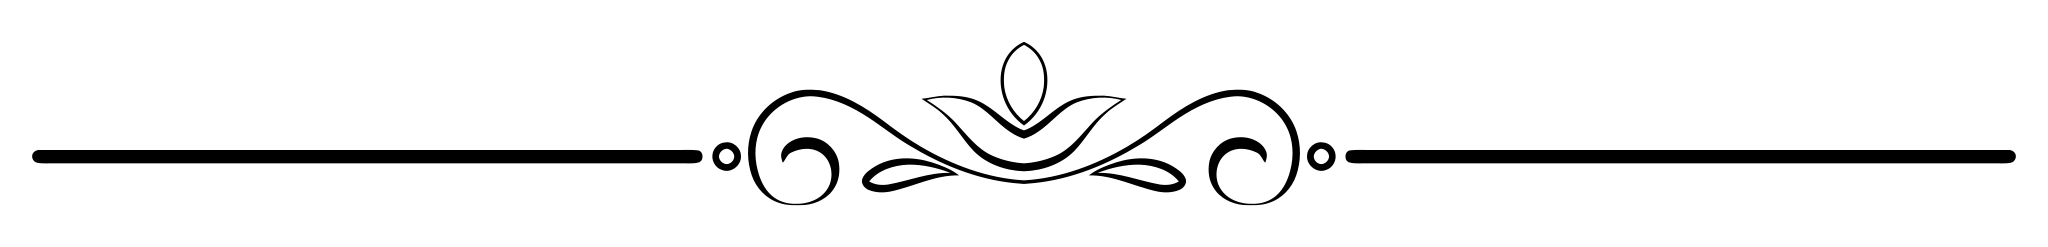
\includegraphics{images/Elegant-Flourish-Frame-Extrapolated-19.svg}

\newpage

Did this puzzle fool you? Welcome to the world of regular expressions!
Both \texttt{pat1} and \texttt{pat2} match the wrong thing, but in
different ways.

If you liked \texttt{pat1}, you've greedily matched too much. The `y'
might occur in later words (per line), and the match won't end until the
last `y' on a line.

\begin{Shaded}
\begin{Highlighting}[]
\OperatorTok{\textgreater{}\textgreater{}\textgreater{}} \ControlFlowTok{for}\NormalTok{ match }\KeywordTok{in}\NormalTok{ re.findall(pat1, txt):}
\NormalTok{...     }\BuiltInTok{print}\NormalTok{(match)}
\NormalTok{...}
\NormalTok{xenarthral xerically xenomorphically}
\NormalTok{xenogenic xenogeny xenophobically}
\NormalTok{xylotomy}
\NormalTok{xenoglossy xanthopterins xenoglossy xeroxed xenophoby}
\NormalTok{xenoglossies xanthoxyls xenoglossias xenomorphically}
\NormalTok{xylopyrography xanthopterines xerochasy}
\end{Highlighting}
\end{Shaded}

On each line, the greedy pattern started at the first `x', which is
often not what you want. Moreover, most lines match multiple words, with
only the line beginning with `xylotomy' happening to be the isolated
word we actually want. The line that begins with `xeroxes' is not
matched at all, which is what we want.

If you liked \texttt{pat2} you often get words, but at other times
either too much \emph{or too little} might be matched. For example, if
`xy' occurs in a longer word, either as a prefix or in the middle, it
can also match.

\begin{Shaded}
\begin{Highlighting}[]
\OperatorTok{\textgreater{}\textgreater{}\textgreater{}} \ControlFlowTok{for}\NormalTok{ match }\KeywordTok{in}\NormalTok{ re.findall(pat2, txt):}
\NormalTok{...     }\BuiltInTok{print}\NormalTok{(match)}
\NormalTok{...}
\NormalTok{...}
\NormalTok{xenarthral xerically}
\NormalTok{xenomorphically}
\NormalTok{xenogenic xenogeny}
\NormalTok{xenophobically}
\NormalTok{xy}
\NormalTok{xenoglossy}
\NormalTok{xanthopterins xenoglossy}
\NormalTok{xeroxed xenophoby}
\NormalTok{xenoglossies xanthoxy}
\NormalTok{xenoglossias xenomorphically}
\NormalTok{xy}
\NormalTok{xanthopterines xerochasy}
\end{Highlighting}
\end{Shaded}

By being non-greedy, we stop when the first `y' is encountered, but as
you see, that still is not quite what we want.

What we actually need to focus on for this task is the \emph{word
boundaries}. Things that are not lowercase letters cannot be part of
matches. In this simple case, non-letters are all spaces and newlines,
but other characters might occur in other texts.

We can be greedy to avoid matching prefixes or infixes, but we also want
to ignore non-letter characters.

\begin{Shaded}
\begin{Highlighting}[]
\OperatorTok{\textgreater{}\textgreater{}\textgreater{}}\NormalTok{ pat3 }\OperatorTok{=}\NormalTok{ re.}\BuiltInTok{compile}\NormalTok{(}\VerbatimStringTok{r\textquotesingle{}x[a{-}z]*y\textquotesingle{}}\NormalTok{)}
\OperatorTok{\textgreater{}\textgreater{}\textgreater{}} \ControlFlowTok{for}\NormalTok{ match }\KeywordTok{in}\NormalTok{ re.findall(pat3, txt):}
\NormalTok{...     }\BuiltInTok{print}\NormalTok{(match)}
\NormalTok{...}
\NormalTok{xerically}
\NormalTok{xenomorphically}
\NormalTok{xenogeny}
\NormalTok{xenophobically}
\NormalTok{xylotomy}
\NormalTok{xenoglossy}
\NormalTok{xenoglossy}
\NormalTok{xenophoby}
\NormalTok{xanthoxy}
\NormalTok{xenomorphically}
\NormalTok{xylopyrography}
\NormalTok{xerochasy}
\end{Highlighting}
\end{Shaded}

Everything we matched, anywhere on each line, had an `x', some other
letters (perhaps including `x's or 'y's along the way), then a 'y'.
Whatever came after each match was a non-letter character.

\newpage

\hypertarget{words-and-sequences}{%
\section{Words and Sequences}\label{words-and-sequences}}

In the previous problem, we identified words that started with `x' and
ended with `y'. You may have noticed, however, that we had already
included the assumption that all the words started with `x'. Perhaps
your solution was clever enough not to fall for the danger shown in this
puzzle. Namely, perhaps not all words will actually start with `x' to
begin with; i.e.~if we try to apply our previous regex to such text.

\begin{Shaded}
\begin{Highlighting}[]
\OperatorTok{\textgreater{}\textgreater{}\textgreater{}}\NormalTok{ txt }\OperatorTok{=} \StringTok{"""}
\StringTok{expurgatory xylometer xenotime xenomorphically exquisitely}
\StringTok{xylology xiphosurans xenophile oxytocin xylogen}
\StringTok{xeriscapes xerochasy inexplicably exabyte inexpressibly}
\StringTok{extremity xiphophyllous xylographic complexly vexillology}
\StringTok{xanthenes xylenol xylol xylenes coextensively}
\StringTok{"""}
\OperatorTok{\textgreater{}\textgreater{}\textgreater{}}\NormalTok{ pat3 }\OperatorTok{=}\NormalTok{ re.}\BuiltInTok{compile}\NormalTok{(}\VerbatimStringTok{r\textquotesingle{}x[a{-}z]*y\textquotesingle{}}\NormalTok{)}
\OperatorTok{\textgreater{}\textgreater{}\textgreater{}}\NormalTok{ re.findall(pat3, txt)}
\NormalTok{[}\StringTok{\textquotesingle{}xpurgatory\textquotesingle{}}\NormalTok{, }\StringTok{\textquotesingle{}xy\textquotesingle{}}\NormalTok{, }\StringTok{\textquotesingle{}xenomorphically\textquotesingle{}}\NormalTok{, }\StringTok{\textquotesingle{}xquisitely\textquotesingle{}}\NormalTok{,}
\StringTok{\textquotesingle{}xylology\textquotesingle{}}\NormalTok{, }\StringTok{\textquotesingle{}xy\textquotesingle{}}\NormalTok{, }\StringTok{\textquotesingle{}xy\textquotesingle{}}\NormalTok{, }\StringTok{\textquotesingle{}xerochasy\textquotesingle{}}\NormalTok{, }\StringTok{\textquotesingle{}xplicably\textquotesingle{}}\NormalTok{, }\StringTok{\textquotesingle{}xaby\textquotesingle{}}\NormalTok{,}
\StringTok{\textquotesingle{}xpressibly\textquotesingle{}}\NormalTok{, }\StringTok{\textquotesingle{}xtremity\textquotesingle{}}\NormalTok{, }\StringTok{\textquotesingle{}xiphophy\textquotesingle{}}\NormalTok{, }\StringTok{\textquotesingle{}xy\textquotesingle{}}\NormalTok{, }\StringTok{\textquotesingle{}xly\textquotesingle{}}\NormalTok{,}
\StringTok{\textquotesingle{}xillology\textquotesingle{}}\NormalTok{, }\StringTok{\textquotesingle{}xy\textquotesingle{}}\NormalTok{, }\StringTok{\textquotesingle{}xy\textquotesingle{}}\NormalTok{, }\StringTok{\textquotesingle{}xy\textquotesingle{}}\NormalTok{, }\StringTok{\textquotesingle{}xtensively\textquotesingle{}}\NormalTok{]}
\end{Highlighting}
\end{Shaded}

As you can see, we matched a number of substrings within words, not only
whole words. What pattern can you use to actually match only words that
start with `x' and end with `y'?

Before you turn the page\ldots{}

\textbf{Think about what defines word boundaries.}

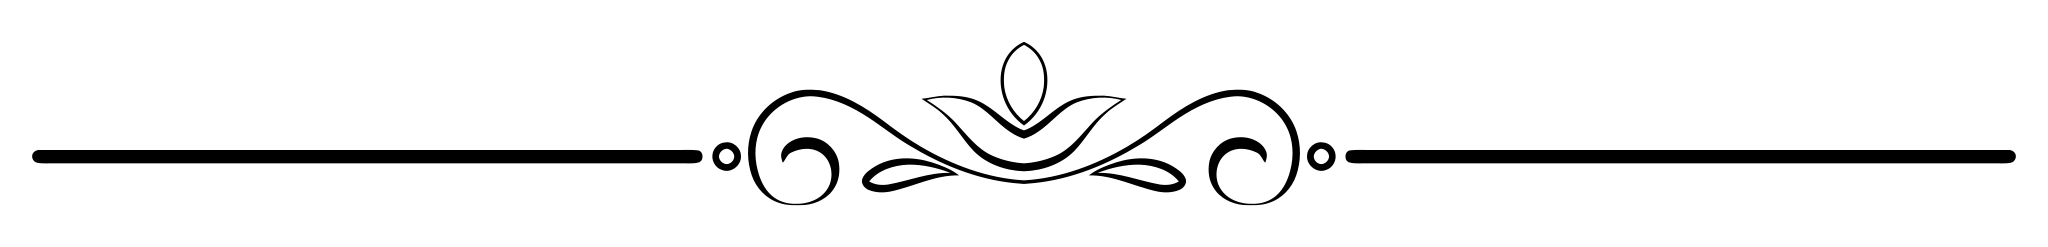
\includegraphics{images/Elegant-Flourish-Frame-Extrapolated-19.svg}

\begin{figure}
\centering
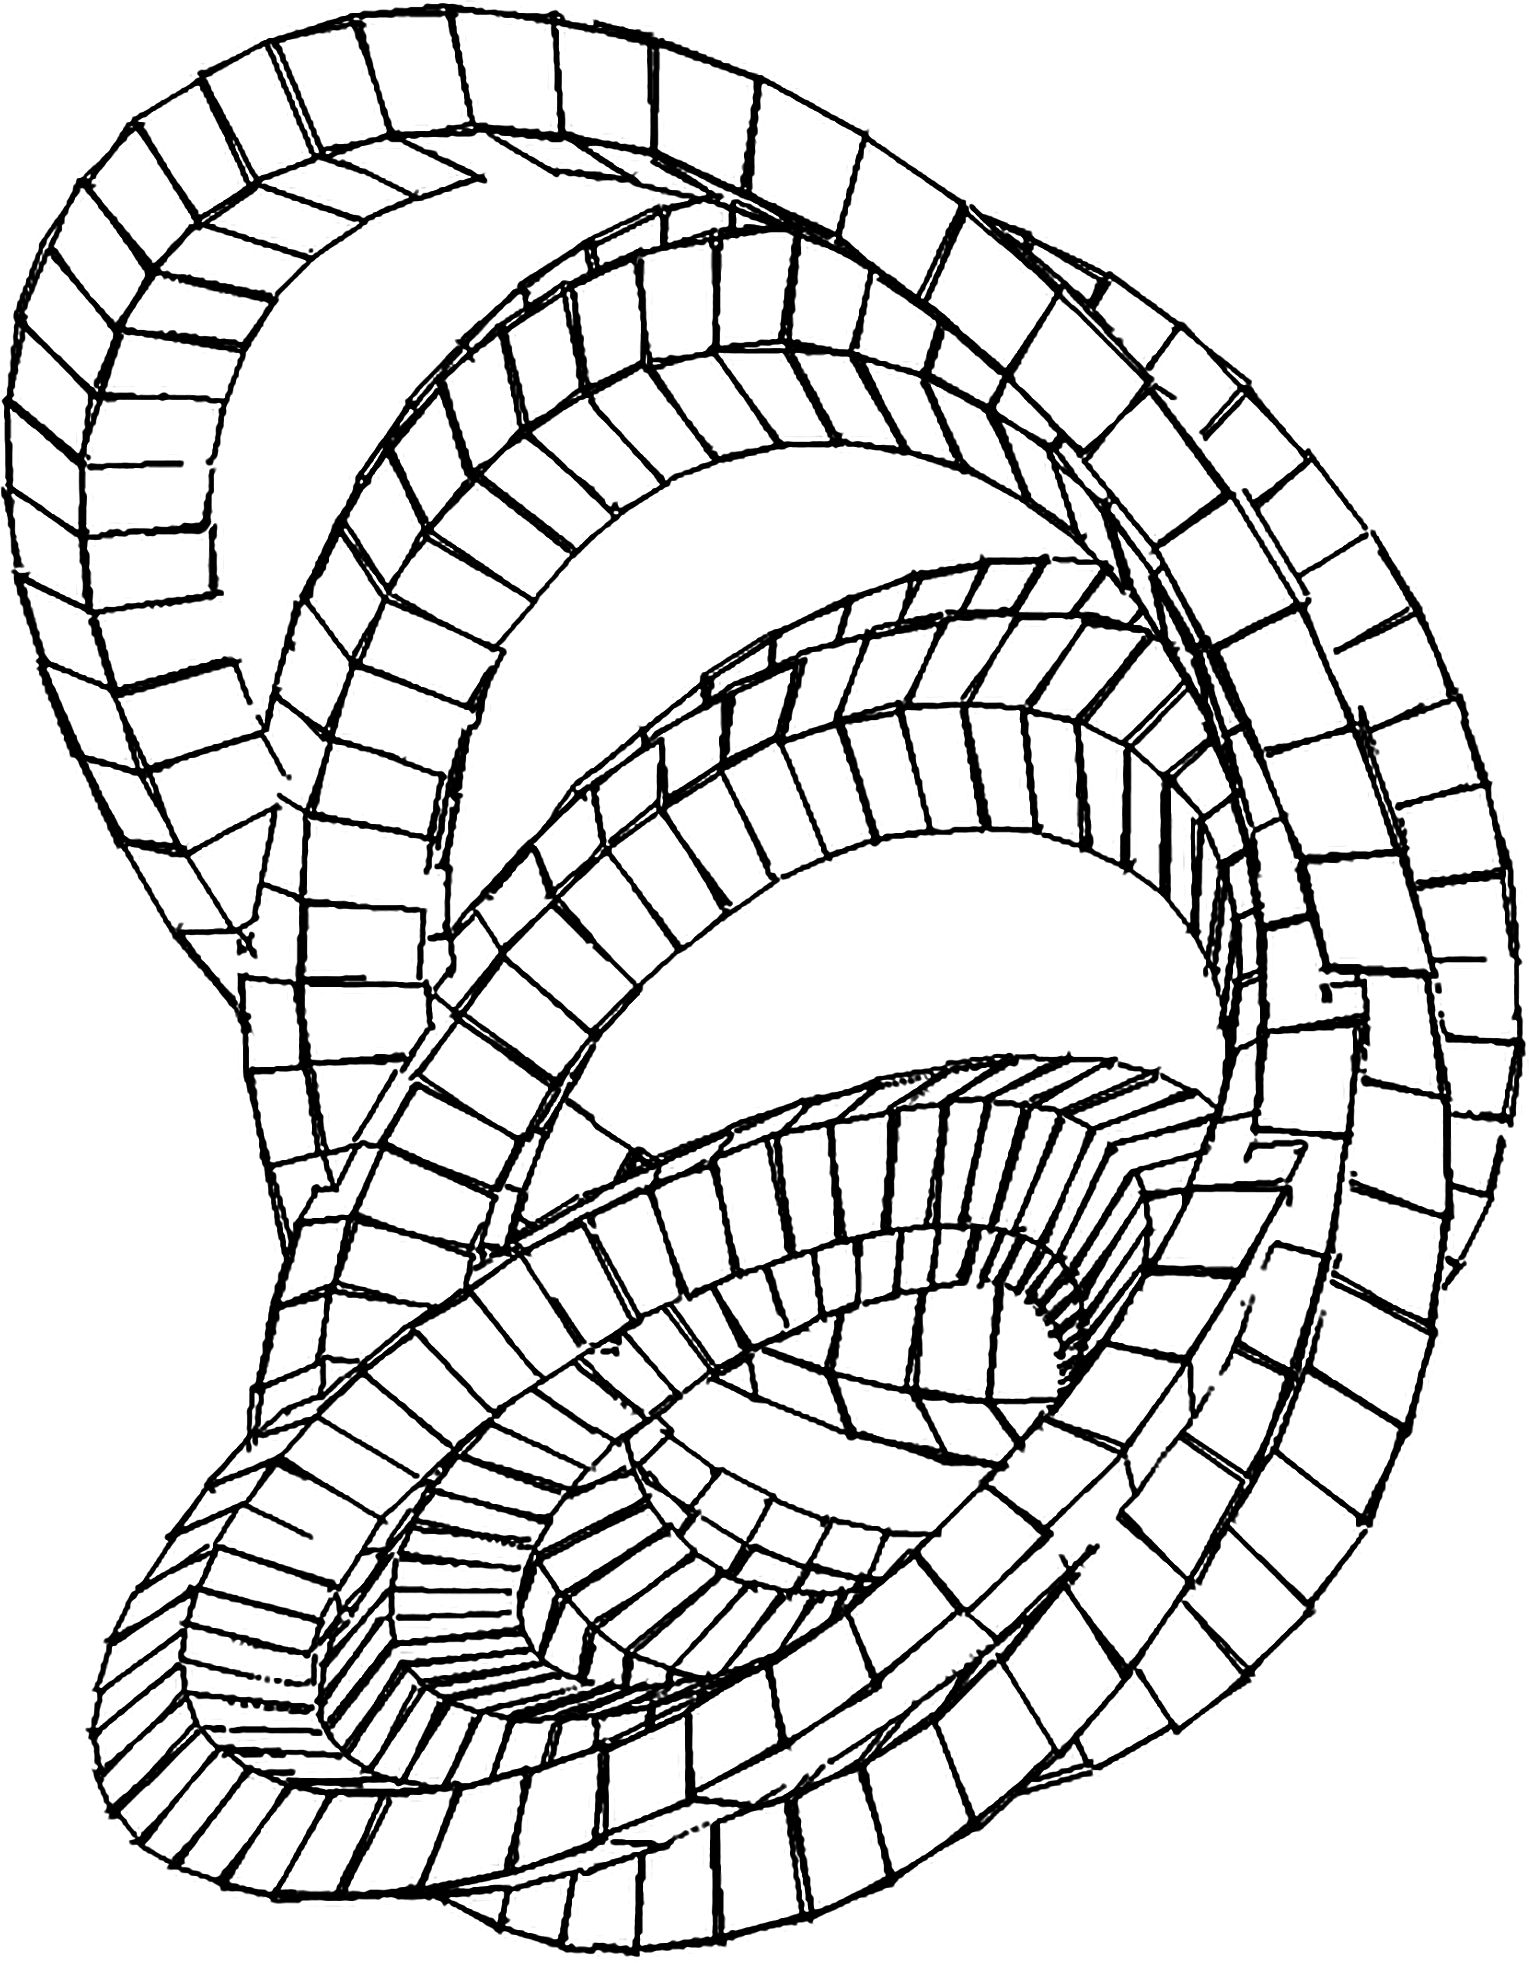
\includegraphics{images/Basket_Recto.png}
\caption{Basket\_Recto}
\end{figure}

\newpage

There are a few ways you might approach this task. The easiest is to use
the explicit ``word boundary'' special \emph{zero-width match} pattern,
spelled as \texttt{\textbackslash{}b} in Python and many other regular
expression engines.

\begin{Shaded}
\begin{Highlighting}[]
\OperatorTok{\textgreater{}\textgreater{}\textgreater{}}\NormalTok{ pat4 }\OperatorTok{=}\NormalTok{ re.}\BuiltInTok{compile}\NormalTok{(}\VerbatimStringTok{r\textquotesingle{}\textbackslash{}bx[a{-}z]*y\textbackslash{}b\textquotesingle{}}\NormalTok{)}
\OperatorTok{\textgreater{}\textgreater{}\textgreater{}}\NormalTok{ re.findall(pat4, txt)}
\NormalTok{[}\StringTok{\textquotesingle{}xenomorphically\textquotesingle{}}\NormalTok{, }\StringTok{\textquotesingle{}xylology\textquotesingle{}}\NormalTok{, }\StringTok{\textquotesingle{}xerochasy\textquotesingle{}}\NormalTok{]}
\end{Highlighting}
\end{Shaded}

Less easy ways to accomplish this include using lookahead and lookbehind
to find non-matching characters that must ``bracket'' the actual match.
For example:

\begin{Shaded}
\begin{Highlighting}[]
\OperatorTok{\textgreater{}\textgreater{}\textgreater{}}\NormalTok{ pat5 }\OperatorTok{=} \VerbatimStringTok{r\textquotesingle{}(?\textless{}=\^{}|(?\textless{}=[\^{}a{-}z]))x[a{-}z]+y(?=$|[\^{}a{-}z])\textquotesingle{}}\NormalTok{)}
\OperatorTok{\textgreater{}\textgreater{}\textgreater{}}\NormalTok{ re.findall(pat5, txt)}
\NormalTok{[}\StringTok{\textquotesingle{}xenomorphically\textquotesingle{}}\NormalTok{, }\StringTok{\textquotesingle{}xylology\textquotesingle{}}\NormalTok{, }\StringTok{\textquotesingle{}xerochasy\textquotesingle{}}\NormalTok{]}
\end{Highlighting}
\end{Shaded}

One trick here is that when we perform a lookbehind assertion, it must
have a fixed width of the match. However, words in our list might either
follow spaces or occur at the start of a line. So we need to create an
alternation between the zero-width lookbehind and the one non-letter
character lookbehind. For the lookahead element, it is enough to say it
is \emph{either} end-of-line (\texttt{\$}) \emph{or} is a non-letter
(\texttt{{[}\^{}a-z{]}}).

\newpage

\hypertarget{endpoint-classes}{%
\section{Endpoint Classes}\label{endpoint-classes}}

This puzzle continues the word matching theme of the last two puzzles.
However, here we have a new wrinkle. We would like to identify
\emph{both} words that start with `x' and end with `y', but \emph{also}
words that start with `y' and end with `x'.

Remembering the word boundary special zero-width pattern we already saw,
a first try at this task might be:

\begin{Shaded}
\begin{Highlighting}[]
\OperatorTok{\textgreater{}\textgreater{}\textgreater{}}\NormalTok{ txt }\OperatorTok{=} \StringTok{"""}
\StringTok{expurgatory xylometer yex xenomorphically exquisitely}
\StringTok{xylology xiphosurans xenophile yunx oxytocin xylogen}
\StringTok{xeriscapes xerochasy inexplicably yonderly inexpressibly}
\StringTok{extremity xerox xylographic complexly vexillology}
\StringTok{xanthenes xylenol xylol yexing xylenes coextensively}

\StringTok{\textgreater{}\textgreater{}\textgreater{} pat6 = re.compile(r\textquotesingle{}}\CharTok{\textbackslash{}b}\StringTok{[xy][a{-}z]*[xy]}\CharTok{\textbackslash{}b}\StringTok{\textquotesingle{})}

\StringTok{\textgreater{}\textgreater{}\textgreater{} re.findall(pat6, txt)}
\StringTok{[\textquotesingle{}yex\textquotesingle{}, \textquotesingle{}xenomorphically\textquotesingle{}, \textquotesingle{}xylology\textquotesingle{}, \textquotesingle{}yunx\textquotesingle{}, \textquotesingle{}xerochasy\textquotesingle{},}
\StringTok{\textquotesingle{}yonderly\textquotesingle{}, \textquotesingle{}xerox\textquotesingle{}]}
\StringTok{"""}
\end{Highlighting}
\end{Shaded}

What went wrong there? Clearly we matched some words we do not want,
even though all of them began with `x' or `y' and ended with `x' or `y'.

Before you turn the page\ldots{}

\textbf{Try to refine the regular expression to match what we want.}

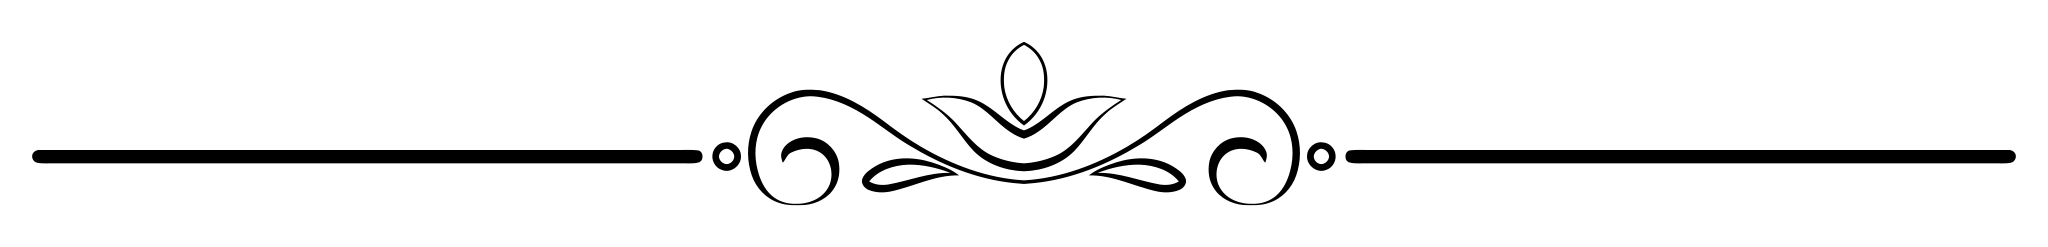
\includegraphics{images/Elegant-Flourish-Frame-Extrapolated-19.svg}

\newpage

The first pattern shown allows for either `x' or `y' to occur at either
the beginning or the end of a word. The word boundaries are handled
fine, but this allows words both beginning and ending with `x', and
likewise beginning and ending with `y'. The character classes at each
end of the overall pattern are independent.

This may seem obvious on reflection, but it is very much like errors I
myself have made embarrassingly many times in real code. A robust
approach is simply to list everything you want as alternatives in a
pattern.

\begin{Shaded}
\begin{Highlighting}[]
\OperatorTok{\textgreater{}\textgreater{}\textgreater{}}\NormalTok{ pat7 }\OperatorTok{=}\NormalTok{ re.}\BuiltInTok{compile}\NormalTok{(}\VerbatimStringTok{r\textquotesingle{}\textbackslash{}b((x[a{-}z]*y)|(y[a{-}z]*x))\textbackslash{}b\textquotesingle{}}\NormalTok{)}
\OperatorTok{\textgreater{}\textgreater{}\textgreater{}}\NormalTok{ [m[}\DecValTok{0}\NormalTok{] }\ControlFlowTok{for}\NormalTok{ m }\KeywordTok{in}\NormalTok{ re.findall(pat7, txt)]}
\NormalTok{[}\StringTok{\textquotesingle{}yex\textquotesingle{}}\NormalTok{, }\StringTok{\textquotesingle{}xenomorphically\textquotesingle{}}\NormalTok{, }\StringTok{\textquotesingle{}xylology\textquotesingle{}}\NormalTok{, }\StringTok{\textquotesingle{}yunx\textquotesingle{}}\NormalTok{, }\StringTok{\textquotesingle{}xerochasy\textquotesingle{}}\NormalTok{]}
\end{Highlighting}
\end{Shaded}

In this solution, there is a little bit of Python-specific detail in the
function API. The function \texttt{re.findall()} returns tuples when a
pattern contains multiple groups. Group 1 will be the whole word, but
one or the other of group 2 and 3 will be blank, i.e.:

\begin{Shaded}
\begin{Highlighting}[]
\OperatorTok{\textgreater{}\textgreater{}\textgreater{}}\NormalTok{ re.findall(pat7, txt)}
\NormalTok{[(}\StringTok{\textquotesingle{}yex\textquotesingle{}}\NormalTok{, }\StringTok{\textquotesingle{}\textquotesingle{}}\NormalTok{, }\StringTok{\textquotesingle{}yex\textquotesingle{}}\NormalTok{),}
\NormalTok{(}\StringTok{\textquotesingle{}xenomorphically\textquotesingle{}}\NormalTok{, }\StringTok{\textquotesingle{}xenomorphically\textquotesingle{}}\NormalTok{, }\StringTok{\textquotesingle{}\textquotesingle{}}\NormalTok{),}
\NormalTok{(}\StringTok{\textquotesingle{}xylology\textquotesingle{}}\NormalTok{, }\StringTok{\textquotesingle{}xylology\textquotesingle{}}\NormalTok{, }\StringTok{\textquotesingle{}\textquotesingle{}}\NormalTok{),}
\NormalTok{(}\StringTok{\textquotesingle{}yunx\textquotesingle{}}\NormalTok{, }\StringTok{\textquotesingle{}\textquotesingle{}}\NormalTok{, }\StringTok{\textquotesingle{}yunx\textquotesingle{}}\NormalTok{),}
\NormalTok{(}\StringTok{\textquotesingle{}xerochasy\textquotesingle{}}\NormalTok{, }\StringTok{\textquotesingle{}xerochasy\textquotesingle{}}\NormalTok{, }\StringTok{\textquotesingle{}\textquotesingle{}}\NormalTok{)]}
\end{Highlighting}
\end{Shaded}

\newpage

\hypertarget{a-configuration-format}{%
\section{A Configuration Format}\label{a-configuration-format}}

This exercise requires just a little bit of Python itself, but is mainly
about choosing the right regular expression. Let's suppose you have a
configuration format that looks like this:

\begin{verbatim}
config = """
3 = foobar
14=baz
9= fizzbuzz
21=more_stuff,here
"""
\end{verbatim}

With a little bit of code, and using a regular expression, you wish to
convert text in this format to a dictionary mapping the numbers to the
left of the equal sign to the strings to the right. For example, the
above example would produce:

\begin{Shaded}
\begin{Highlighting}[]
\NormalTok{\{}\DecValTok{3}\NormalTok{: }\StringTok{\textquotesingle{}foobar\textquotesingle{}}\NormalTok{, }\DecValTok{14}\NormalTok{: }\StringTok{\textquotesingle{}baz\textquotesingle{}}\NormalTok{, }\DecValTok{9}\NormalTok{: }\StringTok{\textquotesingle{}fizzbuzz\textquotesingle{}}\NormalTok{, }\DecValTok{21}\NormalTok{: }\StringTok{\textquotesingle{}more\_stuff,here\textquotesingle{}}\NormalTok{\}}
\end{Highlighting}
\end{Shaded}

Before you turn the page\ldots{}

\textbf{Remember that shapes have edges.}

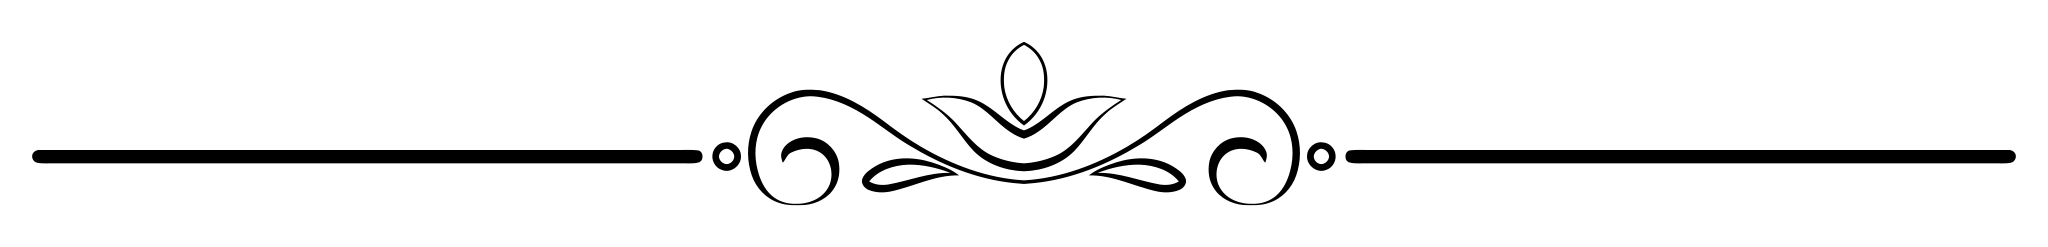
\includegraphics{images/Elegant-Flourish-Frame-Extrapolated-19.svg}

\newpage

As the example shows, there seems to be flexibility in spaces around the
two sides of the equal sign. We should probably assume zero or more
spaces are permitted on either side. The format is probably slightly
surprising in that we would more commonly use words on the left and
numbers on the right in most formats; but it is well-defined enough, and
we can stipulate it has a purpose.

The easiest way to capture the relevant information is probably by using
groups for each side, which will be exposed by \texttt{re.findall()} and
other regular expression functions. We \emph{almost} get the right
answer with this:

\begin{Shaded}
\begin{Highlighting}[]
\OperatorTok{\textgreater{}\textgreater{}\textgreater{}} \BuiltInTok{dict}\NormalTok{(re.findall(}\VerbatimStringTok{r\textquotesingle{}\^{}(\textbackslash{}d+) *= *(.*)$\textquotesingle{}}\NormalTok{, s, re.MULTILINE))}
\NormalTok{\{}\StringTok{\textquotesingle{}3\textquotesingle{}}\NormalTok{: }\StringTok{\textquotesingle{}foobar\textquotesingle{}}\NormalTok{, }\StringTok{\textquotesingle{}14\textquotesingle{}}\NormalTok{: }\StringTok{\textquotesingle{}baz\textquotesingle{}}\NormalTok{, }\StringTok{\textquotesingle{}9\textquotesingle{}}\NormalTok{: }\StringTok{\textquotesingle{}fizzbuzz\textquotesingle{}}\NormalTok{,}
\StringTok{\textquotesingle{}21\textquotesingle{}}\NormalTok{: }\StringTok{\textquotesingle{}more\_stuff,here\textquotesingle{}}\NormalTok{\}}
\end{Highlighting}
\end{Shaded}

Notice that we required the ``multiline'' modifier to match on each line
of the string. The one problem is that the puzzle requested that numbers
appear as numbers, not as strings of digits. There are a number of ways
we might achieve that in Python, but one easy one is:

\begin{Shaded}
\begin{Highlighting}[]
\OperatorTok{\textgreater{}\textgreater{}\textgreater{}}\NormalTok{ \{}\BuiltInTok{int}\NormalTok{(k): v }\ControlFlowTok{for}\NormalTok{ k, v }\KeywordTok{in}
\NormalTok{            re.findall(}\VerbatimStringTok{r\textquotesingle{}\^{}(\textbackslash{}d+) *= *(.*)$\textquotesingle{}}\NormalTok{, s, re.MULTILINE)\}}
\NormalTok{\{}\DecValTok{3}\NormalTok{: }\StringTok{\textquotesingle{}foobar\textquotesingle{}}\NormalTok{, }\DecValTok{14}\NormalTok{: }\StringTok{\textquotesingle{}baz\textquotesingle{}}\NormalTok{, }\DecValTok{9}\NormalTok{: }\StringTok{\textquotesingle{}fizzbuzz\textquotesingle{}}\NormalTok{, }
\DecValTok{21}\NormalTok{: }\StringTok{\textquotesingle{}more\_stuff,here\textquotesingle{}}\NormalTok{\}}
\end{Highlighting}
\end{Shaded}

\begin{figure}
\centering
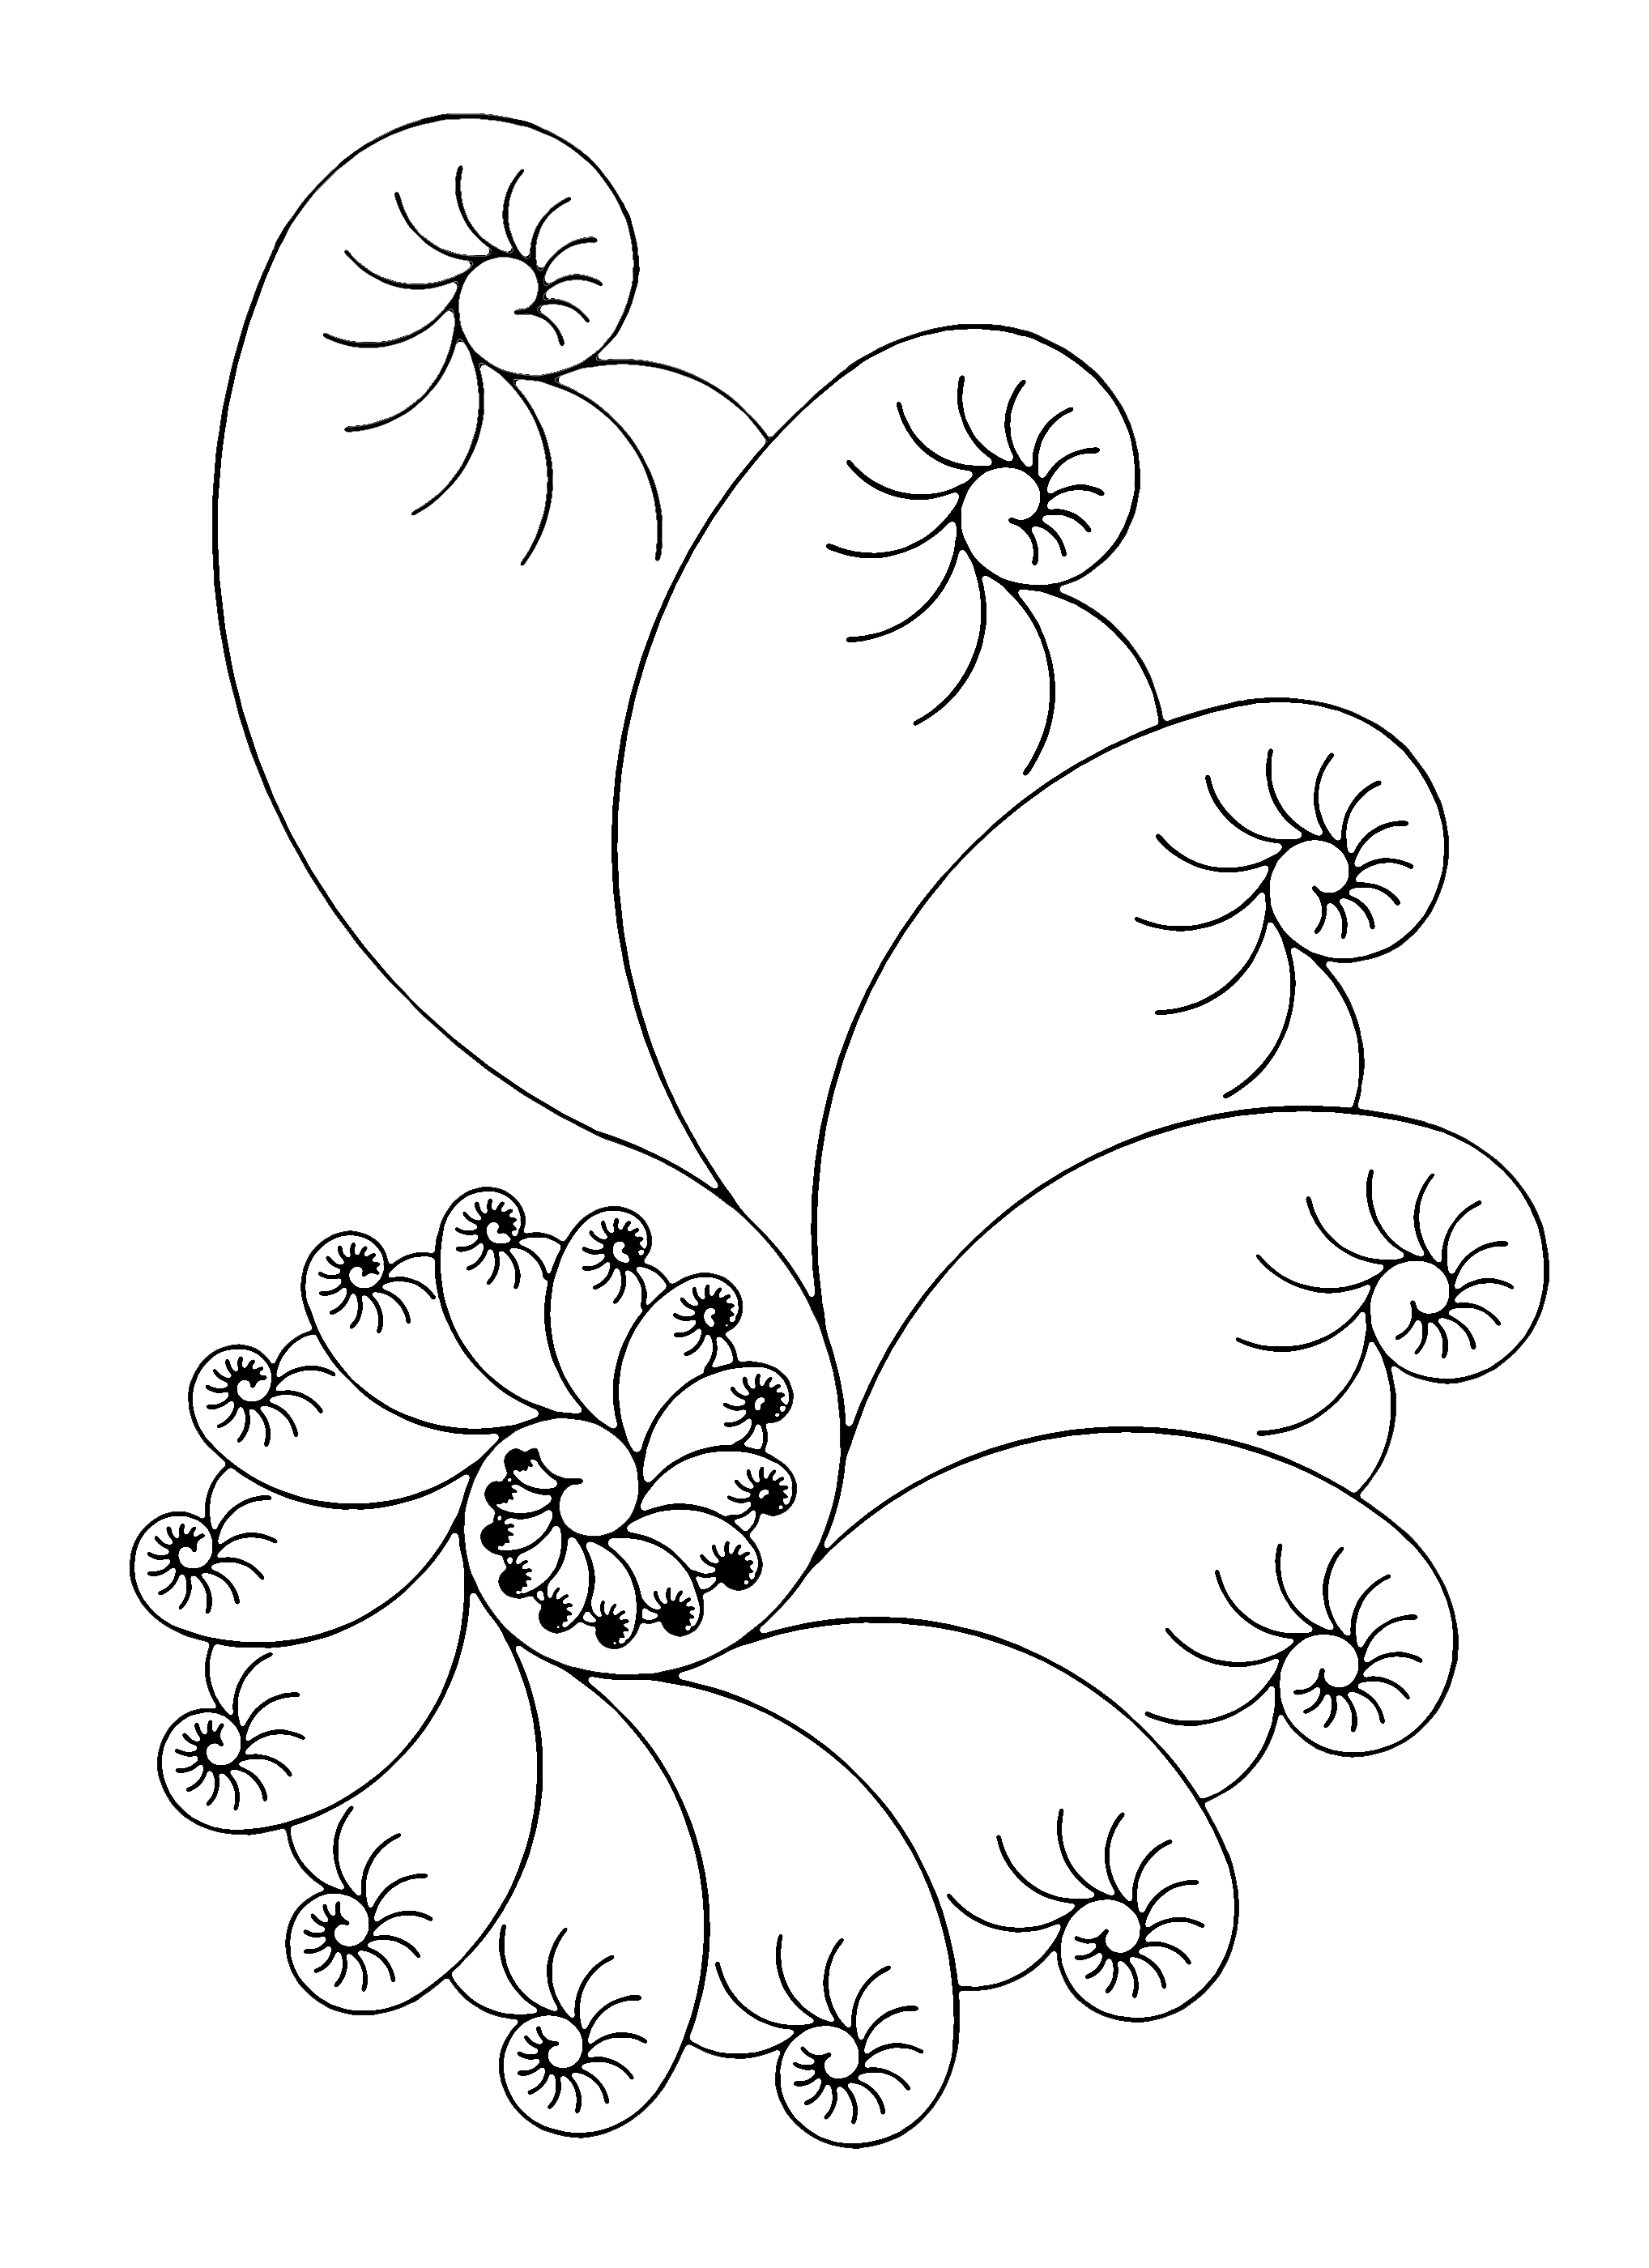
\includegraphics{images/Root5spiral_Recto.png}
\caption{Root5spiral\_Recto}
\end{figure}

\newpage

\hypertarget{the-human-genome}{%
\section{The Human Genome}\label{the-human-genome}}

Genomics commonly uses a format called FASTA to represent genetic
sequences. This puzzle uses a subset of the overall format. Let's
provide just a few quick tips. The letters `A', `C', `G', `T' represent
nucleotide bases in DNA. FASTA may also contain the symbol `N' for
``unknown nucleotide'' and `-' for ``gap of indeterminate length.''

As well, in biological organisms, spans of DNA are terminated by
``telomeres,'' which are special sequences indicating that the read
mechanism should stop transcription and form a protein. Telomeres are
often repeated as much as thousands of times at the ends of sequences.
In a gross simplification for this puzzle, let's suppose that three or
more repetitions of a telomere indicate the end of a sequence for a
protein. In vertebrates, the telomere used is `TTAGGG'.

In this puzzle, we will ignore the marking of the start of a
protein-encoding region, and just assume that all of our strings begin a
potential protein encoding.

You would like to create a regular expression that represents a
``specific protein encoding'' from a (simplified) FASTA fragment. In
particular, we need to know exactly which nucleotides are present, and
gaps or unknown nucleotides will prevent a match. Moreover, even the
telomere repetitions at the end are not permitted (for this puzzle) to
have gaps or unknowns.

For this puzzle, assume that all the FASTA symbols are on a single line.
Normally as published they have a fixed width less than 80 characters;
but newlines are simply ignored. An example of a match:\footnote{Some
  characters shown have Unicode combining diacritics to draw your eye to
  features. Technically, therefore, some characters shown are not
  actually the FASTA codes they look similar to.}

\begin{Shaded}
\begin{Highlighting}[]
\OperatorTok{\textgreater{}\textgreater{}\textgreater{}} \ImportTok{from}\NormalTok{ textwrap }\ImportTok{import}\NormalTok{ wrap}
\OperatorTok{\textgreater{}\textgreater{}\textgreater{}} \BuiltInTok{print}\NormalTok{(}\StringTok{\textquotesingle{}}\CharTok{\textbackslash{}n}\StringTok{\textquotesingle{}}\NormalTok{.join(wrap(valid, }\DecValTok{60}\NormalTok{)))}
\NormalTok{CCCTGAATAATCAAGGTCACAGACCAGTTAGAATGGTTTAGTGTGGAAAGCGGGAAACGA}
\NormalTok{AAAGCCTCTCTGAATCCTGCGCACCGAGATTCTCCCAAGGCAAGGCGAGGGGCTGTATTG}
\NormalTok{CAGGGTTCAACTGCAGCGTCGCAACTCAAATGCAGCATTCCTAATGCACACATGACACCC}
\NormalTok{AAAATATAACAGACATATTACTCATGGAGGGTGAGGGTGAGGGTGAGGGT̠T̠A̠G̠G̠G̠T̠T̠A̠G̠G̠}
\NormalTok{G̠T̠T̠A̠G̠G̠G̠T̠T̠A̠G̠G̠G̠T̠T̠A̠G̠G̠G̠T̠T̠A̠G̠G̠G̠T̠T̠A̠G̠G̠G̠T̠T̠A̠G̠G̠G̠T̠T̠A̠G̠G̠G̠T̠T̠A̠G̠G̠G̠}
\end{Highlighting}
\end{Shaded}

Using a good pattern, we can identify everything up to, but not
including, the telomere repetitions.

\begin{Shaded}
\begin{Highlighting}[]
\OperatorTok{\textgreater{}\textgreater{}\textgreater{}}\NormalTok{ coding }\OperatorTok{=}\NormalTok{ re.search(pat, valid).group()}
\OperatorTok{\textgreater{}\textgreater{}\textgreater{}} \BuiltInTok{print}\NormalTok{(}\StringTok{\textquotesingle{}}\CharTok{\textbackslash{}n}\StringTok{\textquotesingle{}}\NormalTok{.join(wrap(coding, }\DecValTok{60}\NormalTok{)))}
\NormalTok{CCCTGAATAATCAAGGTCACAGACCAGTTAGAATGGTTTAGTGTGGAAAGCGGGAAACGA}
\NormalTok{AAAGCCTCTCTGAATCCTGCGCACCGAGATTCTCCCAAGGCAAGGCGAGGGGCTGTATTG}
\NormalTok{CAGGGTTCAACTGCAGCGTCGCAACTCAAATGCAGCATTCCTAATGCACACATGACACCC}
\NormalTok{AAAACTATAACAGACATATTACTCATGGAGGGTGAGGGTGGGGGTGAGGG}
\end{Highlighting}
\end{Shaded}

The next two are failures. The first does not have sufficient
repetitions. The second has a non-specific nucleotide symbol:

\begin{Shaded}
\begin{Highlighting}[]
\OperatorTok{\textgreater{}\textgreater{}\textgreater{}} \BuiltInTok{print}\NormalTok{(}\StringTok{\textquotesingle{}}\CharTok{\textbackslash{}n}\StringTok{\textquotesingle{}}\NormalTok{.join(wrap(bad\_telomere, }\DecValTok{60}\NormalTok{)))}
\NormalTok{CCCTGAATAATCAAGGTCACAGACCAGTTAGAATGGTTTAGTGTGGAAAGCGGGAAACGA}
\NormalTok{AAAGCCTCTCTGAATCCTGCGCACCGAGATTCTCCCAAGGCAAGGCGAGGGGCTGTATTG}
\NormalTok{CAGGGTTCAACTGCAGCGTCGCAACTCAAATGCAGCATTCCTAATGCACACATGACACCC}
\NormalTok{AAAATATAACAGACATATTACTCATGGAGGGTGAGGGTGAGGGTGAGGGT̠T̠A̠G̠G̠G̠T̠T̠A̠G̠G̠}
\NormalTok{G̠TT̠T̠A̠G̠G̠G̠T̠T̠A̠G̠G̠G̠TT̠T̠A̠G̠G̠G̠GT̠T̠A̠G̠G̠G̠GT̠T̠A̠G̠G̠G̠AT̠T̠A̠G̠G̠G̠T̠T̠A̠G̠G̠G̠TTTAGG}

\OperatorTok{\textgreater{}\textgreater{}\textgreater{}}\NormalTok{ re.search(pat, bad\_telomere) }\KeywordTok{or} \StringTok{"No Match"}
\CommentTok{\textquotesingle{}No Match\textquotesingle{}}

\OperatorTok{\textgreater{}\textgreater{}\textgreater{}} \BuiltInTok{print}\NormalTok{(}\StringTok{\textquotesingle{}}\CharTok{\textbackslash{}n}\StringTok{\textquotesingle{}}\NormalTok{.join(wrap(unknown\_nucleotide, }\DecValTok{60}\NormalTok{)))}
\NormalTok{CCCTGAATAATCAAGGTCACAGACCAGTTAGAATGGTTTAGTGTGGAAAGCGGGAAACGA}
\NormalTok{AAAGCCTCN̅CTGAATCCTGCGCACCGAGATTCTCCCAAGGCAAGGCGAGGGGCTGTATTG}
\NormalTok{CAGGGTTCAACTGCAGCGTCGCAACTCAAATGCAGCATTCCTAATGCACACATGACACCC}
\NormalTok{AAAATATAACAGACATATTACTCATGGAGGGTGAGGGTGAGGGTGAGGGTTAGGGTTAGG}
\NormalTok{GTTTAGGGTTAGGGTTAGGGGTTAGGGGTTAGGGTTAGGGTTAGGGTTAGGG}

\OperatorTok{\textgreater{}\textgreater{}\textgreater{}}\NormalTok{ re.search(pat, unknown\_nucleotide) }\KeywordTok{or} \StringTok{"No Match"}
\CommentTok{\textquotesingle{}No Match\textquotesingle{}}
\end{Highlighting}
\end{Shaded}

In the one mismatch, the first several, but not all trailing bases are
valid telomeres. In the second mismatch, the `N' symbol is used. Both of
these are valid FASTA encoding, but not the sequences specified for
puzzle.

Before you turn the page\ldots{}

\textbf{Remember the central dogma of molecular biology.}

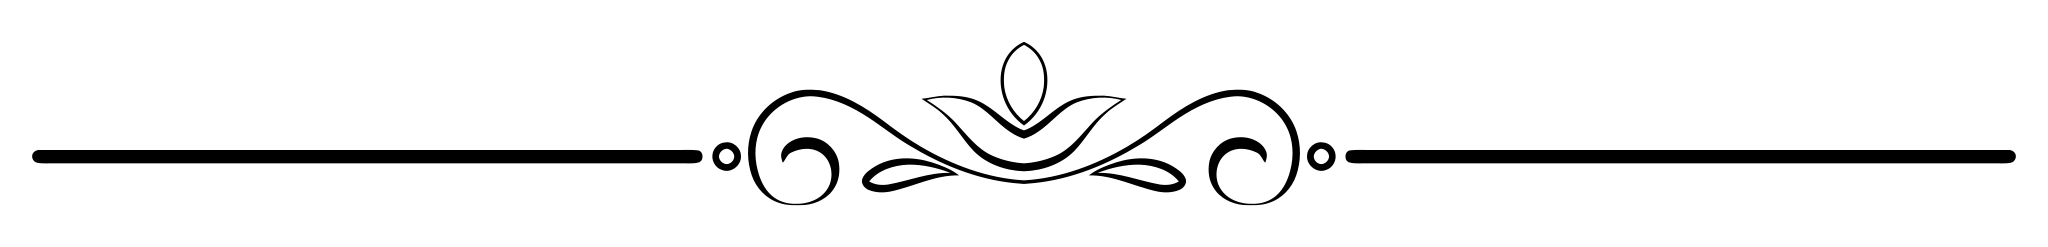
\includegraphics{images/Elegant-Flourish-Frame-Extrapolated-19.svg}

\newpage

There are a few key aspects to keep in mind in designing your regular
expression. You want to make sure that your pattern begins at the start
of the candidate sequence. Otherwise, you could easily match only a
valid tail of it.

From there, any sequence of `C', `A', `T', and `G' symbols is permitted.
However, you definitely want to be non-greedy in matching them since no
telomeres should be included. The telomere may be repeated any number of
times, but at least three. Optionally, repeated telomeres can be
required to continue until the end of the candidate sequence, so we must
match \texttt{\$} \emph{inside} the lookahead pattern.

\begin{Shaded}
\begin{Highlighting}[]
\NormalTok{pat }\OperatorTok{=} \VerbatimStringTok{r\textquotesingle{}\^{}([CATG]+?)(?=(TTAGGG)\{3,\}$)\textquotesingle{}}
\end{Highlighting}
\end{Shaded}

\hypertarget{pitfalls-and-sand-in-the-gears}{%
\chapter{Pitfalls and Sand in the
Gears}\label{pitfalls-and-sand-in-the-gears}}

As compact and expressive as regular expressions can be, there are times
when they simply go disastrously wrong. Be careful to avoid pitfalls,
and at least to understand and identify where such difficulties arise.

\newpage

\hypertarget{catastrophic-backtracking}{%
\section{Catastrophic Backtracking}\label{catastrophic-backtracking}}

In this puzzle, we imagine a certain message protocol (as we do in many
of the other puzzles). We have n message alphabet that consists of the
following symbols:

\begin{longtable}[]{@{}lll@{}}
\toprule
Codepoint & Name & Appearance\tabularnewline
\midrule
\endhead
U+25A0 & Black Square & ■\tabularnewline
U+25AA & Black Small Square & ▪\tabularnewline
U+25CB & White Circle & ○\tabularnewline
U+25C9 & Fisheye & ◉\tabularnewline
U+25A1 & White Square & □\tabularnewline
U+25AB & White Small Square & ▫\tabularnewline
U+25B2 & Black Up Triangle & ▲\tabularnewline
U+25CF & Black Circle & ●\tabularnewline
U+2404 & End Transmition & \texttt{!} (herein)\tabularnewline
\bottomrule
\end{longtable}

These geometric characters are attractive and are chosen to avoid
thinking of matches in terms of natural language words that some other
puzzles utilize. However, feel free in solving it to substitute letters
or numerals, which are probably easier to type in your shell. As long as
the correspondences are one-to-one, it doesn't matter what symbols are
used.

A message in this protocol consists of alternating blocks, belonging to
either ``type 1'' or ``type 2.'' Each block has at least one symbol in
it, but type 1 can have any of black square, black up triangle, white
circle, fisheye, or white square, in any number and order of each. Type
2 blocks, in contrast, may have white small square, white square, black
small square, black circle, or black up triangle, in the same way.
Optionally, a space may separate blocks, but it is not required.

The ``end of transmission'' character indicates the end of a message. An
``obvious'' pattern to describe a valid message apparently matches
appropriately. Some examples are shown below:

\begin{verbatim}
Regex: (^(([■▲○◉□]+) ?([▫□▪●▲]+) ?)+)!

Structure 1/2/1/2  | Message '■▲◉▫■▪▫!' is Valid
Structure 1 2 1 2  | Message '■▲◉ ▫ ■ ▪▫!' is Valid
Missing terminator | Message '■▲◉▫■▪▫' is Invalid
Structure 1 1 2 1  | Message '▲▲▲ ■◉■ ▫▫● ◉○○!' is Invalid
\end{verbatim}

The regex pattern shown actually \emph{is} correct in a mathematical
sense. However, it can also become unworkably slow when checking some
messages. For example:

\begin{verbatim}
Quick match     |
        '■▲○◉□▫□▪●◉◉▫▪▪●●□□▲▲○○◉■◉■▲▲□□◉▲!' is Valid
                |  Checked in 0.00 seconds
Quick failure   |
        '■▲○◉■▲▫▪●●■◉■▲▲◉◉◉■□□□▫▫▪●●●▫■◉■!' is Invalid
                |  Checked in 0.00 seconds
Failure         | '▲□□▲▲□□▲▲▲□□□□□□□□▲▲□▲□▲□▲X' is Invalid
                |  Checked in 4.42 seconds
Slow failure    | '▲□□▲▲▲□□▲▲▲□□□□□□□□▲▲□▲□▲□▲X' is Invalid
                |  Checked in 8.62 seconds
Exponential     | '▲▲▲▲▲▲□□▲▲▲□□□□□□□□▲▲□▲□▲□▲▲X' is Invalid
                |  Checked in 17.59 seconds
One more symbol | '▲▲▲▲□▲□□▲▲□▲□□□□□□□□▲▲□▲□▲□▲▲' is Invalid
                |  Checked in 31.53 seconds
\end{verbatim}

Why does this happen? Both the valid and the first invalid pattern timed
are longer than those that detect mismatches slowly. You can see that
the time to determine the last four messages are invalid approximately
doubles with each additional character.

Before you look at the explanation, both determine why this occurs and
come up with a solution using an alternate regular expression that still
validates the message format. Your solution should take a small fraction
of a second in all cases (even messages that are thousands of symbols
long).

Note that as in other puzzles that use special characters for visual
presentation, you may find experimenting easier if you substitute
letters or numerals that are easy to type for the symbols used here. It
doesn't change the nature of the puzzle at all; it merely might make it
easier to use your keyboard.

Before you turn the page\ldots{}

\textbf{Try hard to avoid catastrophes.}

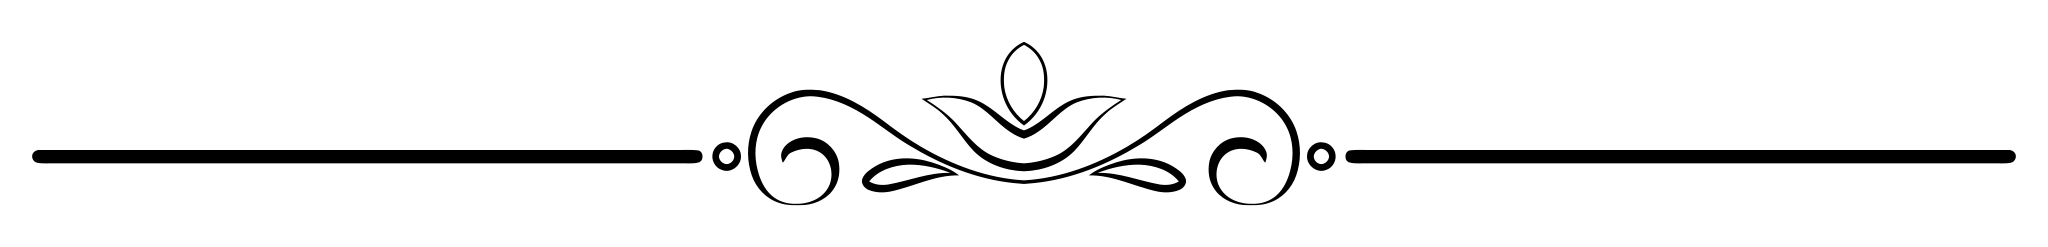
\includegraphics{images/Elegant-Flourish-Frame-Extrapolated-19.svg}

\newpage

The reason why the slow-failing messages fail is somewhat obvious to
human eyes. None of them end with the ``end-of-transmission'' character.
As you can see, whether they end with an entirely invalid symbol
\texttt{X}, or simply with a valid symbol and no terminator, is not
significant.

You may want to think about why the quick-failing message also fails.
Pause for a moment.

But then notice that the final symbol in that message is ``black
square'' which can only occur in type 1 blocks; in the specification, a
type 2 block must always come immediatey before the end-of-transmission
terminator. Nonetheless, the regular expression engine figures that out
in (significantly) less than 1/100th of a second.

What you need to notice is that the symbol set overlaps between type 1
blocks and type 2 blocks. Therefore, it is ambiguous whether a given
symbol belongs to a given block or the next block. If we simply look for
a match, \emph{one possible} match is found quickly, when it exists. For
example, this message that has only the ambiguous ``white square'' and
``black up triangle'' validates immediately:

\begin{verbatim}
Ambiguous quick | '▲▲▲▲□▲□□▲▲□▲□□□□□□□□▲▲□▲□▲□▲▲!' is Valid
                |  Checked in 0.00 seconds
\end{verbatim}

However we do not know how many blocks of type 1 and how many of type 2
were created in the match (pedantically, I know enough about the
internals of the regular expression engine to know that answer, but we
are not guaranteed by the API; it could be different in a later version
of the library without breaking compatibility).

Regular expressions are not smart enough to look ahead to the final
symbol to make sure it is a terminator, unless we tell it to do so. The
produced answer is still \emph{eventually} correct, but it is not as
efficient as we would like.

The engine tries every possible permutation of ``some symbols in this
block, some in that''---which is of exponential complexity on the length
of the message---before it finally decides that none match.

Let's solve that by doing a little extra work for the engine.
Specifically, before we try to identify alternating type 1 and type 2
blocks, let's just make sure that the entire message is made up of valid
symbols that end with the terminator symbol. That check will complete
almost instantly, and will eliminate very many (but not all) ways of
encountering catastrophic backtracking.

\begin{verbatim}
Regex: (^(?=^[■▲○◉□▫▪● ]+!)(([■▲○◉□]+) ?([▫□▪●▲]+) ?)+)!

Structure 1/2/1/2  | Message '■▲◉▫■▪▫!' is Valid
Structure 1 2 1 2  | Message '■▲◉ ▫ ■ ▪▫!' is Valid
Missing terminator | Message '■▲◉▫■▪▫' is Invalid
Structure 1 1 2 1  | Message '▲▲▲ ■■■ ▫▫▫ ○○○!' is Invalid

Quick match     |
        '■▲○◉□▫□▪●◉◉▫▪▪●●□□▲▲○○◉■◉■▲▲□□◉▲!' is Valid
                |  Checked in 0.00 seconds
Quick failure   |
        '■▲○◉■▲▫▪●●■◉■▲▲◉◉◉■□□□▫▫▪●●●▫■◉■!' is Invalid
                |  Checked in 0.00 seconds
Failure         | '▲□□▲▲□□▲▲▲□□□□□□□□▲▲□▲□▲□▲X' is Invalid
                |  Checked in 0.00 seconds
Slow failure    | '▲□□▲▲▲□□▲▲▲□□□□□□□□▲▲□▲□▲□▲X' is Invalid
                |  Checked in 0.00 seconds
Exponential     | '▲▲▲▲▲▲□□▲▲▲□□□□□□□□▲▲□▲□▲□▲▲X' is Invalid
                |  Checked in 0.00 seconds
One more symbol | '▲▲▲▲□▲□□▲▲□▲□□□□□□□□▲▲□▲□▲□▲▲' is Invalid
                |  Checked in 0.00 seconds
Ambiguous quick | '▲▲▲▲□▲□□▲▲□▲□□□□□□□□▲▲□▲□▲□▲▲!' is Valid
                |  Checked in 0.00 seconds
\end{verbatim}

\newpage

\hypertarget{playing-dominoes}{%
\section{Playing Dominoes}\label{playing-dominoes}}

Dominoes is an old family of games dating at least from the Yuan Dynasty
(around 1300 CE). The game is played with tiles on which each half of
one side is marked, generally with a number of dots corresponding to a
number. Specific games vary in their rules, but most require matching
the symbol or number on half of a tile with the corresponding symbol on
another tile.

There are, in fact, Unicode characters for all the domino tiles that
have zero to six dots on each half. We will come back to those
characters in the next puzzle. As a reminder, some of those Unicode
characters are listed in this table.

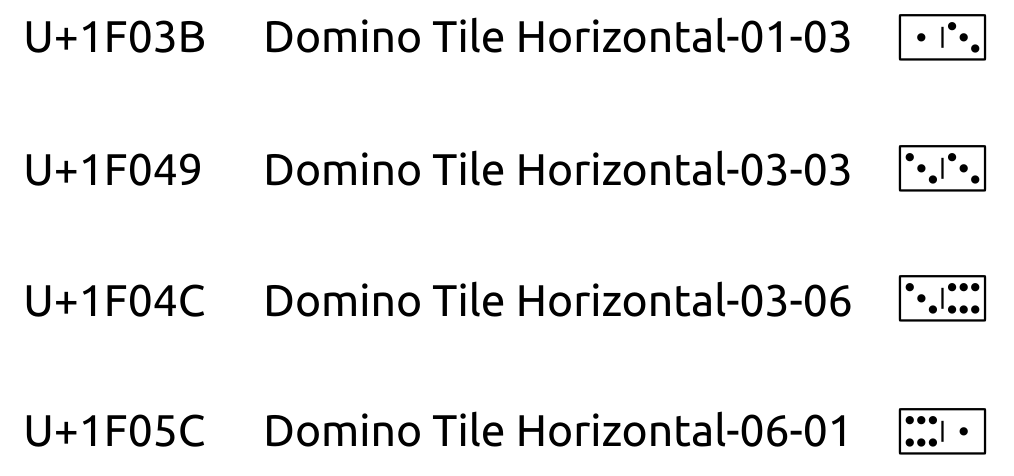
\includegraphics{images/Dominoes-examples.png}

The actual codepoints are hard to enter, and hard to see unless they are
displayed at a large font size (as here). But to illustrate the ``game''
our regex will play, we can show examples of, first, a valid/winning
pattern:

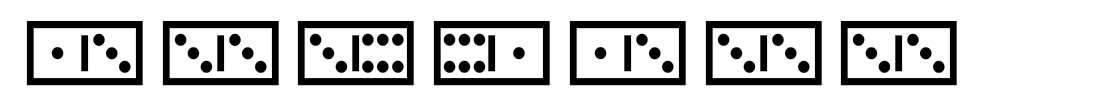
\includegraphics{images/Dominoes-good.png}

And second, an invalid/losing pattern:

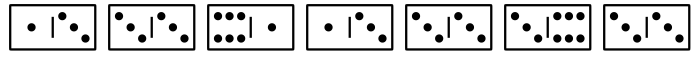
\includegraphics{images/Dominoes-bad.png}

\newpage

In this game, tiles are placed in linear order, and two may occur
adjacently only if they have the same number of dots where they
``touch.'' Unlike with physical tiles, these symbols may not be turned
around, but maintain the same left-right order.

Because of the display and entry problems mentioned, we play an
alternative version of this game in which ``tiles'' are spelled as ASCII
characters. For example, the winning and losing patterns shown as
Unicode characters are as follows in their ASCII versions:

\begin{verbatim}
# Winning
{1:3}{3:3}{3:6}{6:1}{1:3}{3:3}{3:3}

# Losing
{1:3}{3:3}{6:1}{1:3}{3:3}{3:6}{3:3}
\end{verbatim}

Plays may be of any length. Infinitely many tiles, with ends having the
numbers 1-6 in every combination, are available. Write a regular
expression that distinguishes every winning play from a losing play.
Note that any character sequence that doesn't define a series of one or
more tiles is trivially losing.

Before you turn the page\ldots{}

\textbf{You might do this more efficiently than your first thought.}

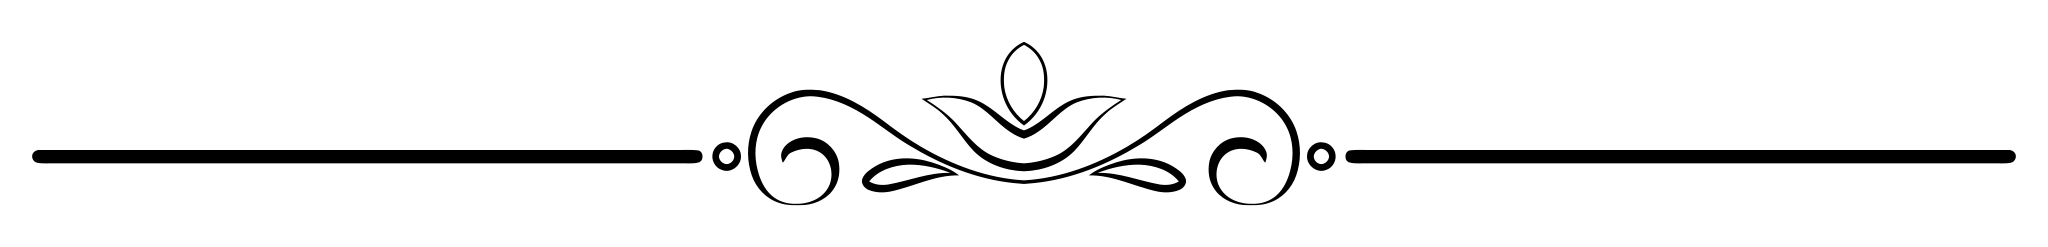
\includegraphics{images/Elegant-Flourish-Frame-Extrapolated-19.svg}

\newpage

Because of our ASCII encoding we have a shortcut available for the
regular expression that can judge whether a play is winning. This would
not be available with the icon characters for the domino tiles.

The same digit must occur at the end of one tile, and again at the start
of the next tile. Therefore, we can shortcut specifically matching '3's
with '3's and '5's with '5's. Instead, we can just use a lookahead to
match a backreference group.

\begin{Shaded}
\begin{Highlighting}[]
\CommentTok{\# Mismatched ends in bad, malformed syntax in awful}
\OperatorTok{\textgreater{}\textgreater{}\textgreater{}}\NormalTok{ good }\OperatorTok{=}  \StringTok{\textquotesingle{}}\SpecialCharTok{\{1:3\}\{3:3\}\{3:6\}\{6:1\}\{1:3\}\{3:3\}\{3:3\}}\StringTok{\textquotesingle{}}
\OperatorTok{\textgreater{}\textgreater{}\textgreater{}}\NormalTok{ bad }\OperatorTok{=}   \StringTok{\textquotesingle{}}\SpecialCharTok{\{1:3\}\{3:3\}\{6:1\}\{1:3\}\{3:3\}\{3:6\}\{3:3\}}\StringTok{\textquotesingle{}} 
\OperatorTok{\textgreater{}\textgreater{}\textgreater{}}\NormalTok{ awful }\OperatorTok{=} \StringTok{\textquotesingle{}}\SpecialCharTok{\{1:3\}\{\{}\StringTok{3:5}\SpecialCharTok{\}\}\{5:2\}}\StringTok{\textquotesingle{}} 

\OperatorTok{\textgreater{}\textgreater{}\textgreater{}}\NormalTok{ pat }\OperatorTok{=} \VerbatimStringTok{r\textquotesingle{}\^{}((\{[1{-}6]:([1{-}6])\})(?=$|\{\textbackslash{}3))+$\textquotesingle{}}

\OperatorTok{\textgreater{}\textgreater{}\textgreater{}} \ControlFlowTok{for}\NormalTok{ play }\KeywordTok{in}\NormalTok{ (good, bad, awful):}
\NormalTok{...     match }\OperatorTok{=}\NormalTok{ re.search(pat, play)}
\NormalTok{...     }\ControlFlowTok{if}\NormalTok{ match:}
\NormalTok{...         }\BuiltInTok{print}\NormalTok{(match.group(), }\StringTok{"wins!"}\NormalTok{)}
\NormalTok{...     }\ControlFlowTok{else}\NormalTok{:}
\NormalTok{...         }\BuiltInTok{print}\NormalTok{(play, }\StringTok{"loses!"}\NormalTok{)}
\NormalTok{...}
\end{Highlighting}
\end{Shaded}

\begin{verbatim}
{1:3}{3:3}{3:6}{6:1}{1:3}{3:3}{3:3} wins!
{1:3}{3:3}{6:1}{1:3}{3:3}{3:6}{3:3} loses!
{1:3}{{3:5}}{5:2} loses!
\end{verbatim}

\begin{figure}
\centering

\includegraphics{images/johnny-automatic-right-hand.svg}
\caption{johnny-automatic-right-hand}
\end{figure}

\newpage

\hypertarget{advanced-dominoes}{%
\section{Advanced Dominoes}\label{advanced-dominoes}}

As the last puzzle showed, there are Unicode characters for domino
tiles. In the last puzzle, we played a game of evaluating whether a
particular sequence of ``tiles''---represented by ASCII sequences---was
winning plays. However, in that last puzzle, we took a shortcut by
taking advantage of the internal structure of the ASCII representation.

It is not too hard to match domino tiles as their Unicode characters.
For example, this pattern matches any linear sequence of (horizontal)
tiles:

\begin{Shaded}
\begin{Highlighting}[]
\NormalTok{pat }\OperatorTok{=}\NormalTok{ (}\VerbatimStringTok{r\textquotesingle{}[\textbackslash{}N\{Domino Tile Horizontal{-}00{-}00\}{-}\textquotesingle{}}
         \StringTok{\textquotesingle{}}\CharTok{\textbackslash{}N\{Domino Tile Horizontal{-}06{-}06\}}\StringTok{]+)\textquotesingle{}}
\end{Highlighting}
\end{Shaded}

Most of those sequences will not be winning plays, of course. Recall the
examples of winning and losing plays from the prior lesson:

Winning:

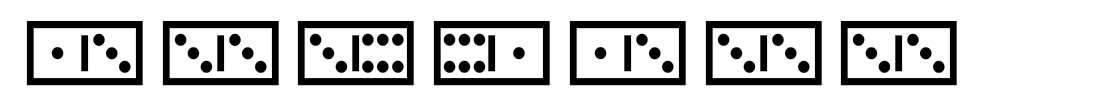
\includegraphics{images/Dominoes-good.png}

Losing:

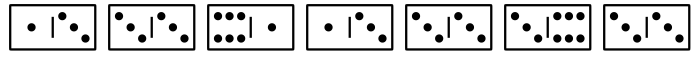
\includegraphics{images/Dominoes-bad.png}

For this game we will simplify in two ways. First, rather than use
hard-to-enter and hard-to-see tile icons, we will use ASCII characters.
In fact, if we only want the tiles with numbers from 1-6 on their ends,
that gives us exactly 36 of them. Conveniently, that happens to be the
same number of symbols as there are numerals plus capital letters (in
English).

However, this puzzle is simplified further by only utilizing four of the
36 possible tiles. Each of those is given the following ASCII
representation. The letters are not mnemonic, but at least they are easy
to type.

\newpage

\begin{longtable}[]{@{}llc@{}}
\toprule
Codepoint & Name & Substitute\tabularnewline
\midrule
\endhead
U+1F03B & Domino Tile Horizontal-01-03 & A\tabularnewline
U+1F049 & Domino Tile Horizontal-03-03 & B\tabularnewline
U+1F04C & Domino Tile Horizontal-03-06 & C\tabularnewline
U+1F05C & Domino Tile Horizontal-06-01 & D\tabularnewline
\bottomrule
\end{longtable}

Repeating our winning and losing examples with this encoding:

\begin{Shaded}
\begin{Highlighting}[]
\NormalTok{win  }\OperatorTok{=} \StringTok{\textquotesingle{}ABCDABB\textquotesingle{}}
\NormalTok{lose }\OperatorTok{=} \StringTok{\textquotesingle{}ABDABCB\textquotesingle{}}
\end{Highlighting}
\end{Shaded}

Plays may be of any length, and you have infinitely many of each of the
four tile types to use. Write a regular expression that distinguishes
every winning play from a losing play. Note that any character outside
the tile symbol set is trivially losing.

Before you turn the page\ldots{}

\textbf{Thoughts about digrams are always pleasant thoughts.}

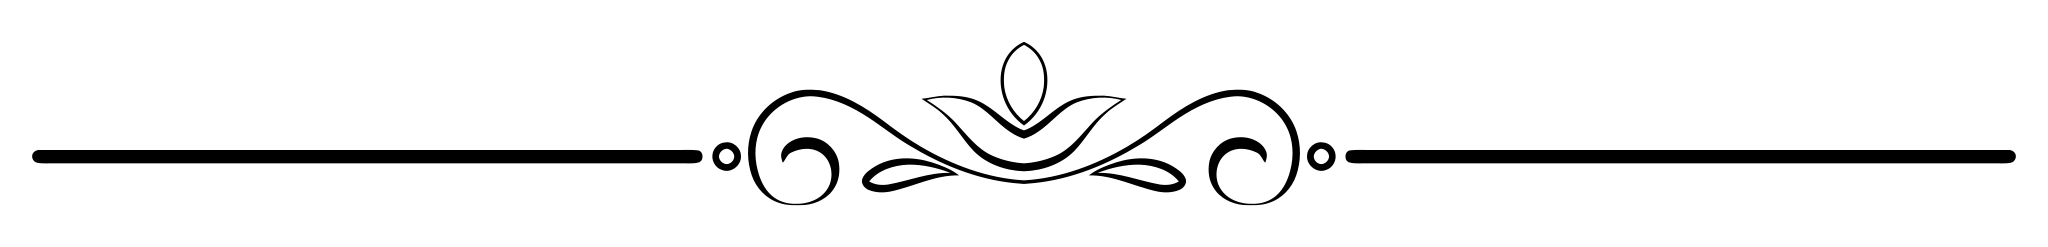
\includegraphics{images/Elegant-Flourish-Frame-Extrapolated-19.svg}

\begin{figure}
\centering
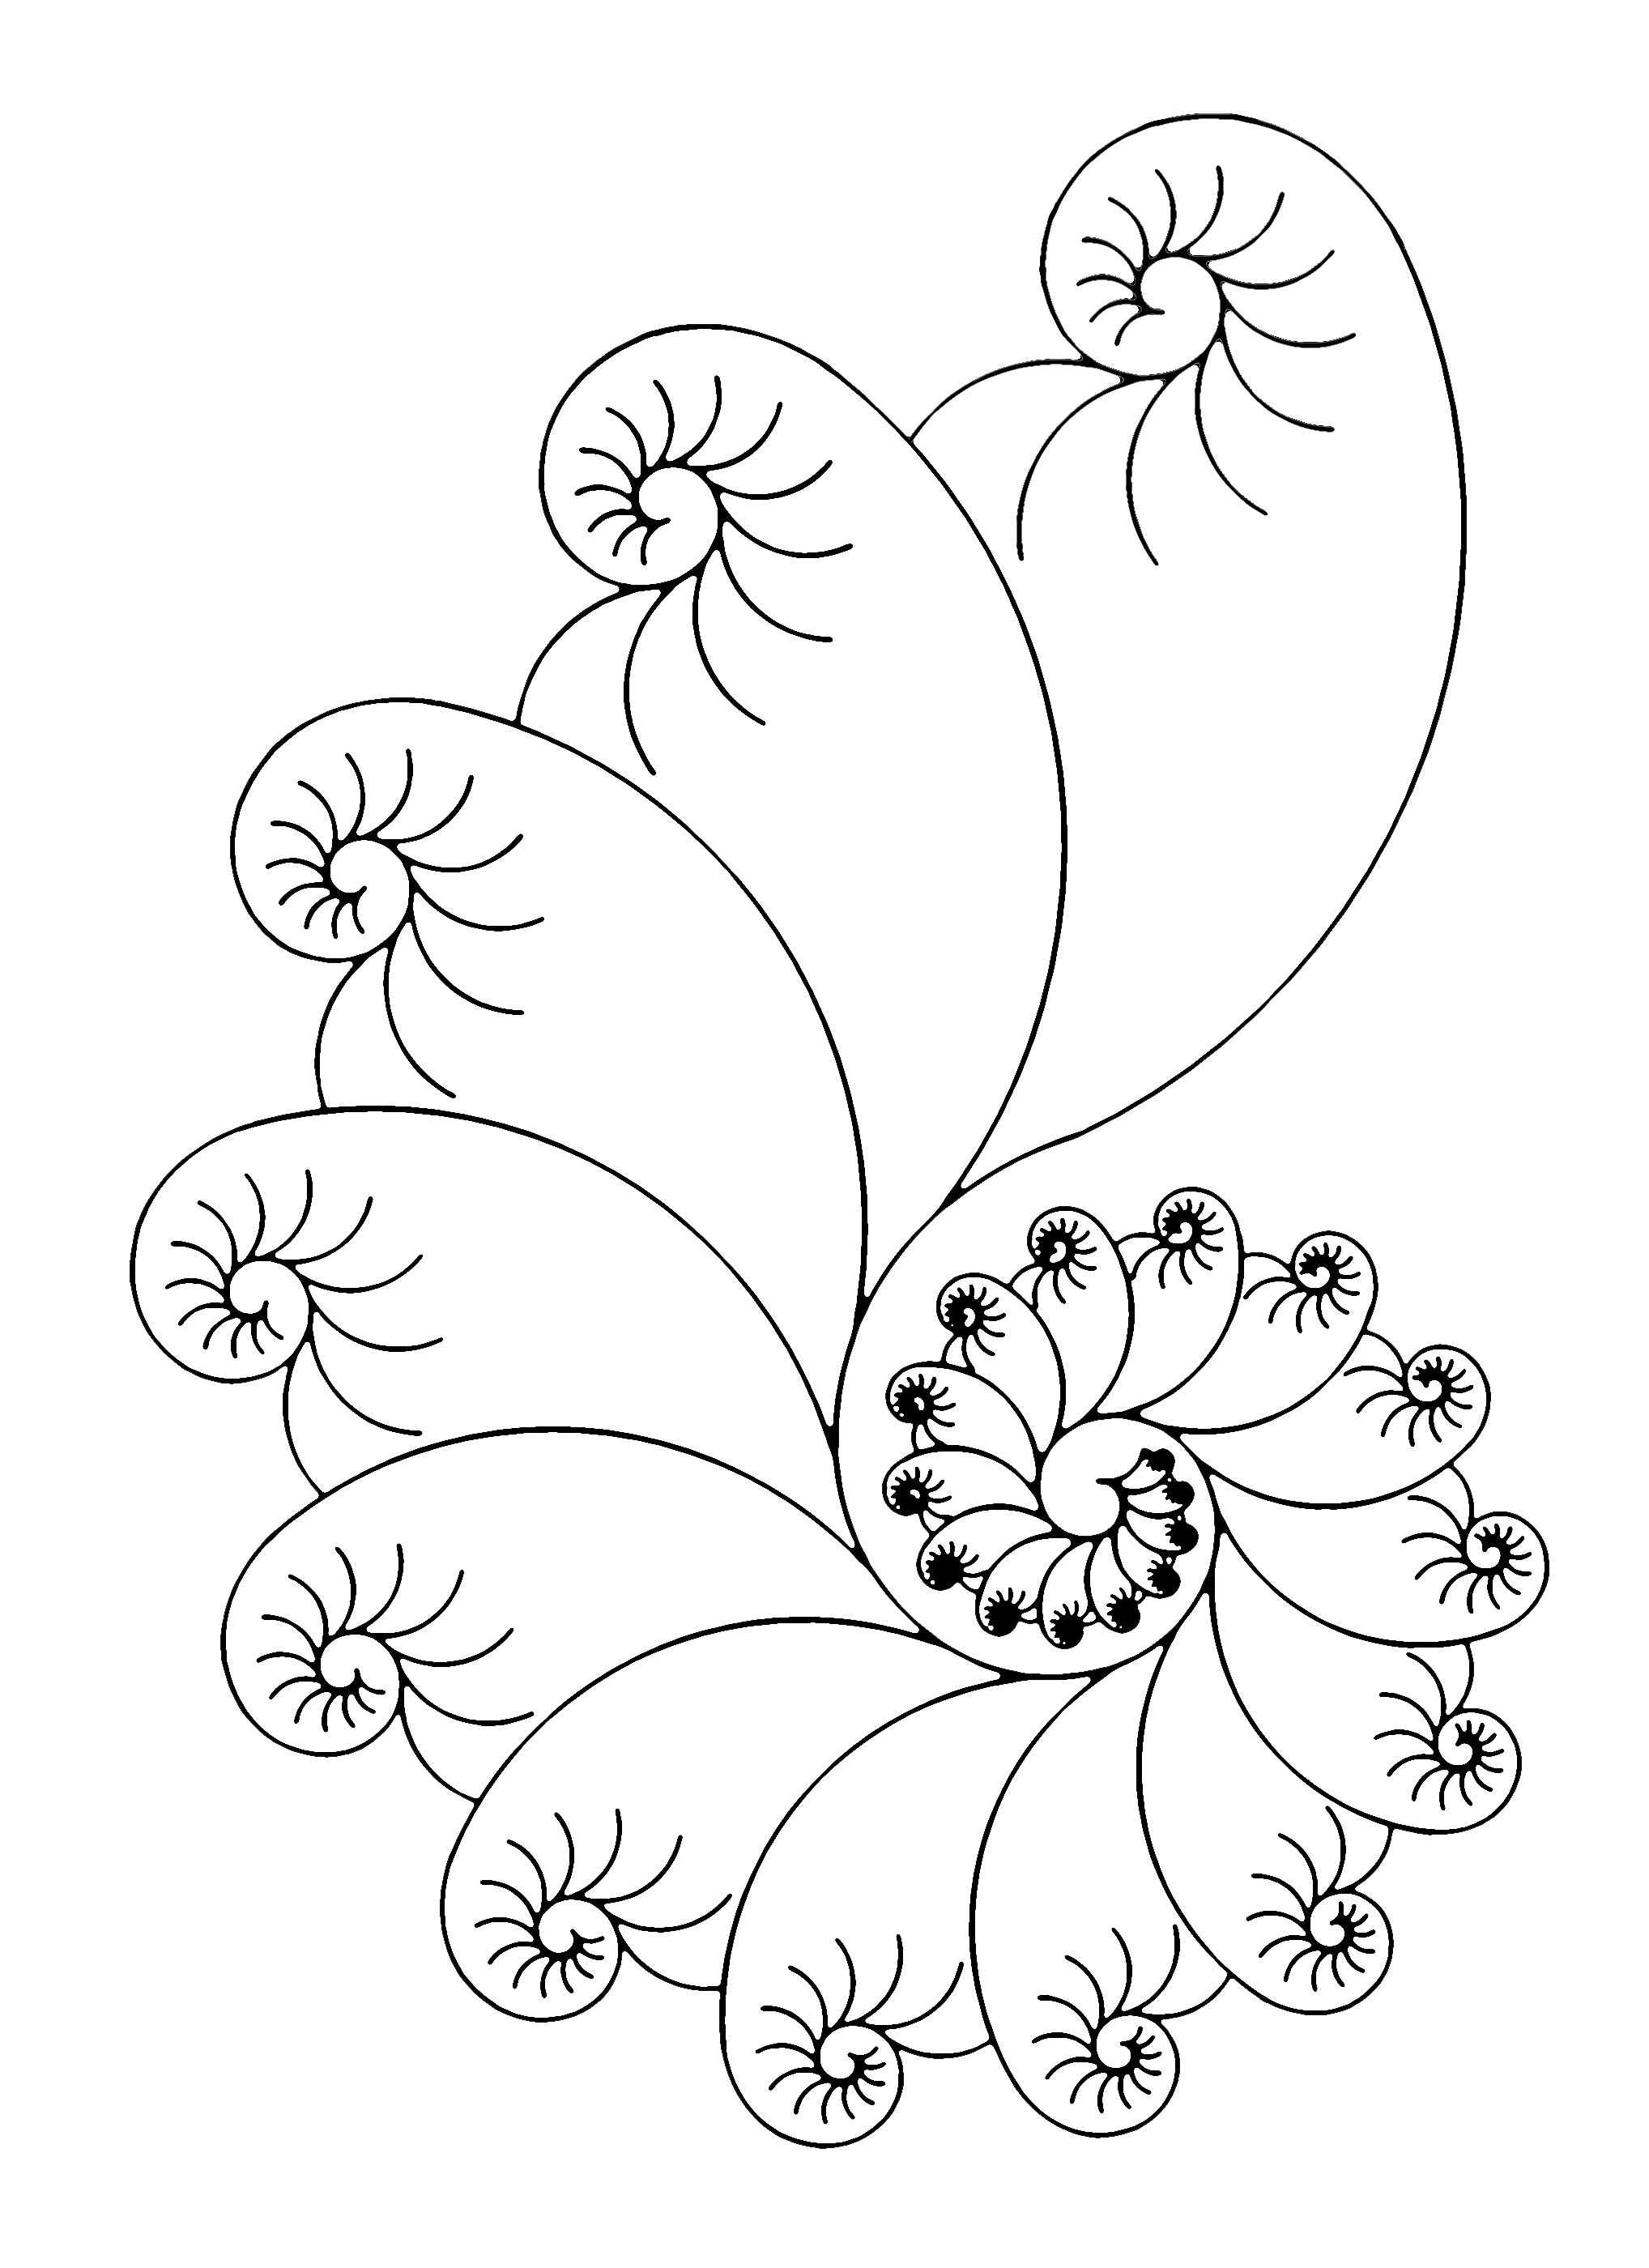
\includegraphics{images/Root5spiral_Verso.png}
\caption{Root5spiral\_Verso}
\end{figure}

\newpage

It probably comes as no surprise to you that a larger tile set would
require a larger regular expression to match winning plays. But the
principle would remain the same if you used more tiles, up to all of
them.

The basic idea here is that you want each tile to be followed by a tile
from some subset of other tiles. Namely, those that begin with the same
number of dots that the current tile ends with.

Of course, a given tile might be the end of a play, so you have to
include that option in your lookahead pattern. You also definitely want
a match to begin at the start of the play and end at the end of the
play, so be sure to include the match patterns \texttt{\^{}} and
\texttt{\$} to indicate that.

\begin{Shaded}
\begin{Highlighting}[]
\OperatorTok{\textgreater{}\textgreater{}\textgreater{}}\NormalTok{ win }\OperatorTok{=} \StringTok{\textquotesingle{}ABCDABB\textquotesingle{}}
\OperatorTok{\textgreater{}\textgreater{}\textgreater{}}\NormalTok{ lose }\OperatorTok{=} \StringTok{\textquotesingle{}ABDABCB\textquotesingle{}}
\OperatorTok{\textgreater{}\textgreater{}\textgreater{}}\NormalTok{ pat }\OperatorTok{=} \VerbatimStringTok{r\textquotesingle{}\^{}(A(?=$|[BC])|B(?=$|[BC])|C(?=$|D)|D(?=$|A))+$\textquotesingle{}}
\OperatorTok{\textgreater{}\textgreater{}\textgreater{}}\NormalTok{ re.search(pat, win)}
\OperatorTok{\textless{}}\NormalTok{re.Match }\BuiltInTok{object}\OperatorTok{;}\NormalTok{ span}\OperatorTok{=}\NormalTok{(}\DecValTok{0}\NormalTok{, }\DecValTok{7}\NormalTok{), match}\OperatorTok{=}\StringTok{\textquotesingle{}ABCDABB\textquotesingle{}}\OperatorTok{\textgreater{}}
\OperatorTok{\textgreater{}\textgreater{}\textgreater{}}\NormalTok{ re.search(pat, lose) }\KeywordTok{or} \StringTok{"No Match"}
\CommentTok{\textquotesingle{}No Match\textquotesingle{}}
\end{Highlighting}
\end{Shaded}

\newpage

\hypertarget{sensor-art}{%
\section{Sensor Art}\label{sensor-art}}

A hypothetical data format uses a character string to represent state
transitions in a two-state system. For example, this might be the status
of some sort of electrical sensor. Each string represents a ``signal''
of some time duration.

The signal can occupy the ``high'' state for any duration, and it can
occupy the ``low'' state for any duration. Moreover, the transition
between the two can either be ``fast'' or ``slow,'' but it must stay in
a state for at least one time interval after each transition.

The format has a mnemonic version that uses simple ASCII art to
represent states and transitions. However, it also has a letter-based
version you may wish to play with instead, simply because many of the
line drawing characters have special meanings in regex syntax. Special
characters can be escaped, but it makes the patterns harder to read.

Some valid and invalid signals are below:

\begin{Shaded}
\begin{Highlighting}[]
\NormalTok{valid\_1a }\OperatorTok{=} \StringTok{"\_/\^{}\^{}\^{}\textbackslash{}\_/\^{}|\_\_\_|\^{}\textbackslash{}\_\_\_\_|\^{}\^{}\textbackslash{}\_\_/"}
\NormalTok{valid\_1b }\OperatorTok{=} \StringTok{"LuHHHdLuHFLLLFHdLLLLFHHdLLu"}
\NormalTok{valid\_2a }\OperatorTok{=} \StringTok{"\_\_\_\_/\^{}\^{}\^{}\^{}\^{}\^{}"}
\NormalTok{valid\_2b }\OperatorTok{=} \StringTok{"LLLLuHHHHHH"}

\NormalTok{invalid\_1a }\OperatorTok{=} \StringTok{"\_\^{}/\^{}\^{}\^{}/\_\_\textbackslash{}\_"}
\NormalTok{invalid\_1b }\OperatorTok{=} \StringTok{"LHuHHHuLLdL"}
\NormalTok{invalid\_2a }\OperatorTok{=} \StringTok{"|\textbackslash{}/|"}
\NormalTok{invalid\_2b }\OperatorTok{=} \StringTok{"FduF"}
\NormalTok{invalid\_3a }\OperatorTok{=} \StringTok{"\_\_/\^{}\^{}|\_\_X\_\_/"}
\NormalTok{invalid\_3b }\OperatorTok{=} \StringTok{"LLuHHFLLXLLu"}
\NormalTok{invalid\_4a }\OperatorTok{=} \StringTok{"|\_\^{}|\_\_"}
\NormalTok{invalid\_4b }\OperatorTok{=} \StringTok{"FLHFLL"}
\end{Highlighting}
\end{Shaded}

Signals \texttt{valid\_1a} and \texttt{valid\_1b} represent the same
measurement. In the correspondence, \texttt{L} maps to \texttt{\_} (low
state), \texttt{u} maps to \texttt{/} (up transition), \texttt{d} maps
to \textbackslash{} (down transition), \texttt{H} maps to \texttt{\^{}}
(high state), and \texttt{F} maps to \texttt{\textbar{}} (fast
transition). Likewise, \texttt{valid\_2a} and \texttt{valid\_2b} are
equivalent and simpler signals with just one up transition, but a
duration in each state.

The invalid signals similarly have the different character options.
Signals \texttt{invalid\_1a} or \texttt{invalid\_1b} have \emph{several}
problems. Low and high states are adjacent with no transition (not
permitted). An alleged up transition occurs from the high state (also
not permitted). Moreover, a down transition occurs from the low state.
The chief problem with \texttt{invalid\_2a} or \texttt{invalid\_2b} are
that they have transitions with no states in between, which is also
prohibited. In the case of \texttt{invalid\_3a} or \texttt{invalid\_3b},
the states and transitions are generally fine, but there is an invalid
symbol thrown in.

You wish to define a regular expression that will match \emph{all} and
\emph{only} valid signal strings. Pick which character set you wish to
define---``ASCII'' or ``linedraw,'' but not intermixed---and find the
pattern you need.

That is, find the pattern that will work \emph{only if} regular
expressions are sufficiently powerful to perform this test.

Before you turn the page\ldots{}

\textbf{Find a matching pattern, if possible.}

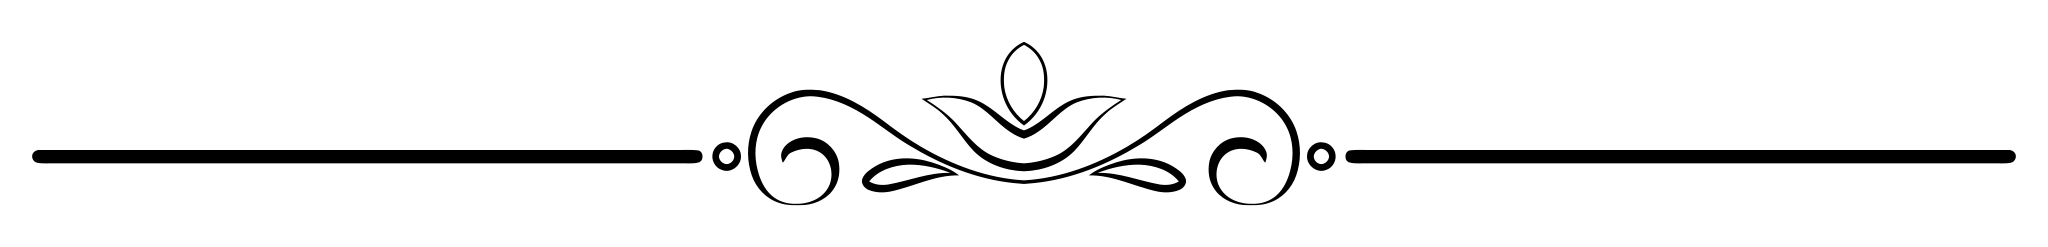
\includegraphics{images/Elegant-Flourish-Frame-Extrapolated-19.svg}

\newpage

This puzzle \emph{is} solvable with regexen. There are a few
observations to keep in mind when thinking about it. The rules for a
valid signal actually consist of just two constraints:

\begin{itemize}
\tightlist
\item
  All signals must be drawn only from the limited alphabet
\item
  Only a subset of \emph{digrams} of symbols are valid
\end{itemize}

In particular, since the alphabet is 5 symbols, there are 25 possible
digrams. However, only 10 of those can occur in a valid signal. You
might be tempted simply to match any number of repetitions of valid
digrams. However, that would go wrong in examples like
\texttt{invalid\_4}. Symbols 1 and 2 might form a valid digram, and
symbols 3 and 4 might also be a valid digram; but quite possibly symbols
2 and 3 are not a valid digram together.

What we need to do is \emph{lookahead} to two symbols, but then only
match one symbol. Moreover, we need to consider the special case where
the regex engine is currently looking at the final symbol in the signal,
since that needs to be included as well. So an alternate lookahead of
``anything then end'' is used. Notice that we can use the `.' wildcard
because the digram was already guaranteed by the \emph{prior} lookahead
in the repetition.

Shown first is \texttt{patB} which matches the ASCII version of the
format, then the much more difficult to read \texttt{patA} which uses
several symbols requiring escaping for the pattern definition since they
would otherwise have regex meanings.

\begin{Shaded}
\begin{Highlighting}[]
\NormalTok{patB }\OperatorTok{=}\NormalTok{  (}\VerbatimStringTok{r\textquotesingle{}\^{}(((?=LL|Lu|LF|HH|Hd|HF|uH|dL|FH|FL)\textquotesingle{}}
         \VerbatimStringTok{r\textquotesingle{}|(?=.$))[LHudF])+$\textquotesingle{}}\NormalTok{)}

\NormalTok{patA }\OperatorTok{=}\NormalTok{  (}\VerbatimStringTok{r\textquotesingle{}\^{}(((?=\_\_|\_/|\_\textbackslash{}||\textbackslash{}\^{}\textbackslash{}\^{}|\textbackslash{}\^{}\textbackslash{}\textbackslash{}|\textbackslash{}\^{}\textbackslash{}||/\textbackslash{}\^{}|\textbackslash{}\textbackslash{}\_|\textbackslash{}|\textbackslash{}\^{}|\textbackslash{}|\_)\textquotesingle{}}
         \VerbatimStringTok{r\textquotesingle{}|(?=.$))[\_\textbackslash{}\^{}/\textbackslash{}\textbackslash{}\textbackslash{}|])+$\textquotesingle{}}\NormalTok{)}
\end{Highlighting}
\end{Shaded}

\hypertarget{creating-functions-using-regexen}{%
\chapter{Creating Functions using
Regexen}\label{creating-functions-using-regexen}}

Very often in Python, or in other programming languages, you will want
to wrap a regular expression in a small function rather than repeat it
inline.

\begin{figure}
\centering

\includegraphics{images/johnny-automatic-left-hand.svg}
\caption{johnny-automatic-left-hand}
\end{figure}

\newpage

\hypertarget{reimplementing-str.count}{%
\section{Reimplementing str.count()}\label{reimplementing-str.count}}

The Python method \texttt{str.count()} is widely useful to find
substrings inside a larger string. For example, here is some typical
code you might write:

\begin{Shaded}
\begin{Highlighting}[]
\CommentTok{\# Lyric from song "Hot Knife" by Fiona Apple}
\OperatorTok{\textgreater{}\textgreater{}\textgreater{}}\NormalTok{ s }\OperatorTok{=} \StringTok{"""If I\textquotesingle{}m butter, if I\textquotesingle{}m butter}
\StringTok{If I\textquotesingle{}m butter, then he\textquotesingle{}s a hot knife}
\StringTok{He makes my heart a CinemaScope screen}
\StringTok{Showing the dancing bird of paradise}
\StringTok{"""}
\OperatorTok{\textgreater{}\textgreater{}\textgreater{}}\NormalTok{ s.count(}\StringTok{\textquotesingle{}e\textquotesingle{}}\NormalTok{)}
\DecValTok{15}
\OperatorTok{\textgreater{}\textgreater{}\textgreater{}}\NormalTok{ s.count(}\StringTok{\textquotesingle{}tt\textquotesingle{}}\NormalTok{)}
\DecValTok{3}
\end{Highlighting}
\end{Shaded}

Imagine that Python did not have the method \texttt{str.count()} but you
wished to implement a similar function by utilizing regular expressions,
with the signature:

\begin{Shaded}
\begin{Highlighting}[]
\KeywordTok{def}\NormalTok{ my\_count(substring: }\BuiltInTok{str}\NormalTok{, string: }\BuiltInTok{str}\NormalTok{) }\OperatorTok{{-}\textgreater{}} \BuiltInTok{int}\NormalTok{:}
    \CommentTok{\# re.sub(..., ...)  \# maybe something like this?}
\NormalTok{    ...}
\end{Highlighting}
\end{Shaded}

Before you turn the page\ldots{}

\textbf{How can a regex count the substring occurrences?}

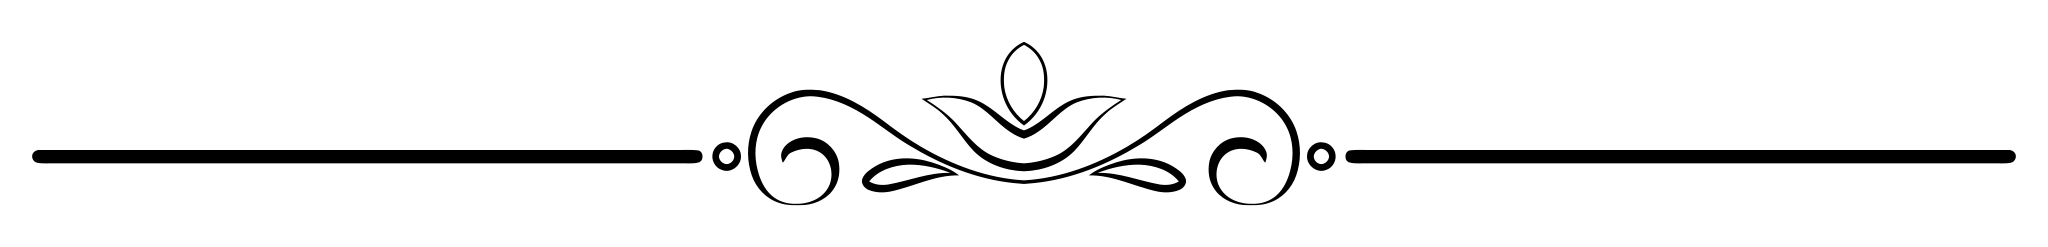
\includegraphics{images/Elegant-Flourish-Frame-Extrapolated-19.svg}

\newpage

Two functions in the Python \texttt{re} module seem especially likely to
be useful. The \texttt{re.sub()} function will replace a pattern with
something else. We might try a solution using that, for example:

\begin{Shaded}
\begin{Highlighting}[]
\OperatorTok{\textgreater{}\textgreater{}\textgreater{}} \KeywordTok{def}\NormalTok{ my\_count(substring, string):}
\NormalTok{...     }\ControlFlowTok{return} \BuiltInTok{len}\NormalTok{(re.sub(}\VerbatimStringTok{fr"[\^{}}\SpecialCharTok{\{}\NormalTok{substring}\SpecialCharTok{\}}\VerbatimStringTok{]"}\NormalTok{, }\StringTok{""}\NormalTok{, string))}
\OperatorTok{\textgreater{}\textgreater{}\textgreater{}}\NormalTok{ my\_count(}\StringTok{\textquotesingle{}e\textquotesingle{}}\NormalTok{, s)}
\DecValTok{15}
\OperatorTok{\textgreater{}\textgreater{}\textgreater{}}\NormalTok{ my\_count(}\StringTok{\textquotesingle{}tt\textquotesingle{}}\NormalTok{, s)   }\CommentTok{\# Oops, this goes wrong}
\DecValTok{10}
\end{Highlighting}
\end{Shaded}

So that try is not quite correct. It will count single characters fine,
but for larger substrings it gets confused. In the example, the
inversion of the character class is \texttt{{[}\^{}tt{]}} which is the
same as simply being \emph{not a ``t''}. In other words, we counted the
``t'''s not the ``tt'''s. Even if the substring hadn't been the same
letter twice, we would count the individual letters in the pattern.

We can fix this with a more complex regular expression (think about how
as a bonus puzzle), but even easier is using \texttt{re.findall()}:

\begin{Shaded}
\begin{Highlighting}[]
\OperatorTok{\textgreater{}\textgreater{}\textgreater{}} \KeywordTok{def}\NormalTok{ my\_count(substring, string):}
\NormalTok{...     }\ControlFlowTok{return} \BuiltInTok{len}\NormalTok{(re.findall(}\VerbatimStringTok{fr"}\SpecialCharTok{\{}\NormalTok{substring}\SpecialCharTok{\}}\VerbatimStringTok{"}\NormalTok{, string))}
\OperatorTok{\textgreater{}\textgreater{}\textgreater{}}\NormalTok{ my\_count(}\StringTok{\textquotesingle{}e\textquotesingle{}}\NormalTok{, s)}
\DecValTok{15}
\OperatorTok{\textgreater{}\textgreater{}\textgreater{}}\NormalTok{ my\_count(}\StringTok{\textquotesingle{}tt\textquotesingle{}}\NormalTok{, s)}
\DecValTok{3}
\end{Highlighting}
\end{Shaded}

\begin{figure}
\centering

\includegraphics{images/Striated_Recto.png}
\caption{Striated\_Recto}
\end{figure}

\newpage

\hypertarget{reimplementing-str.count-stricter}{%
\section{Reimplementing str.count()
(stricter)}\label{reimplementing-str.count-stricter}}

In the last puzzle, we reimplemented \texttt{str.count()} using regular
expressions. However, the solutions I presented---and most likely the
solution you arrvied at on your own---ultimately came down to utilizing
\texttt{len()} on something derived from the original string (to count
the number of matches found).

For this puzzle, pretend that Python also does not have the
\texttt{len()} function; and also do not implement your own equivalent
by, for example, looping through an iterable and incrementing a counter
when a substring is found. One way to express this is that your function
should use no numeric variables or values.

In fact, what we want as the result is a string that represents the
number of the count, not an actual number. To simplify the problem,
however, we can assume that we are only counting single characters, not
substrings in general. In fact, to simplify even more, let's just assume
the input strings are exclusively nucleotide symbols like in the example
below (generalizing this isn't too difficult). A solution will look
something like this:

\begin{Shaded}
\begin{Highlighting}[]
\OperatorTok{\textgreater{}\textgreater{}\textgreater{}} \KeywordTok{def}\NormalTok{ let\_count(char: }\BuiltInTok{str}\NormalTok{, string: }\BuiltInTok{str}\NormalTok{) }\OperatorTok{{-}\textgreater{}} \BuiltInTok{str}\NormalTok{:}
\NormalTok{...     }\CommentTok{\# maybe a while loop, some calls to re.something()}
\NormalTok{        ...}
\end{Highlighting}
\end{Shaded}

For example, using it to count nucleotides:

\begin{Shaded}
\begin{Highlighting}[]
\OperatorTok{\textgreater{}\textgreater{}\textgreater{}}\NormalTok{ mRNA }\OperatorTok{=} \StringTok{\textquotesingle{}\textquotesingle{}\textquotesingle{}}
\StringTok{GGGAAATAAGAGAGAAAAGAAGAGTAAGAAGAAATATAAGACCCCGGCGCCGCCACCAT}
\StringTok{GTTCGTGTTCCTGGTGCTGCTGCCCCTGGTGAGCAGCCAGTGCGTGAACCTGACCACCC}
\StringTok{GGACCCAGCTGCCACCAGCCTACACCAACAGCTTCACCCGGGGCGTCTACTACCCCGAC}
\StringTok{AAGGTGTTCCGGAGCAGCGTCCTGCACAGCACCCAGGACCTGTTCCTGCCCTTCTTCAG}
\StringTok{CAACGTGACCTGGTTCCACGCCATCCACGTGAGCGGCACCAACGGCACCAAGCGGTTCG}
\StringTok{ACAACCCCGTGCTGCCCTTCAACGACGGCGTGTACTTCGCCAGCACCGAGAAGAGCAAC}
\StringTok{ATCATCCGGGGCTGGATCTTCGGCACCACCCTGGACAGCAAGACCCAGAGCCTGCTGAT}
\StringTok{CGTGAATAACGCCACCAACGTGGTGATCAAGGTGTGCGAGTT}
\StringTok{\textquotesingle{}\textquotesingle{}\textquotesingle{}}
\end{Highlighting}
\end{Shaded}

\newpage

\begin{Shaded}
\begin{Highlighting}[]
\OperatorTok{\textgreater{}\textgreater{}\textgreater{}}\NormalTok{ let\_count(}\StringTok{\textquotesingle{}G\textquotesingle{}}\NormalTok{, mRNA)}
\CommentTok{\textquotesingle{}120\textquotesingle{}}
\OperatorTok{\textgreater{}\textgreater{}\textgreater{}}\NormalTok{ let\_count(}\StringTok{\textquotesingle{}C\textquotesingle{}}\NormalTok{, mRNA)}
\CommentTok{\textquotesingle{}152\textquotesingle{}}
\OperatorTok{\textgreater{}\textgreater{}\textgreater{}}\NormalTok{ let\_count(}\StringTok{\textquotesingle{}T\textquotesingle{}}\NormalTok{, mRNA)}
\CommentTok{\textquotesingle{}74\textquotesingle{}}
\OperatorTok{\textgreater{}\textgreater{}\textgreater{}}\NormalTok{ let\_count(}\StringTok{\textquotesingle{}A\textquotesingle{}}\NormalTok{, mRNA)}
\CommentTok{\textquotesingle{}109\textquotesingle{}}
\end{Highlighting}
\end{Shaded}

Before you turn the page\ldots{}

\textbf{Write a Python function with the restrictions given.}

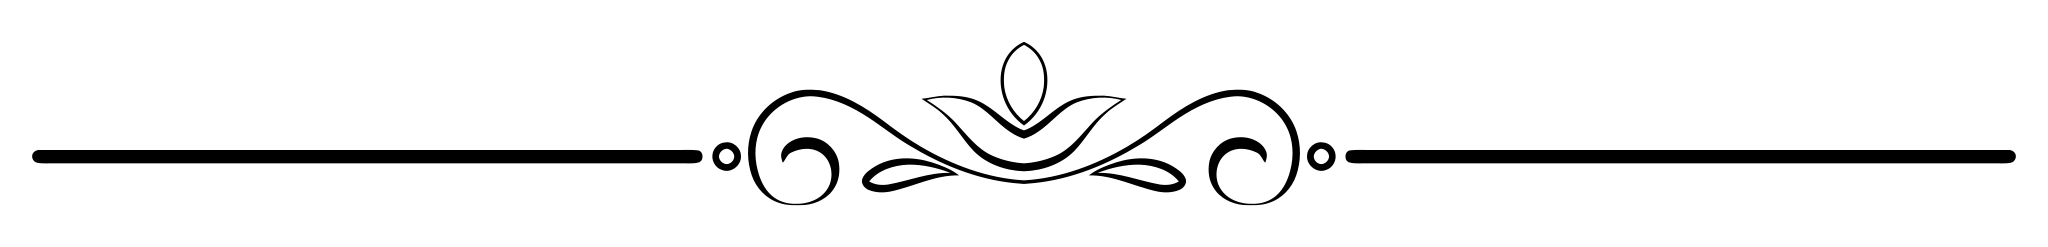
\includegraphics{images/Elegant-Flourish-Frame-Extrapolated-19.svg}

\newpage

This one turns out to be somewhat difficult, but also to be
\emph{possible}, which is itself sort of amazing. No numbers whatsoever
are involved in the solution shown. No counters, no integer variables,
no Python functions returning numbers.

We also do not need to use any Python string methods, although it is
fair to note that some of what is performed via regular expressions
might be more simple to express as string methods. The function can
perform strictly and only regular expression operations\ldots{} along
with a little bit of Python looping (but never over numbers).

We use two sentinels in alternation for the loop, indicating either the
number of items at a certain power of ten, or the number at the next
higher power. A dictionary can map zero to nine repetitions of a
sentinel to the corresponding numeral, but leave the rest of the string
unchanged.

\begin{Shaded}
\begin{Highlighting}[]
\CommentTok{\# Group 1: zero or more leading @\textquotesingle{}s}
\CommentTok{\# Group 2: some specific number of \_\textquotesingle{}s}
\CommentTok{\# Group 3: anything until end; digits expected}
\NormalTok{counter }\OperatorTok{=}\NormalTok{ \{}
    \VerbatimStringTok{r\textquotesingle{}(\^{}@*)(\_\_\_\_\_\_\_\_\_)(.*$)\textquotesingle{}}\NormalTok{: }\VerbatimStringTok{r\textquotesingle{}\textbackslash{}g\textless{}1\textgreater{}9\textbackslash{}g\textless{}3\textgreater{}\textquotesingle{}}\NormalTok{,}
    \VerbatimStringTok{r\textquotesingle{}(\^{}@*)(\_\_\_\_\_\_\_\_)(.*$)\textquotesingle{}}\NormalTok{: }\VerbatimStringTok{r\textquotesingle{}\textbackslash{}g\textless{}1\textgreater{}8\textbackslash{}g\textless{}3\textgreater{}\textquotesingle{}}\NormalTok{,}
    \VerbatimStringTok{r\textquotesingle{}(\^{}@*)(\_\_\_\_\_\_\_)(.*$)\textquotesingle{}}\NormalTok{: }\VerbatimStringTok{r\textquotesingle{}\textbackslash{}g\textless{}1\textgreater{}7\textbackslash{}g\textless{}3\textgreater{}\textquotesingle{}}\NormalTok{,}
    \VerbatimStringTok{r\textquotesingle{}(\^{}@*)(\_\_\_\_\_\_)(.*$)\textquotesingle{}}\NormalTok{: }\VerbatimStringTok{r\textquotesingle{}\textbackslash{}g\textless{}1\textgreater{}6\textbackslash{}g\textless{}3\textgreater{}\textquotesingle{}}\NormalTok{,}
    \VerbatimStringTok{r\textquotesingle{}(\^{}@*)(\_\_\_\_\_)(.*$)\textquotesingle{}}\NormalTok{: }\VerbatimStringTok{r\textquotesingle{}\textbackslash{}g\textless{}1\textgreater{}5\textbackslash{}g\textless{}3\textgreater{}\textquotesingle{}}\NormalTok{,}
    \VerbatimStringTok{r\textquotesingle{}(\^{}@*)(\_\_\_\_)(.*$)\textquotesingle{}}\NormalTok{: }\VerbatimStringTok{r\textquotesingle{}\textbackslash{}g\textless{}1\textgreater{}4\textbackslash{}g\textless{}3\textgreater{}\textquotesingle{}}\NormalTok{,}
    \VerbatimStringTok{r\textquotesingle{}(\^{}@*)(\_\_\_)(.*$)\textquotesingle{}}\NormalTok{: }\VerbatimStringTok{r\textquotesingle{}\textbackslash{}g\textless{}1\textgreater{}3\textbackslash{}g\textless{}3\textgreater{}\textquotesingle{}}\NormalTok{,}
    \VerbatimStringTok{r\textquotesingle{}(\^{}@*)(\_\_)(.*$)\textquotesingle{}}\NormalTok{: }\VerbatimStringTok{r\textquotesingle{}\textbackslash{}g\textless{}1\textgreater{}2\textbackslash{}g\textless{}3\textgreater{}\textquotesingle{}}\NormalTok{,}
    \VerbatimStringTok{r\textquotesingle{}(\^{}@*)(\_)(.*$)\textquotesingle{}}\NormalTok{: }\VerbatimStringTok{r\textquotesingle{}\textbackslash{}g\textless{}1\textgreater{}1\textbackslash{}g\textless{}3\textgreater{}\textquotesingle{}}\NormalTok{,}
    \VerbatimStringTok{r\textquotesingle{}(\^{}@*)(\_*)(.*$)\textquotesingle{}}\NormalTok{: }\VerbatimStringTok{r\textquotesingle{}\textbackslash{}g\textless{}1\textgreater{}0\textbackslash{}g\textless{}3\textgreater{}\textquotesingle{}}
\NormalTok{\}}
\end{Highlighting}
\end{Shaded}

A first step is to map the target character to a sentinel. It would be
easy to extend the main function to map a generic regular expression
pattern to that same sentinel.

The two sentinels underscore and at-sign are used here, but some rare
Unicode codepoint in the astral plane---or even a private-use
codepoint---could just as well be used instead if collision with the
initial string were a concern.

\newpage

\begin{Shaded}
\begin{Highlighting}[]
\KeywordTok{def}\NormalTok{ let\_count(c, s):}
    \CommentTok{\# First lines only convert single char to sentinel,}
    \CommentTok{\# but could be generalized to any regex pattern}
    \CommentTok{\# Remove everything that isn\textquotesingle{}t the target character}
\NormalTok{    s }\OperatorTok{=}\NormalTok{ re.sub(}\VerbatimStringTok{fr\textquotesingle{}[\^{}}\SpecialCharTok{\{c\}}\VerbatimStringTok{]\textquotesingle{}}\NormalTok{, }\StringTok{\textquotesingle{}\textquotesingle{}}\NormalTok{, s)}
    \CommentTok{\# Convert the target to the underscore sentinel}
\NormalTok{    s }\OperatorTok{=}\NormalTok{ re.sub(}\VerbatimStringTok{fr\textquotesingle{}}\SpecialCharTok{\{c\}}\VerbatimStringTok{\textquotesingle{}}\NormalTok{, }\StringTok{\textquotesingle{}\_\textquotesingle{}}\NormalTok{, s)}

    \CommentTok{\# Loop indefinitely: do not know number digits needed}
    \ControlFlowTok{while} \VariableTok{True}\NormalTok{:}
        \CommentTok{\# Ten underscores become an @ sign}
\NormalTok{        s }\OperatorTok{=}\NormalTok{ re.sub(}\VerbatimStringTok{r\textquotesingle{}\_\_\_\_\_\_\_\_\_\_\textquotesingle{}}\NormalTok{, }\StringTok{\textquotesingle{}@\textquotesingle{}}\NormalTok{, s)}
        \ControlFlowTok{for}\NormalTok{ k, v }\KeywordTok{in}\NormalTok{ counter.items():}
            \CommentTok{\# Replace trailing underscores with a digit}
\NormalTok{            new }\OperatorTok{=}\NormalTok{ re.sub(k, v, s)}
            \CommentTok{\# Some pattern matched, so exit the loop}
            \ControlFlowTok{if}\NormalTok{ new }\OperatorTok{!=}\NormalTok{ s:}
\NormalTok{                s }\OperatorTok{=}\NormalTok{ new}
                \ControlFlowTok{break}
        \CommentTok{\# If we have only digits, we are done}
        \ControlFlowTok{if}\NormalTok{ re.match(}\VerbatimStringTok{r\textquotesingle{}\^{}[0{-}9]*$\textquotesingle{}}\NormalTok{, s):}
            \ControlFlowTok{return}\NormalTok{ s}
        \CommentTok{\# Convert from "unprocessed" to "todo" sentinels}
\NormalTok{        s }\OperatorTok{=}\NormalTok{ re.sub(}\StringTok{\textquotesingle{}@\textquotesingle{}}\NormalTok{, }\StringTok{\textquotesingle{}\_\textquotesingle{}}\NormalTok{, s)}
\end{Highlighting}
\end{Shaded}

\begin{figure}
\centering

\includegraphics{images/Olives_Verso.png}
\caption{Olives\_Verso}
\end{figure}

\newpage

\hypertarget{finding-a-name-for-a-function}{%
\section{Finding a Name for a
Function}\label{finding-a-name-for-a-function}}

Suppose you come across some code that a previous employee on your
project, long moved on and unavailable, wrote. Their code passes unit
tests and integration tests, so it probably does the right thing. But
they have not given a useful name or documentation for a certain
function:

\begin{Shaded}
\begin{Highlighting}[]
\KeywordTok{def}\NormalTok{ is\_something(s):}
    \ControlFlowTok{return} \KeywordTok{not}\NormalTok{ re.match(}\VerbatimStringTok{r\textquotesingle{}\^{}(.+?)\textbackslash{}1+$\textquotesingle{}}\NormalTok{, s)}
\end{Highlighting}
\end{Shaded}

For this puzzle, simply provide a good name and a docstring for this
function, to be kind to later programmers.

Before you turn the page\ldots{}

\textbf{Code is read far more often than it is written.}

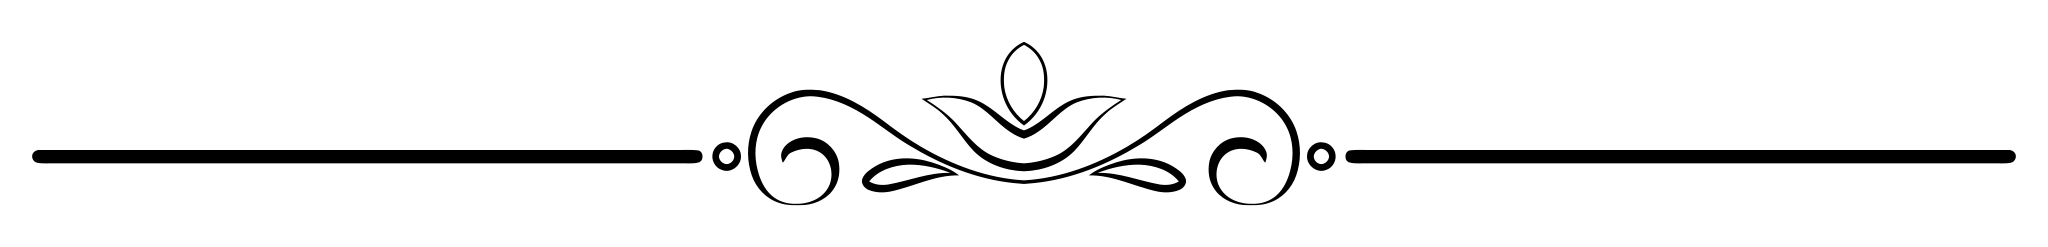
\includegraphics{images/Elegant-Flourish-Frame-Extrapolated-19.svg}

\newpage

This puzzle certainly has many possible answers. For all of them,
understanding what the regular expression is doing is the crucial
element. The short pattern might look odd, and you need to figure it
out. Here is a possibility.

\begin{Shaded}
\begin{Highlighting}[]
\KeywordTok{def}\NormalTok{ repeated\_prefix(s):}
    \CommentTok{"""Look for any prefix string in \textquotesingle{}s\textquotesingle{} and match only if}
\CommentTok{    that prefix is repeated at least once, but it might be}
\CommentTok{    repeated many times.  No other substring may occur}
\CommentTok{    between the start and end of the string for a match.}
\CommentTok{    """}
    \ControlFlowTok{return} \KeywordTok{not}\NormalTok{ re.match(}\VerbatimStringTok{r\textquotesingle{}\^{}(.+?)\textbackslash{}1+$\textquotesingle{}}\NormalTok{, s)}
\end{Highlighting}
\end{Shaded}

\begin{figure}
\centering
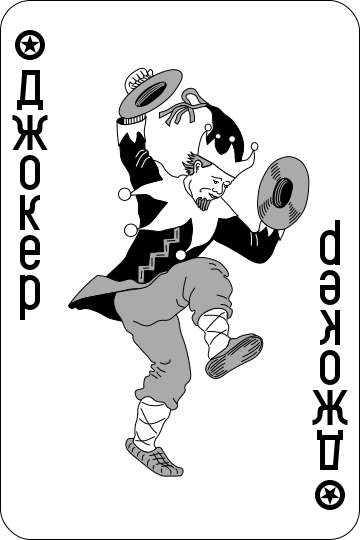
\includegraphics{images/Atlas_deck_joker_black.svg}
\caption{Atlas\_deck\_joker\_black}
\end{figure}

\newpage

\hypertarget{playing-poker-part-1}{%
\section{Playing Poker (Part 1)}\label{playing-poker-part-1}}

In earlier puzzles, we had fun playing dominoes. For the next few
puzzles, let's play poker. In particular, let's say that a player has
five cards, and we wish to compare two hands to each other. We will do
this, over several puzzles, by building up small functions to answer
various questions.

As much as possible, you should use regular expressions to express the
logic; however, a few of the questions will require a little bit of
non-regex code as well. First, let's remind ourselves of the ranking of
different hands of 5 cards. Our encoding will simplify card
representations a little bit. Specifically, the card that might be
called, e.g., \texttt{10♥} will be called \texttt{T♥} so that every card
is a two symbol combination.

\begin{itemize}
\tightlist
\item
  Straight flush, e.g.~\texttt{J♣\ T♣\ 9♣\ 8♣\ 7♣}
\item
  Four of a kind, e.g.~\texttt{A♥\ 3♠\ 3♥\ 3♦\ 3♣}
\item
  Full house, e.g.~\texttt{K♠\ K♣\ 6♥\ 6♦\ 6♣}
\item
  Flush, e.g.~\texttt{J♦\ 9♦\ 6♦\ 5♦\ 2♦}
\item
  Straight, e.g.~\texttt{9♦\ 8♣\ 7♣\ 6♥\ 5♣}
\item
  Three of a kind, e.g.~\texttt{Q♣\ 8♠\ 8♦\ 8♣\ 3♥}
\item
  Two pairs, e.g.~\texttt{J♠\ J♣\ 9♥\ 8♥\ 8♦}
\item
  One pair, e.g.~\texttt{A♥\ K♦\ 4♠\ 4♥\ 3♠}
\item
  High card, e.g.~\texttt{K♠\ 9♥\ 8♠\ 4♥\ 2♣}
\end{itemize}

Within the same kind of hand, other rules come into play. Let's ignore
those for now. We'd like two support functions to start. First, you
should write a function \texttt{prettify(hand)} that takes an
easier-to-type representation of suits as `S', `H', `D', `C', and turns
the hands into their Unicode symbols.

\newpage

The second and more difficult function for this puzzle asks you to make
sure all the cards are sorted in descending order (as in the examples),
where aces are always considered high, and the suits are ordered spades,
hearts, diamonds, clubs.

This second function, \texttt{cardsort(hand)}, uses more Python than
regular expressions per se, so just read the solution if you are less
comfortable with Python itself.

Before you turn the page\ldots{}

\textbf{Functions are a big help in larger programs.}

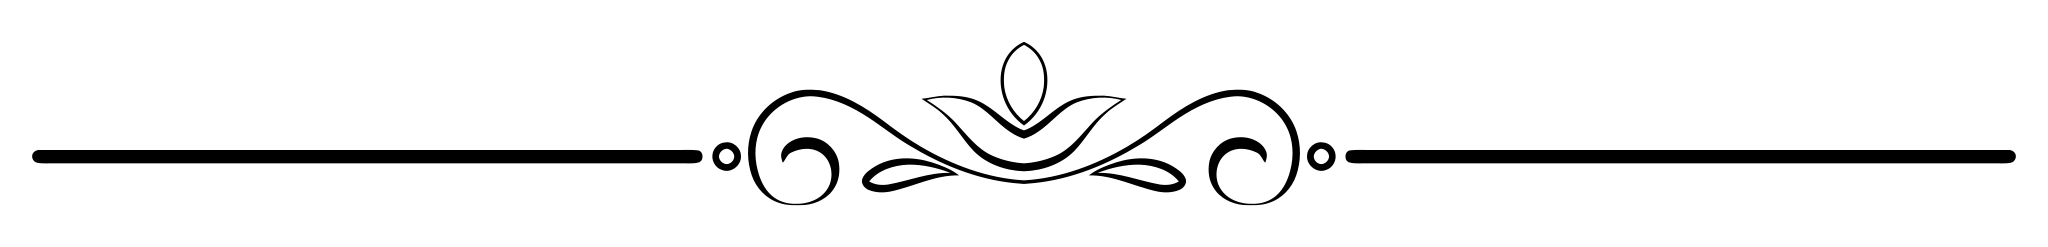
\includegraphics{images/Elegant-Flourish-Frame-Extrapolated-19.svg}

\newpage

The truth is, we do not genuinely \emph{need} regular expressions for
either of these support functions. But we do have the opportunity to use
them. First let's transform any ASCII version of a hand into the Unicode
version. Along the way, we make sure the hand consists of five valid
ASCII cards.

\begin{Shaded}
\begin{Highlighting}[]
\KeywordTok{def}\NormalTok{ prettify(hand):}
    \ControlFlowTok{assert}\NormalTok{ re.search(}\VerbatimStringTok{r\textquotesingle{}\^{}([2{-}9TJQKA][SHDC] ?)}\SpecialCharTok{\{5\}}\VerbatimStringTok{$\textquotesingle{}}\NormalTok{, hand)}
\NormalTok{    symbols }\OperatorTok{=}\NormalTok{ \{}\StringTok{\textquotesingle{}S\textquotesingle{}}\NormalTok{: }\StringTok{\textquotesingle{}}\CharTok{\textbackslash{}u2660}\StringTok{\textquotesingle{}}\NormalTok{, }\StringTok{\textquotesingle{}H\textquotesingle{}}\NormalTok{: }\StringTok{\textquotesingle{}}\CharTok{\textbackslash{}u2665}\StringTok{\textquotesingle{}}\NormalTok{,}
               \StringTok{\textquotesingle{}D\textquotesingle{}}\NormalTok{: }\StringTok{\textquotesingle{}}\CharTok{\textbackslash{}u2666}\StringTok{\textquotesingle{}}\NormalTok{, }\StringTok{\textquotesingle{}C\textquotesingle{}}\NormalTok{: }\StringTok{\textquotesingle{}}\CharTok{\textbackslash{}u2663}\StringTok{\textquotesingle{}}\NormalTok{\}}
    \ControlFlowTok{for}\NormalTok{ let, suit }\KeywordTok{in}\NormalTok{ symbols.items():}
\NormalTok{        hand }\OperatorTok{=}\NormalTok{ re.sub(let, suit, hand)}
    \ControlFlowTok{return}\NormalTok{ hand}
\end{Highlighting}
\end{Shaded}

Sorting uses mostly plain Python techniques. In particular, we can rely
on the fact that Python's sort is \emph{stable}. This means the order
will not change between equivalent elements. Therefore, sorting first by
suit, then by number will be guaranteed to have the right overall
effect.

\begin{Shaded}
\begin{Highlighting}[]
\KeywordTok{def}\NormalTok{ cardsort(hand):}
    \KeywordTok{def}\NormalTok{ by\_num(card):}
        \BuiltInTok{map} \OperatorTok{=}\NormalTok{ \{}\StringTok{\textquotesingle{}T\textquotesingle{}}\NormalTok{:}\StringTok{\textquotesingle{}A\textquotesingle{}}\NormalTok{, }\StringTok{\textquotesingle{}J\textquotesingle{}}\NormalTok{:}\StringTok{\textquotesingle{}B\textquotesingle{}}\NormalTok{, }\StringTok{\textquotesingle{}Q\textquotesingle{}}\NormalTok{:}\StringTok{\textquotesingle{}C\textquotesingle{}}\NormalTok{,}
               \StringTok{\textquotesingle{}K\textquotesingle{}}\NormalTok{:}\StringTok{\textquotesingle{}D\textquotesingle{}}\NormalTok{, }\StringTok{\textquotesingle{}A\textquotesingle{}}\NormalTok{:}\StringTok{\textquotesingle{}E\textquotesingle{}}\NormalTok{\}}
\NormalTok{        num }\OperatorTok{=}\NormalTok{ card[}\DecValTok{0}\NormalTok{]}
        \ControlFlowTok{return}\NormalTok{ num }\ControlFlowTok{if}\NormalTok{ num }\KeywordTok{not} \KeywordTok{in} \StringTok{\textquotesingle{}AKQJT\textquotesingle{}} \ControlFlowTok{else} \BuiltInTok{map}\NormalTok{[num]}

    \KeywordTok{def}\NormalTok{ by\_suit(card):}
        \BuiltInTok{map} \OperatorTok{=}\NormalTok{ \{}\StringTok{\textquotesingle{}}\CharTok{\textbackslash{}u2663}\StringTok{\textquotesingle{}}\NormalTok{: }\DecValTok{1}\NormalTok{, }\StringTok{\textquotesingle{}}\CharTok{\textbackslash{}u2666}\StringTok{\textquotesingle{}}\NormalTok{: }\DecValTok{2}\NormalTok{,}
               \StringTok{\textquotesingle{}}\CharTok{\textbackslash{}u2665}\StringTok{\textquotesingle{}}\NormalTok{: }\DecValTok{3}\NormalTok{, }\StringTok{\textquotesingle{}}\CharTok{\textbackslash{}u2660}\StringTok{\textquotesingle{}}\NormalTok{: }\DecValTok{4}\NormalTok{\}}
        \ControlFlowTok{return} \BuiltInTok{map}\NormalTok{[card[}\DecValTok{1}\NormalTok{]]}

\NormalTok{    hand }\OperatorTok{=}\NormalTok{ re.split(}\StringTok{\textquotesingle{} \textquotesingle{}}\NormalTok{, hand)}
\NormalTok{    hand.sort(key}\OperatorTok{=}\NormalTok{by\_suit, reverse}\OperatorTok{=}\VariableTok{True}\NormalTok{)}
\NormalTok{    hand.sort(key}\OperatorTok{=}\NormalTok{by\_num, reverse}\OperatorTok{=}\VariableTok{True}\NormalTok{)}
    \ControlFlowTok{return} \StringTok{\textquotesingle{} \textquotesingle{}}\NormalTok{.join(hand)}
\end{Highlighting}
\end{Shaded}

\newpage

Combining these:

\begin{Shaded}
\begin{Highlighting}[]
\OperatorTok{\textgreater{}\textgreater{}\textgreater{}}\NormalTok{ cardsort(prettify(}\StringTok{\textquotesingle{}8C AS 4H KS 2C\textquotesingle{}}\NormalTok{))}
\CommentTok{\textquotesingle{}A♠ K♠ 8♣ 4♥ 2♣\textquotesingle{}}
\end{Highlighting}
\end{Shaded}

We will need more regular expressions in the next few puzzles which
continue this poker theme.

\begin{figure}
\centering
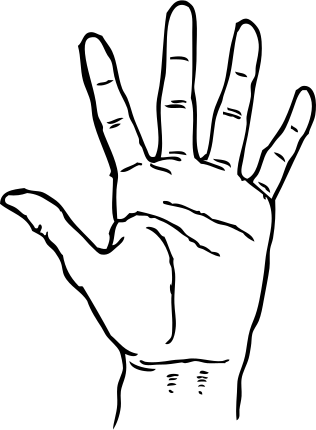
\includegraphics{images/johnny-automatic-left-hand-spread.svg}
\caption{johnny-automatic-left-hand-spread}
\end{figure}

\newpage

\hypertarget{playing-poker-part-2}{%
\section{Playing Poker (Part 2)}\label{playing-poker-part-2}}

In the last puzzle, you converted ``poker hands'' from ASCII to Unicode
suit symbols, and you also made sure that hands are listed in canonical
descending card order.

For this puzzle, you want to start using regular expressions to figure
out whether hands belong to various kinds. Here's an obvious trick we
can use as a shortcut:

\begin{Shaded}
\begin{Highlighting}[]
\KeywordTok{def}\NormalTok{ is\_straight\_flush(hand):}
    \ControlFlowTok{return}\NormalTok{ is\_straight(hand) }\KeywordTok{and}\NormalTok{ is\_flush(hand)}
\end{Highlighting}
\end{Shaded}

For this puzzle, you wish to write the functions
\texttt{is\_flush(hand)} and \texttt{is\_straight(hand)}, continuing
with the assumption that hands are represented in the same manner as the
last puzzle (including the cards being in descending order). Feel free
to use the \texttt{prettify()} function you wrote if it makes entering
test cases easier.

Before you turn the page\ldots{}

\textbf{Large buildings are built from small bricks.}

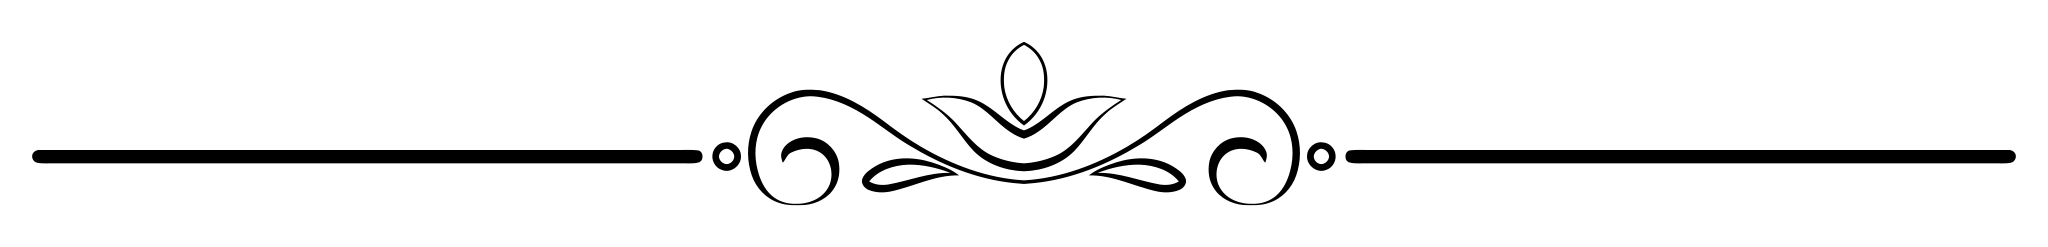
\includegraphics{images/Elegant-Flourish-Frame-Extrapolated-19.svg}

\newpage

Identifying a flush is somewhat easier. Moreover, if we are clever, we
can add two features to the function not specifically required in the
puzzle. We can make it work identically with the ASCII codes like `S'
for spaces and `H' for hearts simultaneously with the Unicode special
symbols.

But while we are creating the function, we can also return extra
``truthy'' information in the return value. Namely, if it \emph{is} a
flush, let's return the suit also.

\begin{Shaded}
\begin{Highlighting}[]
\OperatorTok{\textgreater{}\textgreater{}\textgreater{}} \KeywordTok{def}\NormalTok{ is\_flush(hand):}
\NormalTok{...     match }\OperatorTok{=}\NormalTok{ re.search(}\VerbatimStringTok{r\textquotesingle{}\^{}.(.)(.*\textbackslash{}1)}\SpecialCharTok{\{4\}}\VerbatimStringTok{$\textquotesingle{}}\NormalTok{, hand)}
\NormalTok{...     }\ControlFlowTok{return}\NormalTok{ match.group(}\DecValTok{1}\NormalTok{) }\ControlFlowTok{if}\NormalTok{ match }\ControlFlowTok{else} \VariableTok{False}

\OperatorTok{\textgreater{}\textgreater{}\textgreater{}}\NormalTok{ is\_flush(}\StringTok{\textquotesingle{}J♣ T♣ 9♣ 8♣ 7♣\textquotesingle{}}\NormalTok{)}
\CommentTok{\textquotesingle{}♣\textquotesingle{}}
\OperatorTok{\textgreater{}\textgreater{}\textgreater{}}\NormalTok{ is\_flush(}\StringTok{\textquotesingle{}J♦ 9♦ 6♦ 5♦ 2♦\textquotesingle{}}\NormalTok{)}
\CommentTok{\textquotesingle{}♦\textquotesingle{}}
\OperatorTok{\textgreater{}\textgreater{}\textgreater{}}\NormalTok{ is\_flush(}\StringTok{\textquotesingle{}J♦ 9♥ 6♦ 5♦ 2♦\textquotesingle{}}\NormalTok{)}
\VariableTok{False}
\OperatorTok{\textgreater{}\textgreater{}\textgreater{}}\NormalTok{ is\_flush(}\StringTok{\textquotesingle{}JD 9H 6D 5D 2D\textquotesingle{}}\NormalTok{)}
\VariableTok{False}
\OperatorTok{\textgreater{}\textgreater{}\textgreater{}}\NormalTok{ is\_flush(}\StringTok{\textquotesingle{}JD 9D 6D 5D 2D\textquotesingle{}}\NormalTok{)}
\CommentTok{\textquotesingle{}D\textquotesingle{}}
\end{Highlighting}
\end{Shaded}

For checking for straights, let's add a similar bit of extra information
in the return value. Obviously, if the hand is not a straight, we should
return False. But if it is one, we can return the high card number for
later use. Those are all ``truthy'' values (like all strings).

\begin{Shaded}
\begin{Highlighting}[]
\OperatorTok{\textgreater{}\textgreater{}\textgreater{}} \KeywordTok{def}\NormalTok{ is\_straight(hand):}
\NormalTok{...     pat }\OperatorTok{=} \VerbatimStringTok{r\textquotesingle{}[ SHDC\textbackslash{}u2660\textbackslash{}u2665\textbackslash{}u2666\textbackslash{}u2663]\textquotesingle{}}
\NormalTok{...     h }\OperatorTok{=}\NormalTok{ re.sub(pat, }\StringTok{\textquotesingle{}\textquotesingle{}}\NormalTok{, hand)}
\NormalTok{...     match }\OperatorTok{=}\NormalTok{ re.search(h, }\StringTok{\textquotesingle{}AKQJT98765432\textquotesingle{}}\NormalTok{) }
\NormalTok{...     }\ControlFlowTok{return}\NormalTok{ h[}\DecValTok{0}\NormalTok{] }\ControlFlowTok{if}\NormalTok{ match }\ControlFlowTok{else} \VariableTok{False}
\end{Highlighting}
\end{Shaded}

As with the first function, we might as well be friendly in accepting
the ASCII version of suits, even though they could always be improved
with \texttt{prettify()} if necessary. The pattern looks for everything
that is a suit character or a space, and strips it out to create a
simplified ``hand.''

\newpage

With the simplified hand of just ``numbers,'' we know that any straight
must be a substring of the run of all numbers. We do not check again
that the length is 5, trusting that other functions have validated this.
We could easily add that if we wanted, of course.

At this point, you might consider a richer implementation of
\texttt{is\_straight\_flush()}. Perhaps this:

\begin{Shaded}
\begin{Highlighting}[]
\OperatorTok{\textgreater{}\textgreater{}\textgreater{}} \KeywordTok{def}\NormalTok{ is\_straight\_flush(hand):}
\NormalTok{...     s }\OperatorTok{=}\NormalTok{ is\_straight(hand)}
\NormalTok{...     f }\OperatorTok{=}\NormalTok{ is\_flush(hand)}
\NormalTok{...     }\ControlFlowTok{return}\NormalTok{ s}\OperatorTok{+}\NormalTok{f }\ControlFlowTok{if}\NormalTok{ s }\KeywordTok{and}\NormalTok{ f }\ControlFlowTok{else} \VariableTok{False}

\OperatorTok{\textgreater{}\textgreater{}\textgreater{}}\NormalTok{ is\_straight\_flush(}\StringTok{\textquotesingle{}JD TD 9D 8D 7D\textquotesingle{}}\NormalTok{)}
\CommentTok{\textquotesingle{}JD\textquotesingle{}}
\OperatorTok{\textgreater{}\textgreater{}\textgreater{}}\NormalTok{ is\_straight\_flush(}\StringTok{\textquotesingle{}JD TD 9H 8D 7D\textquotesingle{}}\NormalTok{)}
\VariableTok{False}
\end{Highlighting}
\end{Shaded}

\begin{figure}
\centering
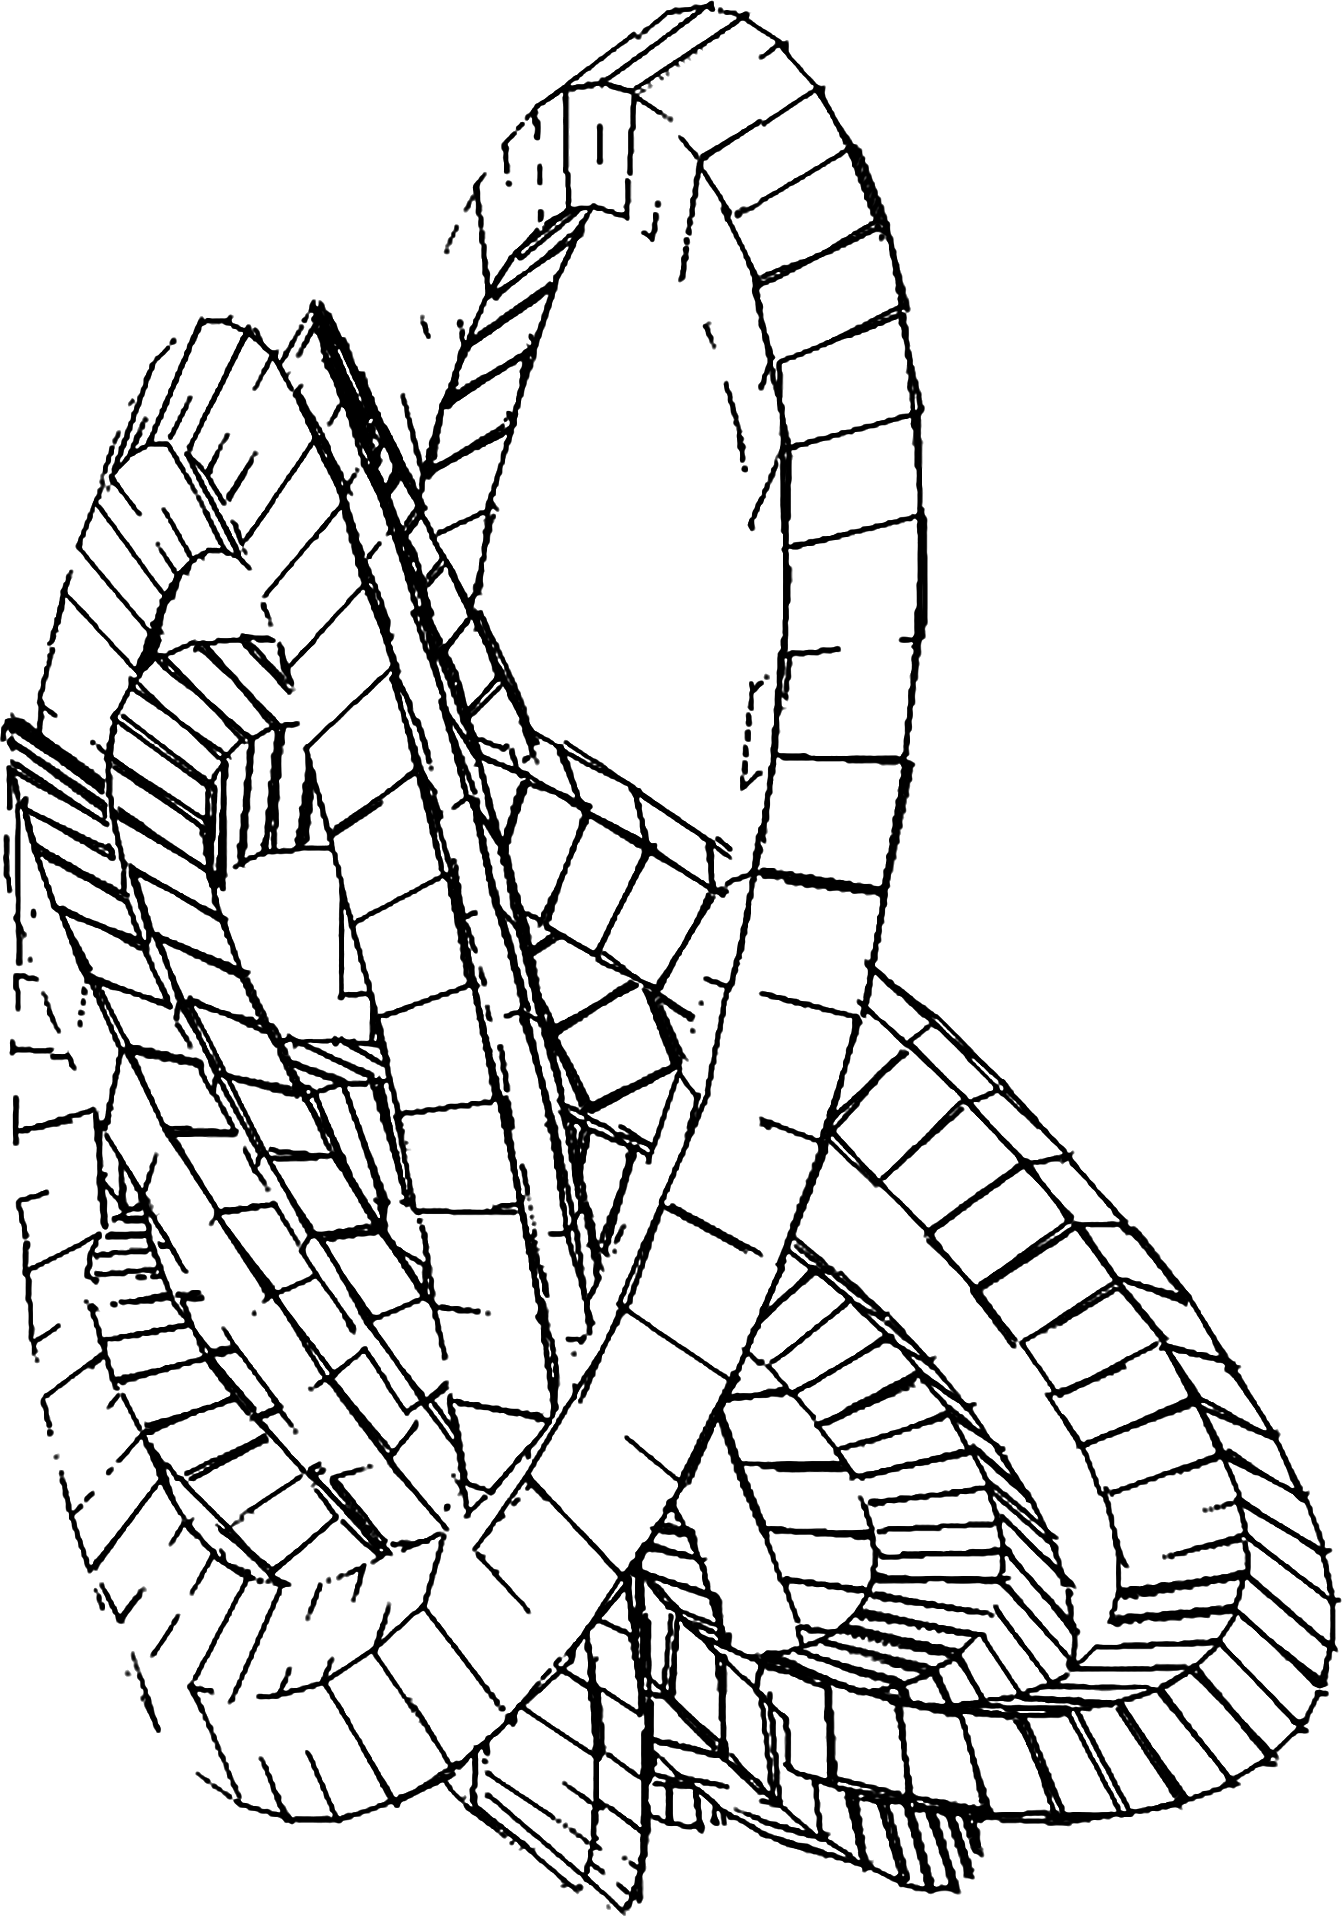
\includegraphics{images/Basket_Verso.png}
\caption{Basket\_Verso}
\end{figure}

\newpage

\hypertarget{playing-poker-part-3}{%
\section{Playing Poker (Part 3)}\label{playing-poker-part-3}}

In this puzzle let's continue with matching poker hands. We handled
straights and flushes in the last puzzle (and straight flushes by
obvious combination). There are some other types of hands to consider
now.

The next several types of hand have containing relationships among them.
That is, just like a straight flush is both a straight and a flush,
four-of-a-kind is trivially also three-of-a-kind and a pair. A full
house is both three-of-a-kind and a pair. However, for our purposes, we
will simply assume the various tests are performed in appropriate
descending order of strength. The first successful test will be the
classified type of the hand.

For the next few puzzles, therefore, write these functions:

\begin{itemize}
\tightlist
\item
  \texttt{is\_four\_of\_kind(hand)}
\item
  \texttt{is\_full\_house(hand)}
\item
  \texttt{is\_three\_of\_kind(hand)}
\item
  \texttt{is\_two\_pairs(hand)}
\item
  \texttt{is\_pair()}
\end{itemize}

This and the next few puzzles cover the various functions. See if you
can solve all of them (possibly using shared functionality) before
looking at the discussion.

Before you turn the page\ldots{}

\textbf{You better cheat, cheat, if you can't win.}

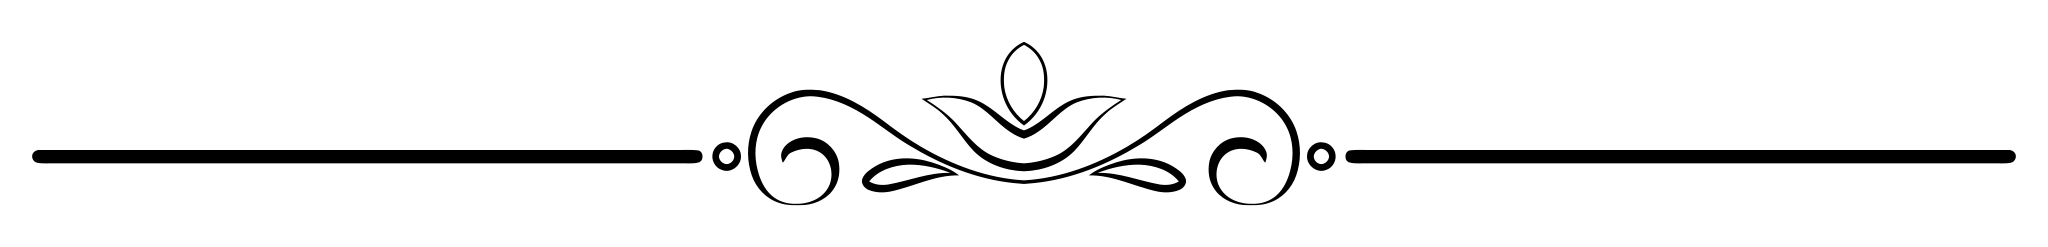
\includegraphics{images/Elegant-Flourish-Frame-Extrapolated-19.svg}

\newpage

If we have a four-of-a-kind, then the kind must occur in either the
first or second card. In fact, if we retain our assumption that the
cards are completely ordered, then the four can only occur as the
initial four or the final four. But the following implementation does
not rely on that ordering:

\begin{Shaded}
\begin{Highlighting}[]
\OperatorTok{\textgreater{}\textgreater{}} \KeywordTok{def}\NormalTok{ is\_four\_of\_kind(hand):}
\NormalTok{...     hand }\OperatorTok{=}\NormalTok{ re.sub(}\VerbatimStringTok{r\textquotesingle{}[\^{}AKQJT98765432]\textquotesingle{}}\NormalTok{, }\StringTok{\textquotesingle{}\textquotesingle{}}\NormalTok{, hand)}
\NormalTok{...     pat }\OperatorTok{=} \VerbatimStringTok{r\textquotesingle{}\^{}.?(.)(.*\textbackslash{}1)}\SpecialCharTok{\{3\}}\VerbatimStringTok{\textquotesingle{}}
\NormalTok{...     match }\OperatorTok{=}\NormalTok{ re.search(pat, hand)}
\NormalTok{...     }\CommentTok{\# Return the card number as truthy value}
\NormalTok{...     }\ControlFlowTok{return}\NormalTok{ match.group(}\DecValTok{1}\NormalTok{) }\ControlFlowTok{if}\NormalTok{ match }\ControlFlowTok{else} \VariableTok{False}
\NormalTok{...}
\OperatorTok{\textgreater{}\textgreater{}\textgreater{}}\NormalTok{ is\_four\_of\_kind(}\StringTok{\textquotesingle{}6H 6D 6S 6C 3S\textquotesingle{}}\NormalTok{) }\CommentTok{\# sorted}
\CommentTok{\textquotesingle{}6\textquotesingle{}}
\OperatorTok{\textgreater{}\textgreater{}\textgreater{}}\NormalTok{ is\_four\_of\_kind(}\StringTok{\textquotesingle{}6♦ 3♠ 6♥ 6♠ 6♣\textquotesingle{}}\NormalTok{) }\CommentTok{\# not sorted}
\CommentTok{\textquotesingle{}6\textquotesingle{}}
\OperatorTok{\textgreater{}\textgreater{}\textgreater{}}\NormalTok{ is\_four\_of\_kind(}\StringTok{\textquotesingle{}6H 6D 6S 4C 3S\textquotesingle{}}\NormalTok{) }\CommentTok{\# not four{-}of{-}kind}
\VariableTok{False}
\end{Highlighting}
\end{Shaded}

The first step is to remove everything that isn't a card number. Then we
either match nothing or the first character of the simplified hand. In
the zero-width case, the following group will get the number of the
first card. In the one-width case, the group will capture the second
card.

The group simply grabs one character, then we must find 3 more copies of
that group, but allow any prefix before each repetition. If we promised
that the hand was always ordered, the extra stuff before the
backreference would not be needed, but it does no harm in being zero
width.

\newpage

\hypertarget{playing-poker-part-4}{%
\section{Playing Poker (Part 4)}\label{playing-poker-part-4}}

Keeping in mind that we need only minimally identify each type of hand
within the corresponding function, not rule out other higher ranked
hands, we can take several different approaches to poker regexen.

Recall our possible hands:

\begin{itemize}
\tightlist
\item
  \texttt{is\_four\_of\_kind(hand)}
\item
  \texttt{is\_full\_house(hand)}
\item
  \texttt{is\_three\_of\_kind(hand)}
\item
  \texttt{is\_two\_pairs(hand)}
\item
  \texttt{is\_pair()}
\end{itemize}

Four-of-a-kind we did in the last puzzle, so now we want to deal with a
full house. Write a function, using regular expressions as much as
possible, to identify a hand that contains a full house.

Before you turn the page\ldots{}

\textbf{You might risk identifying the ``dead man's hand.''}

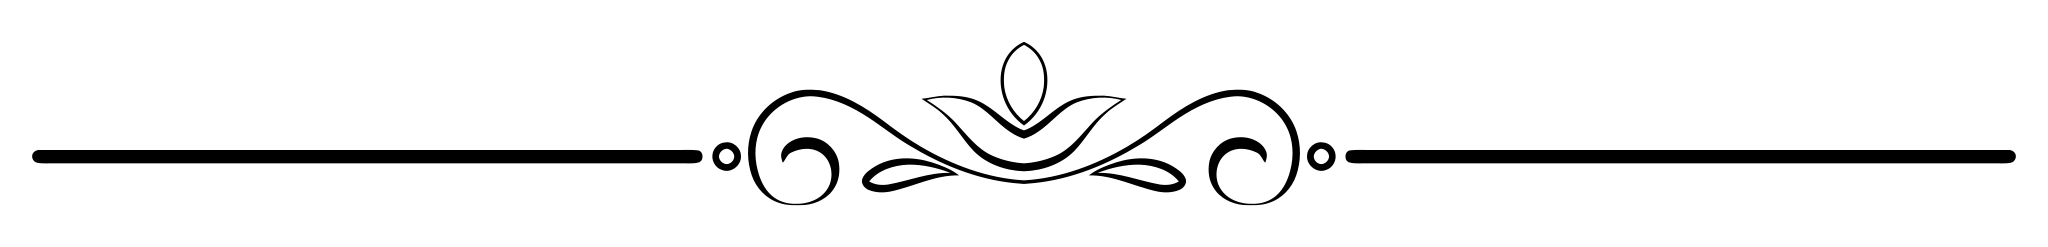
\includegraphics{images/Elegant-Flourish-Frame-Extrapolated-19.svg}

\newpage

One approach you might take for this puzzle is to identify both
\texttt{is\_three\_of\_kind()} and \texttt{is\_pair()} in the same hand.
Every full house will match those functions. However, in many of the
obvious implementations of those support functions, the two initial
cards that make up a triple would trigger \texttt{is\_pair()} even if
the last two cards are unmatched. There are ways to make that work, but
let's instead do it directly.

For this solution we use regular expressions to strip the suits, and
also to match the actual pattern. We can utilize the \texttt{cardsort()}
function, from Part 1 of the poker puzzles, to guarantee the hand is
sorted; we also make sure it is the ``pretty'' version rather than the
ASCII version since sorting assumes that.

The pattern itself is either two of the high number followed by three of
the low number, or three of the high number followed by two of the low
number. For later use, we can be extra nice by returning the 3-card
number first as the ``truthy'' value in a match. In most poker rules,
the 3-card match takes precedence when the same hands are evaluated for
the win.

\begin{Shaded}
\begin{Highlighting}[]
\OperatorTok{\textgreater{}\textgreater{}\textgreater{}} \KeywordTok{def}\NormalTok{ is\_full\_house(hand):}
\NormalTok{...     }\ControlFlowTok{try}\NormalTok{:}
\NormalTok{...         hand }\OperatorTok{=}\NormalTok{ prettify(hand)}
\NormalTok{...     }\ControlFlowTok{except}\NormalTok{:}
\NormalTok{...         }\ControlFlowTok{pass}  \CommentTok{\# Already pretty}
\NormalTok{...     hand }\OperatorTok{=}\NormalTok{ cardsort(hand)}
\NormalTok{...     hand }\OperatorTok{=}\NormalTok{ re.sub(}\VerbatimStringTok{r\textquotesingle{}[\^{}AKQJT98765432]\textquotesingle{}}\NormalTok{, }\StringTok{\textquotesingle{}\textquotesingle{}}\NormalTok{, hand)}
\NormalTok{...     }\CommentTok{\# Either three of suit then two of other, or}
\NormalTok{...     }\CommentTok{\# Two of suit then three of other}
\NormalTok{...     pat }\OperatorTok{=} \VerbatimStringTok{r"\^{}((.)\textbackslash{}2\{1,2\})((.)\textbackslash{}4\{1,2\})$"}
\NormalTok{...     match }\OperatorTok{=}\NormalTok{ re.search(pat, hand)}
\NormalTok{...     }\ControlFlowTok{if} \KeywordTok{not}\NormalTok{ match:}
\NormalTok{...         }\ControlFlowTok{return} \VariableTok{False}
\NormalTok{...     }\ControlFlowTok{elif} \BuiltInTok{len}\NormalTok{(match.group(}\DecValTok{3}\NormalTok{)) }\OperatorTok{\textgreater{}} \BuiltInTok{len}\NormalTok{(match.group(}\DecValTok{1}\NormalTok{)):}
\NormalTok{...         }\ControlFlowTok{return}\NormalTok{ hand[}\DecValTok{4}\NormalTok{] }\OperatorTok{+}\NormalTok{ hand [}\DecValTok{0}\NormalTok{]}
\NormalTok{...     }\ControlFlowTok{else}\NormalTok{:}
\NormalTok{...         }\ControlFlowTok{return}\NormalTok{ hand[}\DecValTok{0}\NormalTok{] }\OperatorTok{+}\NormalTok{ hand[}\DecValTok{4}\NormalTok{]}
\end{Highlighting}
\end{Shaded}

\newpage

\begin{Shaded}
\begin{Highlighting}[]
\OperatorTok{\textgreater{}\textgreater{}\textgreater{}}\NormalTok{ is\_full\_house(prettify(}\StringTok{\textquotesingle{}AS AC 8H 8D 8C\textquotesingle{}}\NormalTok{))}
\CommentTok{\textquotesingle{}8A\textquotesingle{}}
\OperatorTok{\textgreater{}\textgreater{}\textgreater{}}\NormalTok{ is\_full\_house(prettify(}\StringTok{\textquotesingle{}AS AH AC 8D 8C\textquotesingle{}}\NormalTok{))}
\CommentTok{\textquotesingle{}A8\textquotesingle{}}
\OperatorTok{\textgreater{}\textgreater{}\textgreater{}}\NormalTok{ is\_full\_house(prettify(}\StringTok{\textquotesingle{}AS AH JD 8D 8C\textquotesingle{}}\NormalTok{))}
\VariableTok{False}
\end{Highlighting}
\end{Shaded}

Obviously, this solution involves a moderate amount of non-regex Python.
But the heart of it is the same reduction to number-only we saw with
\texttt{is\_four\_of\_kind()} followed by the pattern described. The
just-Python part is really only to provide the friendly truthy values,
not in asking the predicate itself.

\begin{figure}
\centering
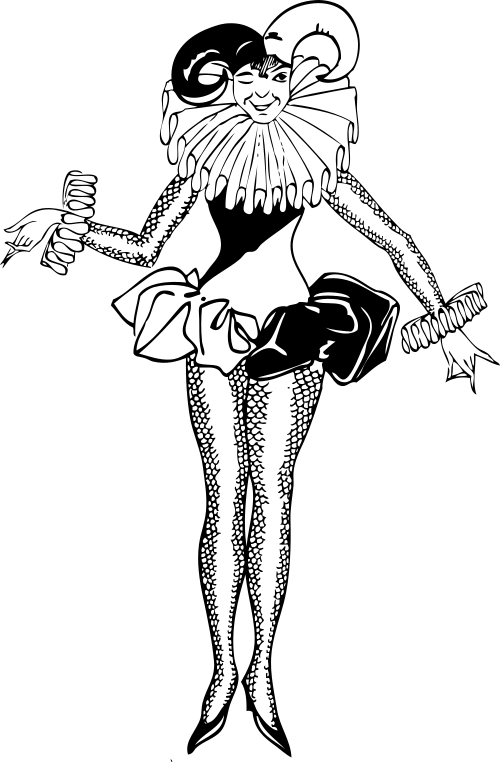
\includegraphics{images/clown-28772.svg}
\caption{clown-28772}
\end{figure}

\newpage

\hypertarget{playing-poker-part-5}{%
\section{Playing Poker (Part 5)}\label{playing-poker-part-5}}

In the last few puzzles we identified four-of-a-kind and full house.
Much of the logic for this puzzle will be similar to those, but
obviously tweaked somewhat for the next cases.

All you have left in our poker regex family is to identify
three-of-a-kind, a pair, and two pairs. As before, you may assume that
tests for various hands will run in descending order of strength. So,
for example, if your test for a pair will incidentally detect a hand
that has four-of-a-kind, that is not a problem since it indeed ipso
facto has a pair.

Create these three functions in this puzzle:

\begin{itemize}
\tightlist
\item
  \texttt{is\_three\_of\_kind(hand)}
\item
  \texttt{is\_two\_pairs(hand)}
\item
  \texttt{is\_pair()}
\end{itemize}

Before you turn the page\ldots{}

\textbf{Remember that three is more than two, but less than four.}

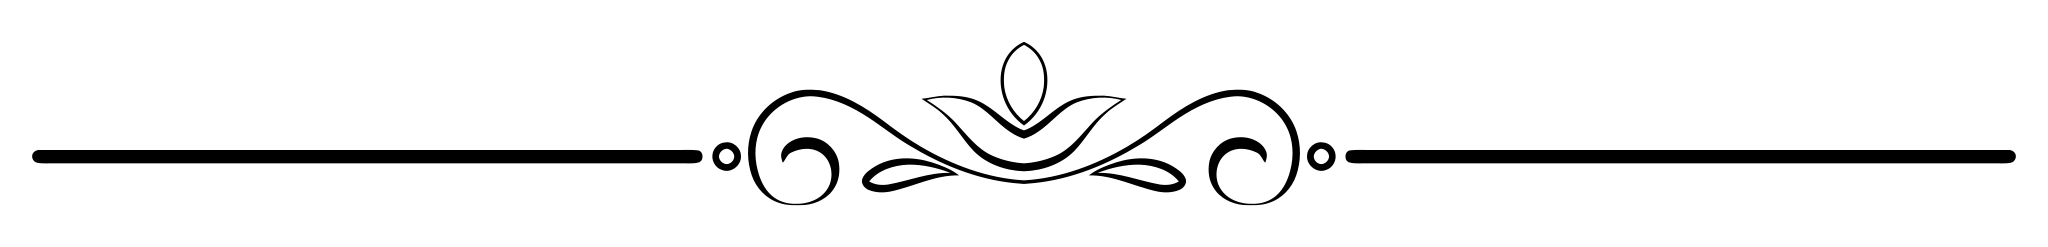
\includegraphics{images/Elegant-Flourish-Frame-Extrapolated-19.svg}

\newpage

Identifying two- or three-of-a-kind is a lot like identifying
four-of-a-kind, just with fewer repetitions. We could do it without
sorting the hand, but doing so, as with our full house solution, is a
bit easier.

\begin{Shaded}
\begin{Highlighting}[]
\OperatorTok{\textgreater{}\textgreater{}\textgreater{}} \KeywordTok{def}\NormalTok{ is\_three\_of\_kind(hand):}
\NormalTok{...     }\ControlFlowTok{try}\NormalTok{:}
\NormalTok{...         hand }\OperatorTok{=}\NormalTok{ prettify(hand)}
\NormalTok{...     }\ControlFlowTok{except}\NormalTok{:}
\NormalTok{...         }\ControlFlowTok{pass}  \CommentTok{\# Already pretty}
\NormalTok{...     hand }\OperatorTok{=}\NormalTok{ cardsort(hand)}
\NormalTok{...     hand }\OperatorTok{=}\NormalTok{ re.sub(}\VerbatimStringTok{r\textquotesingle{}[\^{}AKQJT98765432]\textquotesingle{}}\NormalTok{, }\StringTok{\textquotesingle{}\textquotesingle{}}\NormalTok{, hand)}
\NormalTok{...     pat }\OperatorTok{=} \VerbatimStringTok{r\textquotesingle{}(.)\textbackslash{}1}\SpecialCharTok{\{2\}}\VerbatimStringTok{\textquotesingle{}}  \CommentTok{\# No begin/end markers}
\NormalTok{...     match }\OperatorTok{=}\NormalTok{ re.search(pat, hand)}
\NormalTok{...     }\ControlFlowTok{return}\NormalTok{ match.group(}\DecValTok{1}\NormalTok{) }\ControlFlowTok{if}\NormalTok{ match }\ControlFlowTok{else} \VariableTok{False}
\NormalTok{...}
\NormalTok{...}
\OperatorTok{\textgreater{}\textgreater{}\textgreater{}}\NormalTok{ is\_three\_of\_kind(}\StringTok{\textquotesingle{}AS 6H QH 6S 2D\textquotesingle{}}\NormalTok{)}
\VariableTok{False}
\OperatorTok{\textgreater{}\textgreater{}\textgreater{}}\NormalTok{ is\_three\_of\_kind(}\StringTok{\textquotesingle{}AS 6H QH 6S 6D\textquotesingle{}}\NormalTok{)}
\CommentTok{\textquotesingle{}6\textquotesingle{}}
\end{Highlighting}
\end{Shaded}

Identifying a pair is basically identical. We simply need to settle for
one copy of a card number rather than two copies.

\begin{Shaded}
\begin{Highlighting}[]
\KeywordTok{def}\NormalTok{ is\_pair(hand):}
    \ControlFlowTok{try}\NormalTok{:}
\NormalTok{        hand }\OperatorTok{=}\NormalTok{ prettify(hand)}
    \ControlFlowTok{except}\NormalTok{:}
        \ControlFlowTok{pass}  \CommentTok{\# Already pretty}
\NormalTok{    hand }\OperatorTok{=}\NormalTok{ cardsort(hand)}
\NormalTok{    hand }\OperatorTok{=}\NormalTok{ re.sub(}\VerbatimStringTok{r\textquotesingle{}[\^{}AKQJT98765432]\textquotesingle{}}\NormalTok{, }\StringTok{\textquotesingle{}\textquotesingle{}}\NormalTok{, hand)}
\NormalTok{    pat }\OperatorTok{=} \VerbatimStringTok{r\textquotesingle{}(.)\textbackslash{}1\textquotesingle{}}  \CommentTok{\# No begin/end markers}
\NormalTok{    match }\OperatorTok{=}\NormalTok{ re.search(pat, hand)}
    \ControlFlowTok{return}\NormalTok{ match.group(}\DecValTok{1}\NormalTok{) }\ControlFlowTok{if}\NormalTok{ match }\ControlFlowTok{else} \VariableTok{False}
\end{Highlighting}
\end{Shaded}

Matching two pairs is actually a little trickier. Remember that for a
full house we matched either two of one number followed by three of the
other, or matched the reverse, three then two. However, the ``gap'' of
an unmatched number can occur in more different ways in this case.
Thinking about it, two pairs might look like any of the following (even
assuming sorting):

\newpage

\begin{itemize}
\tightlist
\item
  \texttt{X\ X\ \_\ Y\ Y}
\item
  \texttt{\_\ X\ X\ Y\ Y}
\item
  \texttt{X\ X\ Y\ Y\ \_}
\end{itemize}

The unmatched number cannot occur in sorted positions 2 or 4 since that
leaves only three cards to the other side of the unmatched number (and
we have stipulated sorted order of the hand).

As elsewhere, we return the helpful ``truthy'' value that might be used
later in comparing hands of the same type (namely, the two numbers of
the pairs, in sorted order).

\begin{Shaded}
\begin{Highlighting}[]
\OperatorTok{\textgreater{}\textgreater{}\textgreater{}} \KeywordTok{def}\NormalTok{ is\_two\_pairs(hand):}
\NormalTok{...     }\ControlFlowTok{try}\NormalTok{:}
\NormalTok{...         hand }\OperatorTok{=}\NormalTok{ prettify(hand)}
\NormalTok{...     }\ControlFlowTok{except}\NormalTok{:}
\NormalTok{...         }\ControlFlowTok{pass}  \CommentTok{\# Already pretty}
\NormalTok{...     hand }\OperatorTok{=}\NormalTok{ cardsort(hand)}
\NormalTok{...     hand }\OperatorTok{=}\NormalTok{ re.sub(}\VerbatimStringTok{r\textquotesingle{}[\^{}[AKQJT98765432]\textquotesingle{}}\NormalTok{, }\StringTok{\textquotesingle{}\textquotesingle{}}\NormalTok{, hand)}
\NormalTok{...     }\CommentTok{\# Three ways to match with unmatched number}
\NormalTok{...     pat }\OperatorTok{=}\NormalTok{ (}\VerbatimStringTok{r"(.)\textbackslash{}1.(.)\textbackslash{}2|"}
\NormalTok{...            }\VerbatimStringTok{r".(.)\textbackslash{}3(.)\textbackslash{}4|"}
\NormalTok{...            }\VerbatimStringTok{r"(.)\textbackslash{}5(.)\textbackslash{}6."}\NormalTok{)}
\NormalTok{...     match }\OperatorTok{=}\NormalTok{ re.search(pat, hand)}
\NormalTok{...     }\ControlFlowTok{if} \KeywordTok{not}\NormalTok{ match:}
\NormalTok{...         }\ControlFlowTok{return} \VariableTok{False}
\NormalTok{...     }\ControlFlowTok{else}\NormalTok{:}
\NormalTok{...         }\ControlFlowTok{return} \StringTok{\textquotesingle{}\textquotesingle{}}\NormalTok{.join(n }\ControlFlowTok{for}\NormalTok{ n }\KeywordTok{in}\NormalTok{ match.groups() }\ControlFlowTok{if}\NormalTok{ n)}
\NormalTok{...}
\OperatorTok{\textgreater{}\textgreater{}\textgreater{}}\NormalTok{ is\_two\_pairs(}\StringTok{\textquotesingle{}AH 6S 3H AD 6C\textquotesingle{}}\NormalTok{)}
\CommentTok{\textquotesingle{}A6\textquotesingle{}}
\OperatorTok{\textgreater{}\textgreater{}\textgreater{}}\NormalTok{ is\_two\_pairs(}\StringTok{\textquotesingle{}AH 6S 3H AD 3C\textquotesingle{}}\NormalTok{)}
\CommentTok{\textquotesingle{}A3\textquotesingle{}}
\OperatorTok{\textgreater{}\textgreater{}\textgreater{}}\NormalTok{ is\_two\_pairs(}\StringTok{\textquotesingle{}AH 6S 3H KD 3C\textquotesingle{}}\NormalTok{)}
\VariableTok{False}
\end{Highlighting}
\end{Shaded}

The remainder of your poker game program is left for a further exercise.
The rest of what you'd need to do won't have much to do with regular
expressions, simply usual program flow and data structures.

\begin{figure}
\centering

\includegraphics{images/Naive_Scribble_Verso.png}
\caption{Naive\_Scribble\_Verso}
\end{figure}

\hypertarget{easy-difficult-and-impossible-tasks}{%
\chapter{Easy, Difficult, and Impossible
Tasks}\label{easy-difficult-and-impossible-tasks}}

Some things are difficult or impossible with regular expressions, and
many are elegant and highly expressive. The puzzles in this section ask
you to think about which situation each puzzle describes.

\begin{figure}
\centering
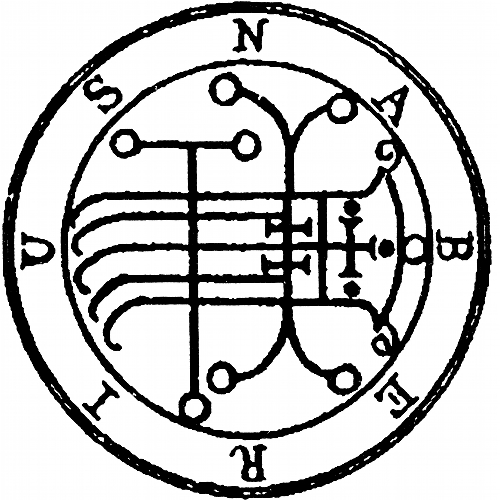
\includegraphics{images/N_A_B_E_R_I_U_S.jpg}
\caption{N\_A\_B\_E\_R\_I\_U\_S}
\end{figure}

\newpage

\hypertarget{identifying-equal-counts}{%
\section{Identifying Equal Counts}\label{identifying-equal-counts}}

At times we encounter a message or a stream that uses balanced
``increment'' and ``decrement'' symbols. For example, one way to check
that a message has terminated might be to match up the increments and
decrements. The same concept would apply to many kinds of messages and
symbols---perhaps you'd like to set the table with the same number of
forks and knives, for example.

As a simplification of the general problem, write a regular expression
that matches strings that consist of any number of `A' characters,
followed by the same number of `B' characters.

For example \texttt{AAABBB} and \texttt{AAAAAAABBBBBBB} should match,
while \texttt{AAAABBBBBB} should fail to match.

Before you turn the page\ldots{}

\textbf{Lateral thinking might help you find the answer.}

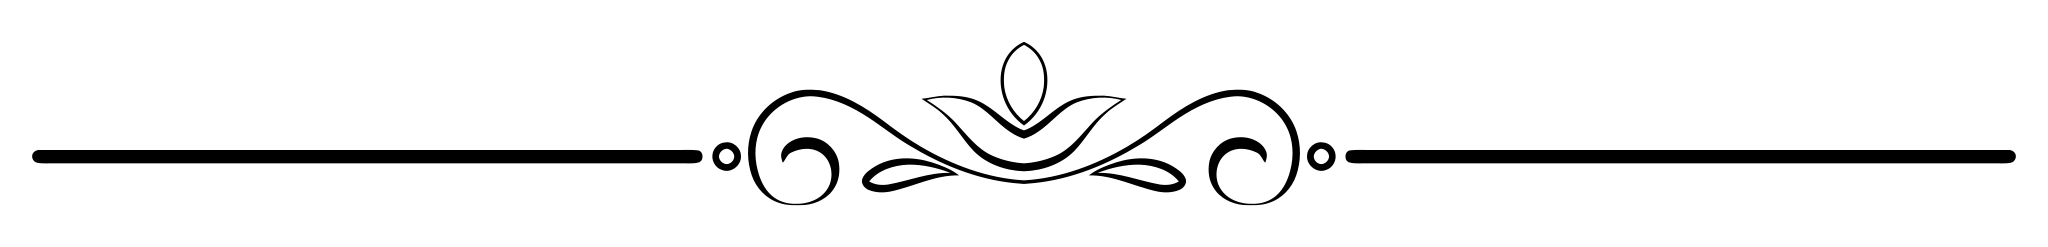
\includegraphics{images/Elegant-Flourish-Frame-Extrapolated-19.svg}

\newpage

You cannot match patterns based on having an equal number of different
symbols using regular expressions. Or at least you cannot do so in the
general case. It is, of course, perfectly possible to require exactly
seven 'A's and exactly seven 'B's. But if the count is arbitrarily
large, the kind of ``machine'' that can match the message requires
additional power.

In computer science or mathematical terms, a regular expression is
equivalet to a \emph{nondeterministic finite automaton} (NFA), where a
regex provides a very compact spelling of such an NFA. More powerful
machines include \emph{pushdown automata} (PDA) which have an
indefinitely large ``stack'' of stored symbols. One most often
encounters PDAs as parsers. A PDA, even the nondeterministic variety,
remains formally less powerful than a Turing Machine.

In simple terms, if you want to count occurrences, you need to use
variables that can store a number (or a data structure like a list to
hold the symbols).

Many new users of regexen fall into a trap of hoping this puzzle is
solvable. Or more often still, something equivalent like matching up
opening and closing parentheses, brackets, or XML/HTML tags. \emph{Hic
sunt dracones}! (Here be dragons)

\newpage

\hypertarget{matching-before-duplicate-words}{%
\section{Matching Before Duplicate
Words}\label{matching-before-duplicate-words}}

If you looked at the last puzzle, you saw that some match patterns you
might anticipate to be possible with regular expressions are actually
not expressible with regexen. Think about whether this puzzle is
possible and, if so, how.

Write a regular expression that will match all the initial words of a
string (including any punctuation or spacing that might surround words),
stopping before any word that is duplicated in the string. For example:

\begin{Shaded}
\begin{Highlighting}[]
\NormalTok{s1 }\OperatorTok{=} \StringTok{"this and that not other"}
\ControlFlowTok{assert}\NormalTok{ re.match(pat, s1).group() }\OperatorTok{==}\NormalTok{ s1}
\end{Highlighting}
\end{Shaded}

Remember that \texttt{re.match()} always starts at the beginning of a
string when looking for a match. If you preferred \texttt{re.search()}
you would need to begin the pattern with \texttt{\^{}}. In the first
example no word is duplicated in the phrase, and therefore the entire
phrase matches. In contrast:

\begin{Shaded}
\begin{Highlighting}[]
\NormalTok{s2 }\OperatorTok{=} \StringTok{"this and that and other"}
\ControlFlowTok{assert}\NormalTok{ re.match(pat, s2).group() }\OperatorTok{==} \StringTok{\textquotesingle{}this \textquotesingle{}}
\end{Highlighting}
\end{Shaded}

The second example is a little different. The first word `this' never
reoccurs. But the second word `and' does occur later in the phrase, and
therefore it, and everything following the duplicated word, must be
excluded.

Before you turn the page\ldots{}

\textbf{Find a pattern that will fulfill the requirment.}

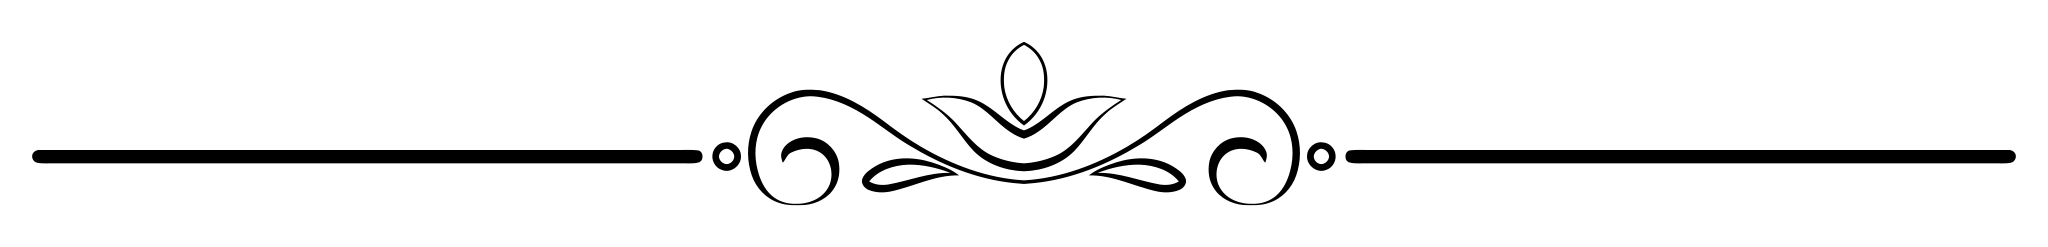
\includegraphics{images/Elegant-Flourish-Frame-Extrapolated-19.svg}

\newpage

This match pattern is indeed possible to write as a regular expression.
We need to use backreferences to check it, but those are a standard
feature of regular expression engines.

\begin{Shaded}
\begin{Highlighting}[]
\NormalTok{pat }\OperatorTok{=} \VerbatimStringTok{r\textquotesingle{}((\textbackslash{}w+\textbackslash{}b)(?!.*\textbackslash{}2\textbackslash{}b)\textbackslash{}W*)+\textquotesingle{}}
\end{Highlighting}
\end{Shaded}

As well as the backreference, we use a negative lookahead assertion.
That is, the basic thing being matched is
\texttt{(\textbackslash{}w+\textbackslash{}b)\textbackslash{}W*)+}. That
is to say, match one or more alphanumeric characters
\texttt{\textbackslash{}w} followed by a word boundary. That ``word''
might be followed by zero or more non-alphanumeric characters. Then
overall, match one or more repetitions of that general pattern.

So far, so good. But we have not excluded the repeated words. We do that
with the negative lookahead,
\texttt{(?!.*\textbackslash{}2\textbackslash{}b)}. That is, we want to
look through the entire rest of the string being evaluated, and make
sure that we do not encounter the same word currently matched. The
initial \texttt{.*} just matches any number of characters, but the
\texttt{\textbackslash{}2} is the actual current word. We still use word
boundary in the negative lookahead because a longer word of which the
current word is a prefix would be permitted.

Keep in mind how groups are numbered. Since there are parentheses
surrounding the entire expression (other than the \texttt{+}
quantifier), that whole thing is group 1. So the first subpattern inside
of that, matching the current word, is group 2, hence named as
\texttt{\textbackslash{}2}.

\newpage

\hypertarget{testing-an-ipv4-address}{%
\section{Testing an IPv4 Address}\label{testing-an-ipv4-address}}

``Internet protocol version 4'' addresses are prevalent in almost
everything we do with computers. ``Under the hood'' (so to speak), an
IPv4 address is just a 32-bit unsigned integer. However, it is universal
to write them in a human-memorable way as so-called dotted quads. In
that format, each byte of the address is represented as a decimal number
between 0 and 255 (the range of an integer byte), and the four bytes are
separated by periods.

Some particular address ranges have special or reserved meanings, but
they remain IPv4 addresses, and should be matched for this puzzle. Can
you write a regular expression to test if a string is a valid IPv4
address? Some examples:

\begin{itemize}
\tightlist
\item
  Valid: 192.168.20.1
\item
  Invalid: 292.168.10.1
\item
  Invalid: 5.138.0.21.23
\item
  Invalid: 192.AA.20.1
\end{itemize}

The first of these is a good address; it happens to be a range reserved
for internal addresses within an organization (usually one particular
router), and hence exists in many local networks. The others fail for
various reasons. The first invalid address contains numbers outside the
permitted integer range in one quad. The second invalid address has 5
dotted elements rather than 4. The third invalid address contains
characters other than decimal digits in one of the quads.

Before you turn the page\ldots{}

\textbf{Ask whether regexen are powerful enough for a problem.}

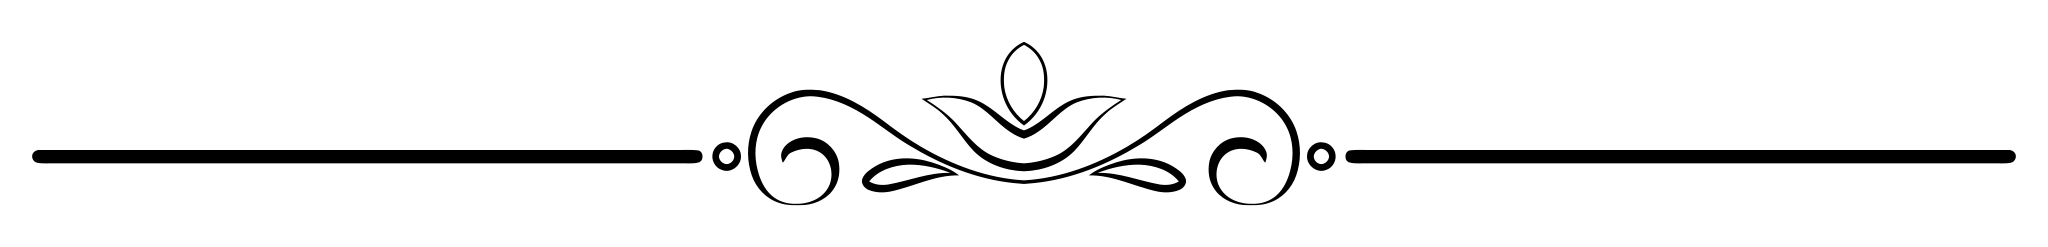
\includegraphics{images/Elegant-Flourish-Frame-Extrapolated-19.svg}

\newpage

It would be very easy to match naive \emph{dotted quads} that simply
consisted of four numbers with up to three digits, separated by dots.
You might express that as:

\begin{Shaded}
\begin{Highlighting}[]
\NormalTok{pat }\OperatorTok{=} \VerbatimStringTok{r\textquotesingle{}\^{}(\textbackslash{}d\{1{-}3\})}\SpecialCharTok{\{3\}}\VerbatimStringTok{\textbackslash{}.\textbackslash{}d\{1{-}3\}$\textquotesingle{}}
\end{Highlighting}
\end{Shaded}

This code will indeed match every IPv4 address. But it will also match
many things that are invalid, such as \texttt{992.0.100.13}. Matching
three-digit numbers that begin with 3-9 are definitely wrong. We can try
to fix that oversight by allowing only acceptable hundreds digits:

\begin{Shaded}
\begin{Highlighting}[]
\NormalTok{pat }\OperatorTok{=} \VerbatimStringTok{r\textquotesingle{}\^{}([12]?\textbackslash{}d\{1{-}2\})}\SpecialCharTok{\{3\}}\VerbatimStringTok{\textbackslash{}.[12]?\textbackslash{}d\{1{-}2\}$\textquotesingle{}}
\end{Highlighting}
\end{Shaded}

This has far fewer false positives. It says ``maybe start with a `1' or
a `2', then follow that by one or two more digits'' (repeating that for
dotted quads). So far, so good: \texttt{992.0.100.13} is ruled out. But
we still might accept \texttt{271.10.199.3} which has an invalid first
quad.

To fix the pattern we have to \emph{bite the bullet} and list all and
only quads we can allow. That is, if a quad starts with a `25' and has
three digits, the next digit can only be 0-5. And if it starts with a
`2' it definitely cannot have a digit more than 5 next.

\begin{Shaded}
\begin{Highlighting}[]
\NormalTok{pat }\OperatorTok{=}\NormalTok{ (}
    \StringTok{\textquotesingle{}\^{}((25[0{-}5]|2[0{-}4]\textbackslash{}d|[01]?\textbackslash{}d\textbackslash{}d?)\textbackslash{}.)}\SpecialCharTok{\{3\}}\StringTok{\textquotesingle{}}
      \StringTok{\textquotesingle{}(25[0{-}5]|2[0{-}4]\textbackslash{}d|[01]?\textbackslash{}d\textbackslash{}d?)$\textquotesingle{}}
\NormalTok{)}
\end{Highlighting}
\end{Shaded}

The pattern is a bit of a mouthful, but when we see how it is built up,
the pattern becomes quite clear and elegant. All the stuff after the
number quantifier \texttt{\{3\}} is just a repetition of the earlier
subpattern. This is simply because we match three numbers that are
followed by a period, but the final number must not be followed by
anything.

The main subpattern is just an alternation of options. Maybe the quad
looks like \texttt{25{[}0-5{]}}. Or maybe it looks like
\texttt{2{[}0-4{]}\textbackslash{}d}. These describe all the valid
numbers in the 200+ range. For the rest, we get a little clever.

If the quad isn't three digits beginning with a `2', it can either be
three-digits beginning with `1' or `0'. Conventionally, leading zeros
are dropped, but that is not required. However, two-digit or one-digit
numbers are also common; any such two- or one-digit numbers are
permitted. So we make the initial \texttt{{[}01{]}} optional, and also
make the final digit optional with \texttt{\textbackslash{}d?}. This
gives all and only the remaining permissible quads.

\begin{figure}
\centering
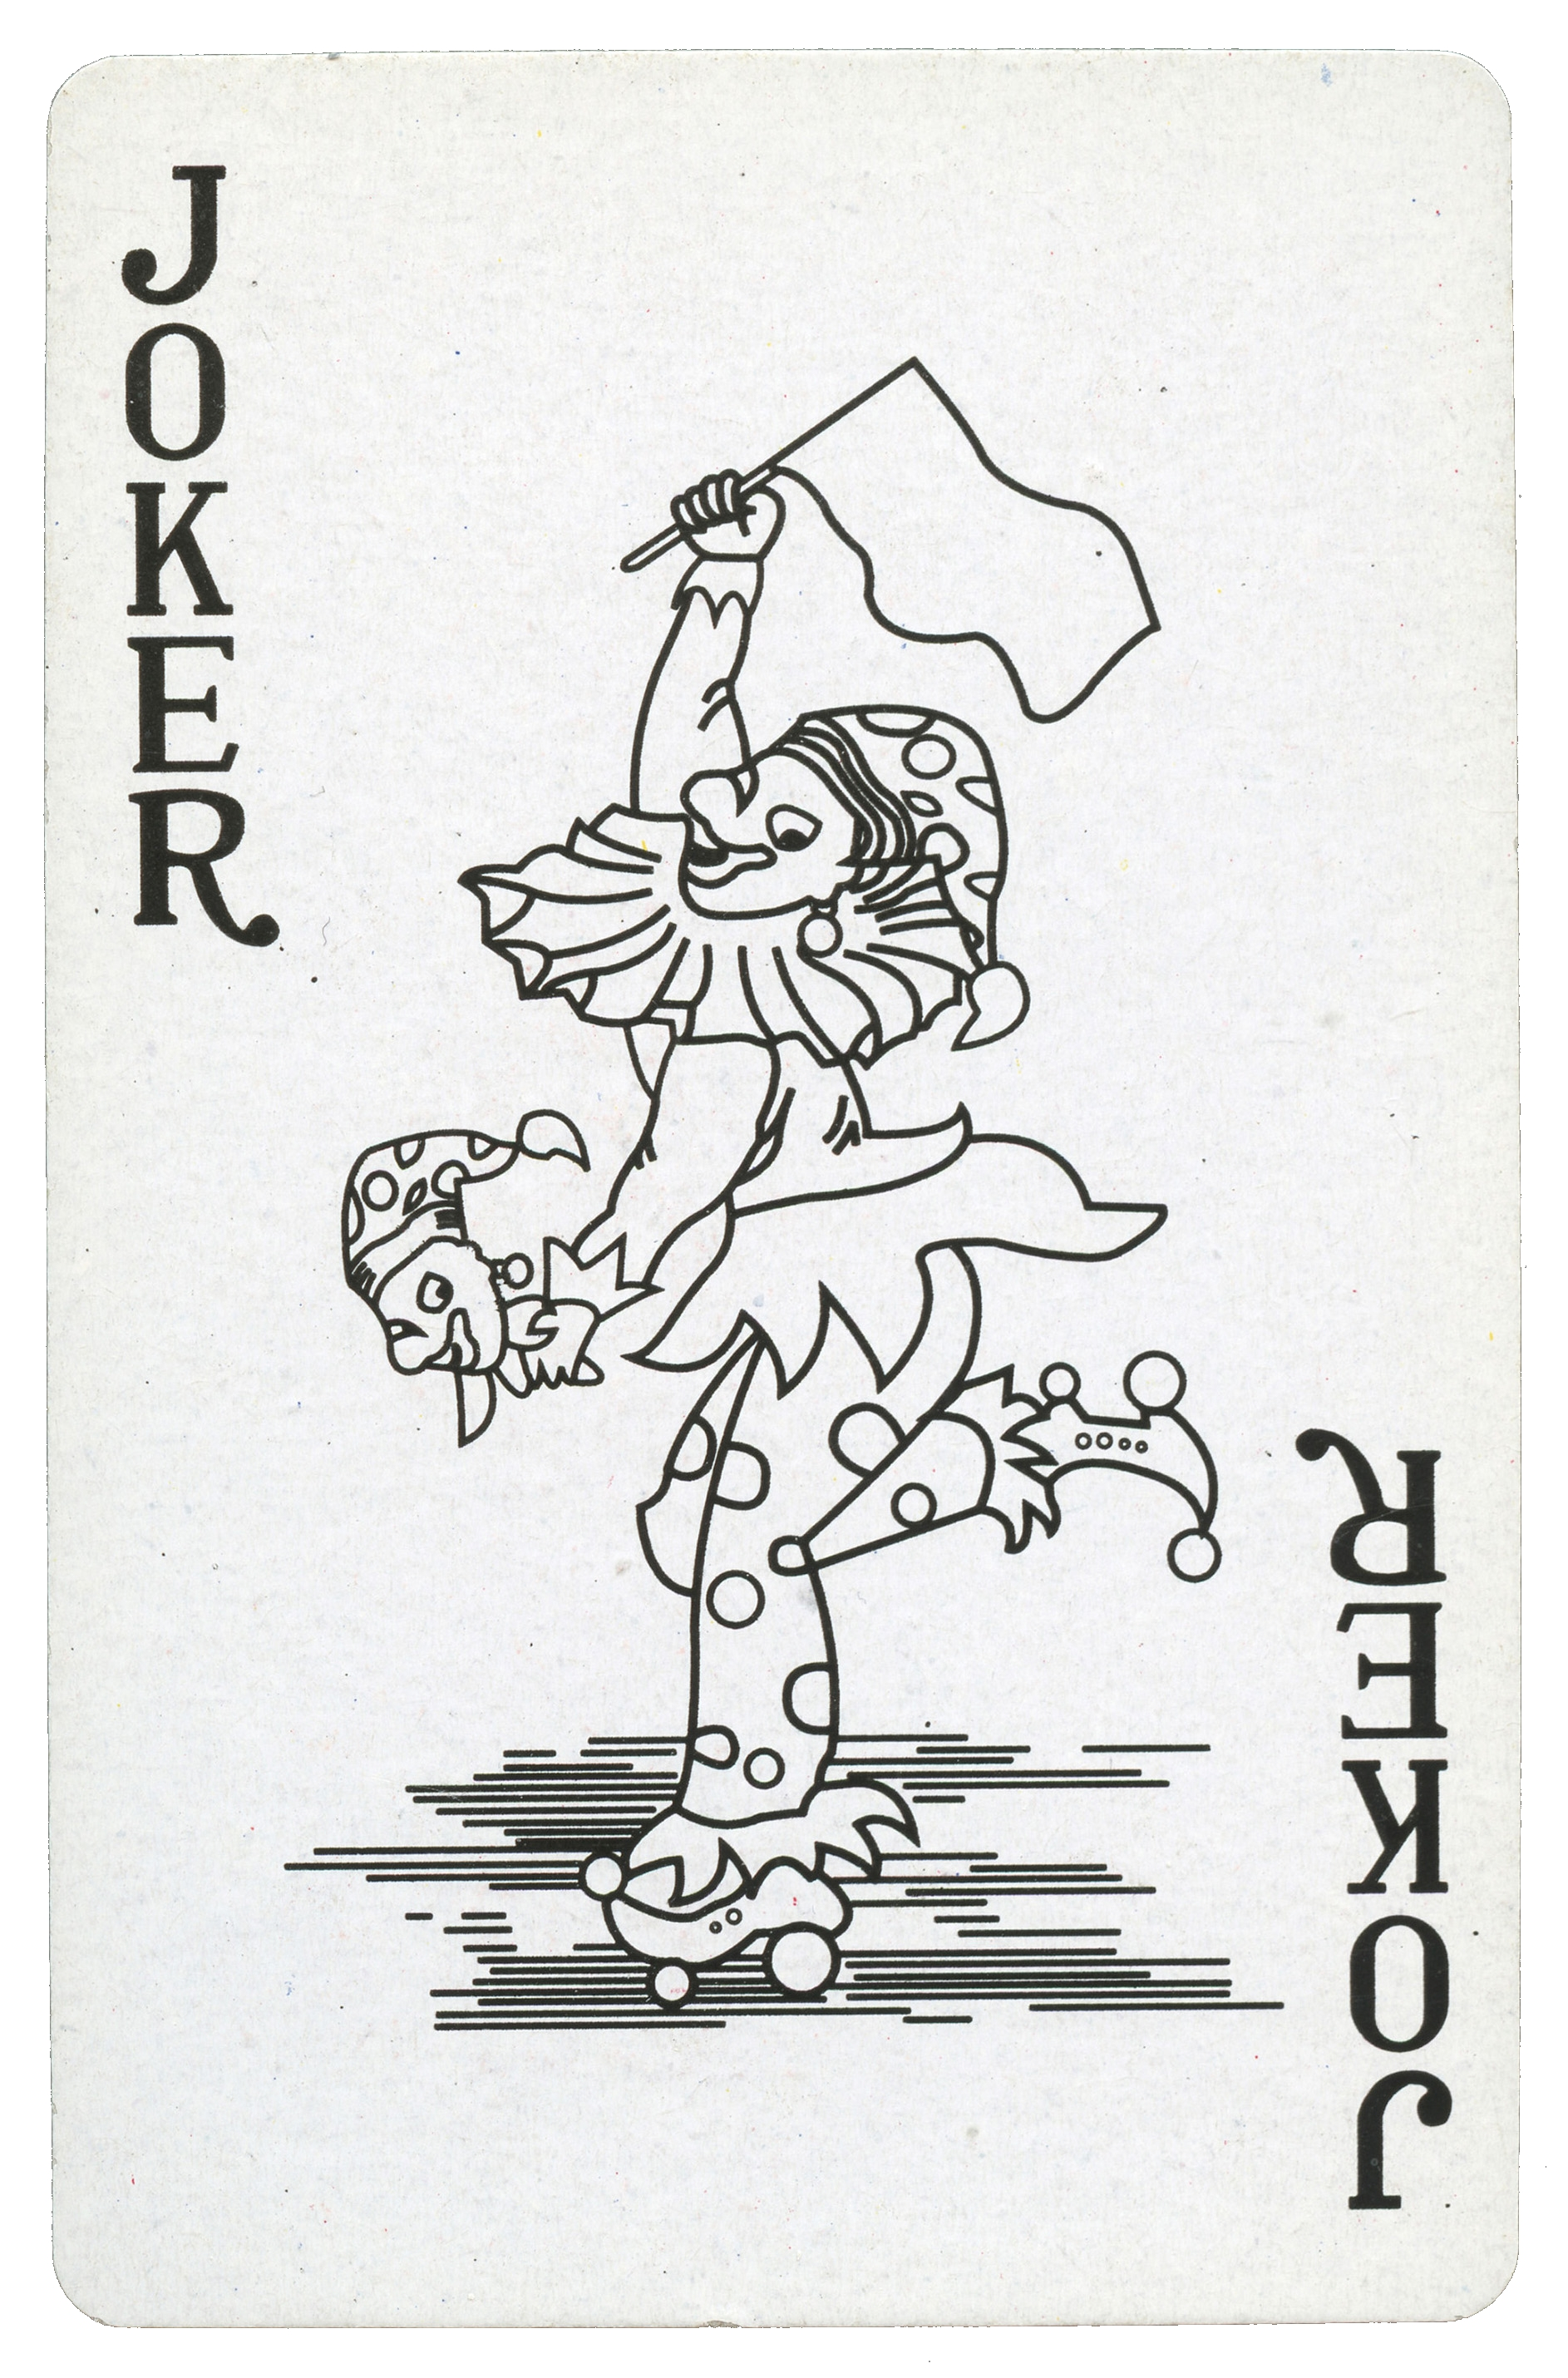
\includegraphics{images/joker-48067975746_0db0b8eba0_o.jpg}
\caption{joker-48067975746}
\end{figure}

\newpage

\hypertarget{matching-a-numeric-sequence}{%
\section{Matching a Numeric
Sequence}\label{matching-a-numeric-sequence}}

Here's a giveaway for you. This puzzle is \emph{possible} to solve. I
won't give you that same assurance when I describe the next two
(related) puzzles.

Regular expressions do not really understand numbers. A `7' or a `777'
might be sequences of digits matched in a string, but they are not
fundamentally different, to regexen, than any other character patterns.
Quantifiers can express numbers, either 0/1 with \texttt{?}, 0 or more
with \texttt{*}, or 1 or more with \texttt{+}. In extended regexen like
Python uses, we can even express specific counts like \texttt{\{3,6\}}
for ``at least three and not more than 6.'' But those are specific
numbers, not calculated quantities.

Nonetheless, we would like to recognize a distinct integer sequence, and
rule out other integer sequences, using a regular expression. The trick
here is that we can represent an integer as repetitions of the same
character, and the number of such repetitions can (to us, at least)
represent numbers.

Specifically, for this puzzle, you would like to identify strings that
represent successive doublings, and exclude all strings that do not have
that pattern. We use the symbol `@' for one unit simply because it is
available and doesn't have special meaning with regex patterns. Spaces
can separate numbers from each other. So for example:

\begin{Shaded}
\begin{Highlighting}[]
\OperatorTok{\textgreater{}\textgreater{}\textgreater{}}\NormalTok{ s1 }\OperatorTok{=} \StringTok{"@@@ @@@@@@ @@@@@@@@@@@@ "} \CommentTok{\# 3 6 12}
\OperatorTok{\textgreater{}\textgreater{}\textgreater{}}\NormalTok{ s2 }\OperatorTok{=} \StringTok{"@ @@ @@@@ @@@@@@@@ @@@@@@@@@@@@@@@@ "} \CommentTok{\# 1 2 4 8 16}
\OperatorTok{\textgreater{}\textgreater{}\textgreater{}}\NormalTok{ s3 }\OperatorTok{=} \StringTok{"@@ @@@@ @@@@@ @@@@@@@@@@ "} \CommentTok{\# 2 4 5 10}
\OperatorTok{\textgreater{}\textgreater{}\textgreater{}}\NormalTok{ s4 }\OperatorTok{=} \StringTok{"@ @ @@ @@@@ "} \CommentTok{\# 1 1 2 4}
\OperatorTok{\textgreater{}\textgreater{}\textgreater{}} \ControlFlowTok{for}\NormalTok{ s }\KeywordTok{in}\NormalTok{ (s1, s2, s3, s4):}
\NormalTok{...     match }\OperatorTok{=}\NormalTok{ re.search(pat, s)}
\NormalTok{...     }\ControlFlowTok{if}\NormalTok{ match:}
\NormalTok{...         }\BuiltInTok{print}\NormalTok{(}\StringTok{"VALID"}\NormalTok{, match.group())}
\NormalTok{...     }\ControlFlowTok{else}\NormalTok{:}
\NormalTok{...         }\BuiltInTok{print}\NormalTok{(}\StringTok{"INVALID"}\NormalTok{, s)}
\NormalTok{...}
\NormalTok{VALID }\OperatorTok{@@@} \OperatorTok{@@@@@@} \OperatorTok{@@@@@@@@@@@@}
\NormalTok{VALID }\OperatorTok{@} \OperatorTok{@@} \OperatorTok{@@@@} \OperatorTok{@@@@@@@@} \OperatorTok{@@@@@@@@@@@@@@@@}
\NormalTok{INVALID }\OperatorTok{@@} \OperatorTok{@@@@} \OperatorTok{@@@@@} \OperatorTok{@@@@@@@@@@}
\NormalTok{INVALID }\OperatorTok{@} \OperatorTok{@} \OperatorTok{@@} \OperatorTok{@@@@}
\end{Highlighting}
\end{Shaded}

\newpage

The pattern you come up with should match strings of any length that
follow the doubling sequence, and should reject strings of any length
that fail to follow it all the way to their end. The final ``number'' in
a string will always be followed by a space, otherwise it won't have
been terminated and shouldn't match.

Before you turn the page\ldots{}

\textbf{Be sure to rule out the strings that do not express the
sequence.}

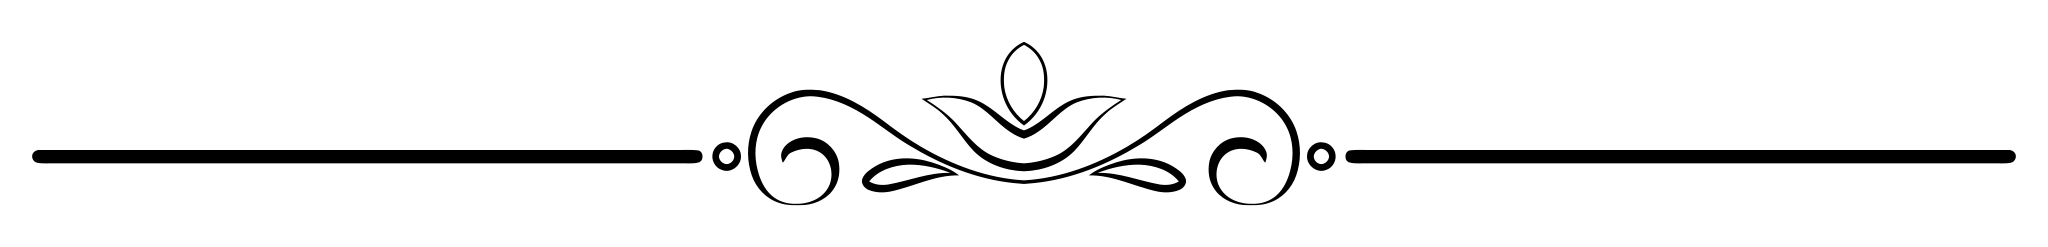
\includegraphics{images/Elegant-Flourish-Frame-Extrapolated-19.svg}

\newpage

Let's start with the solution, then explain why it works.

\begin{Shaded}
\begin{Highlighting}[]
\NormalTok{pat }\OperatorTok{=} \VerbatimStringTok{r"\^{}(((@+) )(?=\textbackslash{}3\textbackslash{}3 ))+(\textbackslash{}3\textbackslash{}3 )$"}
\end{Highlighting}
\end{Shaded}

What we do here is several steps:

First, make sure we are beginning at the start of the string (`\^{}').
This is where `s4' failed; it doubles as a suffix, but we are required
to start at the beginning.

Second, match at least one \texttt{@} symbol, up to however many occur
in a row. After that group of \texttt{@} symbols, we have a space that
is not part of the group.

Third, \emph{lookahead} to a pattern that has twice as many \texttt{@}
symbols as the group we last saw. I spelled that as
\texttt{\textbackslash{}3\textbackslash{}3}, which feels intuitive, but
you could likewise spell it as \texttt{\textbackslash{}3\{2\}} to mean
the same thing.

Fourth, and finally, after all those repetitions of lookaheads and
groups, collect the same pattern as the lookahead just before the end of
the string. We want to have the entire sequence in
\texttt{match.group()}, not to leave off the last ``number.''

\newpage

\hypertarget{matching-the-fibonacci-sequence}{%
\section{Matching the Fibonacci
Sequence}\label{matching-the-fibonacci-sequence}}

Here we get to something harder than the last puzzle. It is not obvious
whether regular expressions are powerful enough to express this
sequence. Think about your solution, or the reasons it is impossible,
before you turn the page.

The Fibonacci sequence is a famous recursive relationship, in which each
number in the sequence is the sum of the prior two numbers. Hence, the
first few Fibonacci numbers are:

\begin{verbatim}
1 1 2 3 5 8 13 21 34 55 89 144
\end{verbatim}

In fact, the Fibonacci sequence is only one of an infinite number of
similar recursive sequences, known generally as Lucas sequences. The
Lucas numbers are one such sequence in which the initial elements are 2
and 1 (rather than 1 and 1). We are actually interested here in matching
``Fibonacci-like'' sequences, where given two elements, the next one is
the sum of those prior two.

As in the last puzzle, we represent numeric sequences by a number of
repetitions of the \texttt{@} symbol followed by spaces. For example:

\begin{Shaded}
\begin{Highlighting}[]
\CommentTok{\# Match: 1 1 2 3 5 8}
\NormalTok{fibs }\OperatorTok{=} \StringTok{"@ @ @@ @@@ @@@@@ @@@@@@@@ "}
\CommentTok{\# Match: 2 1 3 4 7 11}
\NormalTok{lucas }\OperatorTok{=} \StringTok{"@@ @ @@@ @@@@ @@@@@@@ @@@@@@@@@@@ "}
\CommentTok{\# Match: 3 1 4 5 9 14}
\NormalTok{fib2 }\OperatorTok{=} \StringTok{"@@@ @ @@@@ @@@@@ @@@@@@@@@ @@@@@@@@@@@@@@ "}
\CommentTok{\# Fail: 1 1 3 4 7 11}
\NormalTok{wrong1 }\OperatorTok{=} \StringTok{"@ @ @@@ @@@@ @@@@@@@ @@@@@@@@@@@ "}
\CommentTok{\# Fail: 1 1 2 3 4 7}
\NormalTok{wrong2 }\OperatorTok{=} \StringTok{"@ @ @@ @@@ @@@@ @@@@@@@ "}
\end{Highlighting}
\end{Shaded}

Can you create a regular expression that matches only Fibonacci-like
sequences within encoded strings?

Before you turn the page\ldots{}

\textbf{The Golden Spiral beautifully generalizes Fibonacci Numbers.}

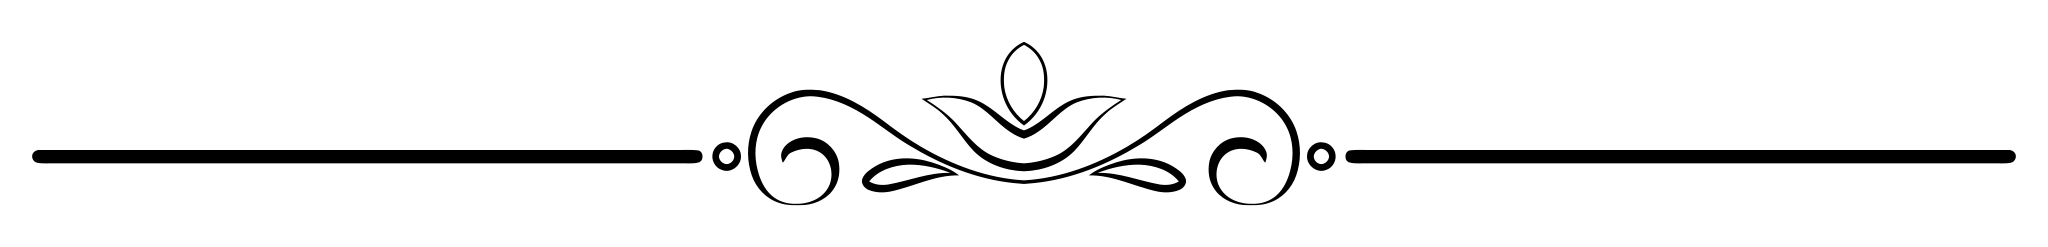
\includegraphics{images/Elegant-Flourish-Frame-Extrapolated-19.svg}

\newpage

It turns out that matching properly encoded Fibonacci-like sequences is
within the power of regular expressions. Adding together two prior
elements is actually a lot like simply doubling the one prior element as
we did in the last puzzle.

The main difference in the solution to this puzzle versus the last one
is that we need to backreference two groups in the lookahead pattern
rather than just one. Study the explanation of the last puzzle before
looking at the solution to this one.

\begin{Shaded}
\begin{Highlighting}[]
\OperatorTok{\textgreater{}\textgreater{}\textgreater{}}\NormalTok{ pat1 }\OperatorTok{=} \VerbatimStringTok{r"\^{}(((@+) (@+) )(?=$|\textbackslash{}3\textbackslash{}4 ))+(\textbackslash{}3\textbackslash{}4)?$"}
\OperatorTok{\textgreater{}\textgreater{}\textgreater{}}\NormalTok{ pat2 }\OperatorTok{=} \VerbatimStringTok{r"\^{}@+ (((@+) (@+) )(?=\textbackslash{}3\textbackslash{}4 ))+"}
\OperatorTok{\textgreater{}\textgreater{}\textgreater{}} \ControlFlowTok{for}\NormalTok{ s }\KeywordTok{in}\NormalTok{ (fibs, lucas, fib2, wrong1, wrong2):}
\NormalTok{...     match }\OperatorTok{=}\NormalTok{ re.search(pat1, s)}
\NormalTok{...     }\ControlFlowTok{if}\NormalTok{ match }\KeywordTok{and}\NormalTok{ re.search(pat2, s):}
\NormalTok{...         }\BuiltInTok{print}\NormalTok{(}\StringTok{"VALID"}\NormalTok{, match.group())}
\NormalTok{...     }\ControlFlowTok{else}\NormalTok{:}
\NormalTok{...         }\BuiltInTok{print}\NormalTok{(}\StringTok{"INVALID"}\NormalTok{, s)}
\NormalTok{...}
\NormalTok{VALID }\OperatorTok{@} \OperatorTok{@} \OperatorTok{@@} \OperatorTok{@@@} \OperatorTok{@@@@@} \OperatorTok{@@@@@@@@}
\NormalTok{VALID }\OperatorTok{@@} \OperatorTok{@} \OperatorTok{@@@} \OperatorTok{@@@@} \OperatorTok{@@@@@@@} \OperatorTok{@@@@@@@@@@@}
\NormalTok{VALID }\OperatorTok{@@@} \OperatorTok{@} \OperatorTok{@@@@} \OperatorTok{@@@@@} \OperatorTok{@@@@@@@@@} \OperatorTok{@@@@@@@@@@@@@@}
\NormalTok{INVALID }\OperatorTok{@} \OperatorTok{@} \OperatorTok{@@@} \OperatorTok{@@@@} \OperatorTok{@@@@@@@} \OperatorTok{@@@@@@@@@@@}
\NormalTok{INVALID }\OperatorTok{@} \OperatorTok{@} \OperatorTok{@@} \OperatorTok{@@@} \OperatorTok{@@@@} \OperatorTok{@@@@@@@}
\end{Highlighting}
\end{Shaded}

Actually, there are two extra caveats here. We assume in this solution
that an even number of numbers are represented in the string. The
lookahead only evaluates the one next number (that must be the sum of
the current two numbers). However, this means that we match two
different `@' sequences at a time; and hence that there must be an even
number if we match to the end.

The second issue is that since we stride two-by-two through the
``numbers,'' we need to use a second regular expression to make sure the
sequence \emph{predicts} the next element when offset by one element as
well. We see that problem in \texttt{wrong1}. If we only utilized
\texttt{pat1} it would incorrectly match as Fibonacci-like. Since
\texttt{pat1} already collects the final ``number,'' there is no need
for \texttt{pat2} to do so as well; the lookahead suffices.

\begin{figure}
\centering

\includegraphics{images/Naive_Scribble_Recto.png}
\caption{Naive\_Scribble\_Recto}
\end{figure}

\newpage

\hypertarget{matching-the-prime-numbers}{%
\section{Matching the Prime Numbers}\label{matching-the-prime-numbers}}

Perhaps surprisingly, in the last puzzle we were able to match
Fibonacci-like sequences using regular expressions. Let's turn next to
whether we might do the same thing with prime numbers. In particular, if
you can find it, your regular expression(s) will only need to match
ascending initial sequences of the primes, but all such initial
sequences.

As in the last two puzzles, we encode numeric sequences using a number
of contiguous \texttt{@} symbols, with each ``number'' separated by
spaces. For example:

\begin{Shaded}
\begin{Highlighting}[]
\CommentTok{\# Match: 2 3 5 7}
\NormalTok{primes4 }\OperatorTok{=} \StringTok{"@@ @@@ @@@@@ @@@@@@@ "}
\CommentTok{\# Match: 2 3 5 7 11}
\NormalTok{primes5 }\OperatorTok{=} \StringTok{"@@ @@@ @@@@@ @@@@@@@ @@@@@@@@@@@ "}
\CommentTok{\# Fail: 2 3 7 11}
\NormalTok{fail1 }\OperatorTok{=} \StringTok{"@@ @@@ @@@@@@@ @@@@@@@@@@@ "}
\CommentTok{\# Fail: 2 3 4 5 7}
\NormalTok{fail2 }\OperatorTok{=} \StringTok{"@@ @@@ @@@@ @@@@@ @@@@@@@ "}
\end{Highlighting}
\end{Shaded}

The Sieve of Eratosthenes is a lovely and ancient algorithm for finding
all the prime numbers. It ``strikes out'' each multiple of a prime as it
steps through all the natural numbers, leaving only primes thereby. In a
compact Python implementation it can look like the below (this can be
made much more efficient, but at the price of more code).

\begin{Shaded}
\begin{Highlighting}[]
\KeywordTok{def}\NormalTok{ get\_primes():}
    \CommentTok{"Simple lazy Sieve of Eratosthenes"}
\NormalTok{    candidate }\OperatorTok{=} \DecValTok{2}
\NormalTok{    found }\OperatorTok{=}\NormalTok{ []}
    \ControlFlowTok{while} \VariableTok{True}\NormalTok{:}
        \ControlFlowTok{if} \BuiltInTok{all}\NormalTok{(candidate }\OperatorTok{\%}\NormalTok{ prime }\OperatorTok{!=} \DecValTok{0} \ControlFlowTok{for}\NormalTok{ prime }\KeywordTok{in}\NormalTok{ found):}
            \ControlFlowTok{yield}\NormalTok{ candidate}
\NormalTok{            found.append(candidate)}
\NormalTok{        candidate }\OperatorTok{+=} \DecValTok{1}
\end{Highlighting}
\end{Shaded}

\newpage

The form of the Sieve is definitely reminiscent of lookahead assertions
which we have used in many of the puzzles. Think about whether you can
implement this using regular expressions (don't think about performance
for this puzzle). Before you look at the discussion, try either to find
a regular expression to match the valid sequences or to formulate
clearly why you cannot.

Before you turn the page\ldots{}

\textbf{Honor the Fundamental Theorem of Arithmetic.}

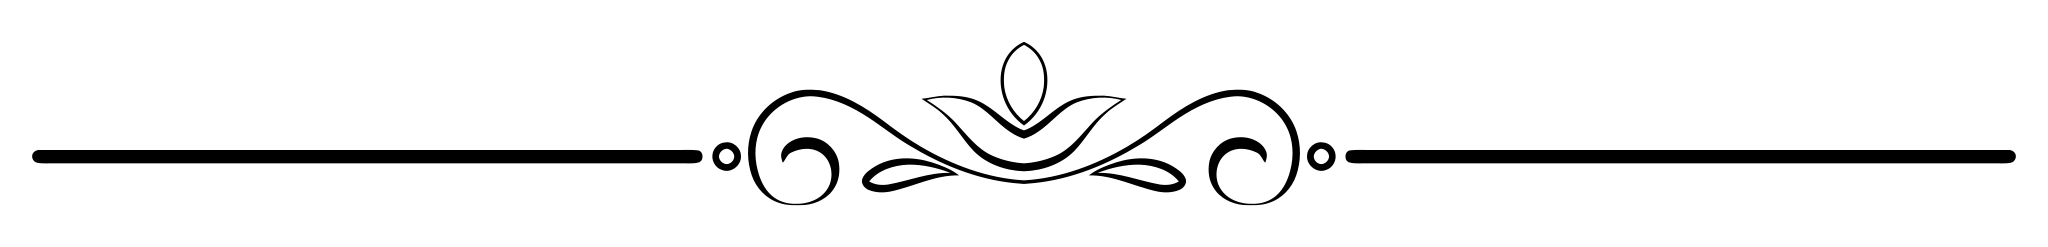
\includegraphics{images/Elegant-Flourish-Frame-Extrapolated-19.svg}

\newpage

This puzzle turns out to be another one that exceeds the ability of
regular expressions. On the face of it, it might seem like
\emph{negative lookahead assertions} are exactly what you would use to
implement the Sieve, or something akin to it. That is, if some group
matched, e.g. \texttt{(@@@)} or \texttt{(@+)}, then you should be able
to backreference to a repetition of that group.

Let's say the hypothetical group was number 7. In that case, a negative
lookahead assertion like \texttt{(?!\ \textbackslash{}7\{2,\}\ )} would
state precisely that no contiguous numbers of \texttt{@} symbols, whose
count is a multiple of the number in the prior match group, occur later
in the string. That sounds a lot like what the Sieve does.

Negative lookahead is indeed a powerful and useful technique. In fact,
you could perfectly well implement a partial sieve to exclude all the
multiples of the first N primes from occurring in a candidate string.
The problem is that regular expressions can only have a finite number of
match groups by definition. That is, regular expressions are a way of
expressing \emph{finite state} machines. The exact maximum number of
groups can vary between regex engines; it is 100 in the Python standard
library \texttt{re} module, 500 in the third-party \texttt{regex}
module, and various other numbers in other programming languages or
libraries. But it is always a finite number.

To match \emph{every} string of initial primes, we need to ``strike
out'' indefinitely many primes along the way. This same problem would
occur for every other sequential prime-finding algorithm. There do exist
direct primality tests that do not iterate through the smaller primes,
such as the probabilistic Miller--Rabin test\footnote{A version of the
  Miller-Rabin test can be made deterministic if the Generalized Riemann
  hypothesis holds.} or the deterministic Agrawal--Kayal--Saxena test.
However, all of those require mathematical calculations that are not
possible in regular expressions.

\begin{figure}
\centering

\includegraphics{images/Olives_Recto.png}
\caption{Olives\_Recto}
\end{figure}

\newpage

\hypertarget{matching-relative-prime-numbers}{%
\section{Matching Relative Prime
Numbers}\label{matching-relative-prime-numbers}}

If you read the last puzzle, you saw the subtle reason why a regular
expression cannot match an initial sequence of primes. Think
\emph{finite} automaton. If you skipped that puzzle, at least go back
and refresh your understanding of the Sieve of Eratosthenes.

Mathematics has a concept of \emph{relative primes} which is slightly
weaker than primality. All prime numbers are relatively prime---also
called \emph{coprime}---with each other, but other pairs are as well.
Two coprime numbers have no common divisors other than 1. This is
certainly true of prime numbers; for example, 11 and 53 are relatively
prime since neither have any divisors other than themselves and 1. But
likewise 10 and 21 are coprime since the divisors of the first are 2 and
5, but those of the second are 3 and 7, which do not overlap.

So the question for this puzzle is whether you can create an expression
that will identify all and only sequences of ascending natural numbers
where all of them are relatively prime to each other. Trivially, any
sequence of ascending primes qualifies here, but so do other sequences.

As in the last three puzzles, we encode numeric sequences using a number
of contiguous \texttt{@} symbols, with each ``number'' separated by
spaces. For example:

\newpage

\begin{Shaded}
\begin{Highlighting}[]
\CommentTok{\# Match: 2 3 5 7 11}
\NormalTok{primes5 }\OperatorTok{=} \StringTok{"@@ @@@ @@@@@ @@@@@@@ @@@@@@@@@@@ "}
\CommentTok{\# Match: 2 5 7 9 11}
\NormalTok{relprime1 }\OperatorTok{=} \StringTok{"@@ @@@@@ @@@@@@@ @@@@@@@@@ @@@@@@@@@@@ "}
\CommentTok{\# Match: 3 4 7 11}
\NormalTok{relprime2 }\OperatorTok{=} \StringTok{"@@@ @@@@ @@@@@@@ @@@@@@@@@@@ "}
\CommentTok{\# Match: 9 16}
\NormalTok{startbig }\OperatorTok{=} \StringTok{"@@@@@@@@@ @@@@@@@@@@@@@@@@ "}
\CommentTok{\# Fail: 2 3 4 5 7  (2, 4 relatively composite)}
\NormalTok{fail1 }\OperatorTok{=} \StringTok{"@@ @@@ @@@@ @@@@@ @@@@@@@ "}
\CommentTok{\# Fail: 5 7 2 3 11 (all primes, non{-}ascending)}
\NormalTok{fail2 }\OperatorTok{=} \StringTok{"@@@@@ @@@@@@@ @@ @@@ @@@@@@@@@@@ "}
\end{Highlighting}
\end{Shaded}

Are relative primes consigned to the same fate as primes?

Before you turn the page\ldots{}

\textbf{Nothing is either true or false but thinking makes it so.}

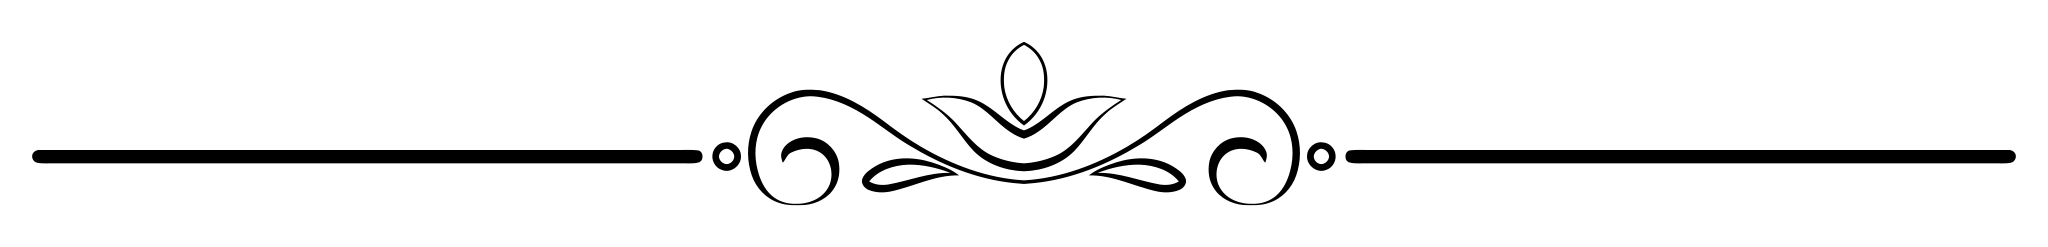
\includegraphics{images/Elegant-Flourish-Frame-Extrapolated-19.svg}

\newpage

There are a couple of issues to consider in this solution. It turns out
that such a solution is indeed possible, using much the same style as
the Sieve of Eratosthenes, but not an identical technique. That is, as
discussed in the last puzzle, we are perfectly well able to reject a
string based on a future multiple of a given number.

The trick is that we do not need to reject \emph{infinitely} many if we
do not assume that a string needs to contain all the initial primes.
Instead, we can focus just on a single number at a time, and rule out
\emph{its} multiples. We might miss some primes in our sequence, or
indeed have some relatively prime composite numbers. But that satisfies
the current puzzle.

However, for this ``striking through'' to work, we need also to enforce
the rule that sequences are ascending. Otherwise, we might encounter,
e.g.~\texttt{@@@@@@@@\ @@@@\ @@} (i.e.~`8 4 2'). Those are definitely
not mutually coprime. However, ``stricking out'' multiples of 8 does not
help reject 4 later in the string. Python only allows fixed length
lookbehind assertions, but some other regex implementation could
technically relax this ascending sequence restriction (however, a
library that did so would quickly face catastrophic exponential
complexity in this case).

\begin{Shaded}
\begin{Highlighting}[]
\NormalTok{pat }\OperatorTok{=} \VerbatimStringTok{r\textquotesingle{}\^{}((@@+) (?=\textbackslash{}2@)(?!.* \textbackslash{}2\{2,\} ))+\textquotesingle{}}
\end{Highlighting}
\end{Shaded}

Here we first identify a group of 2 or more \texttt{@} symbols. Then we
do a postive lookahead to ensure that the next group of \texttt{@}
symbols has at least one more symbol.

The real crux of this is the \emph{negative lookahead} assertion that we
never later see a (space delimited) sequence of two or more copies of
the group. This pattern does not capture the final ``number'' in the
sequence; it is just used to provide a true or false answer to whether
the sequence matches.

\newpage
